\documentclass{article}

% NeurIPS 2025 style. The preprint option shows author names on this draft.
% Drop the option for an anonymized submission.
\usepackage[preprint]{neurips_2025}

\usepackage[utf8]{inputenc}
\usepackage[T1]{fontenc}
\usepackage{hyperref}
\usepackage{url}
\usepackage{booktabs}
\usepackage{amsfonts}
\usepackage{amsmath}
\usepackage{amssymb}
% Aliases so inequality signs stay valid if the source is edited as Markdown.
\newcommand{\lt}{<}\newcommand{\gt}{>}
\usepackage{graphicx}
\usepackage{float}
\usepackage[font=normalsize,labelfont=bf,labelsep=period]{caption}
\captionsetup{font={normalsize},labelfont={bf}}
\usepackage{tikz}
\usetikzlibrary{positioning,arrows.meta,calc}
\usepackage{microtype}
\usepackage{xcolor}
\definecolor{cemepiteal}{HTML}{0E7C7B}
\newcommand{\discutir}[1]{\textcolor{red}{\textbf{[DISCUTIR E ESCREVER: #1]}}}

\title{Forecasting VAT (ICMS) Collection\\
by Type, on the v1 Grains}

\author{%
  \'Etore Braga e Santos \\ Faculdade de Tecnologia - Unicamp \\ CEMEPI-USP \\ PGE-SP \\ \texttt{e285813@dac.unicamp.br}
  \and
  Jo\~ao Bertini \\ FT-Unicamp \\ CEMEPI-USP \\ PGE-SP \\ \texttt{bertini@unicamp.br}
  \and
  Livia Maria Lopes Stanzani \\ FEA-RP/USP \\ CEMEPI-USP \\ \texttt{lmlstanzani@usp.br}
}

\begin{document}

\maketitle

\begin{abstract}
VAT (ICMS) is the value-added tax in this study.
We forecast three collection series from one legal-entity book: the total, Declarado, and Autuado.
The series end on 31 December 2025.
Each series has four grains: month, calendar day, Monday--Friday, and week.
The protocol is the closed v1 benchmark.
The cut is one train block, one validation block, and one test block.
The rank is test sMAPE.
The best model is not the same on every series.
On the monthly grain, boosting leads the total and Autuado, and SARIMAX leads Declarado.
On Monday--Friday, TimesFM leads all three series.
[DISCUTIR E ESCREVER]

\end{abstract}

\section{Introduction}
\label{sec:intro}

VAT (ICMS) is a value-added tax.
This paper forecasts VAT (ICMS) collection, not the mix of all enrolled taxes.
The book has more than one ICMS type.
Declarado is tax the debtor reported.
Autuado is tax from an assessment (\texttt{ICMS Autua\c{c}\~ao}).
Together those two types are almost the whole legal-entity book.
Section~\ref{sec:data} reports the shares.

A grain is the time step of a forecast.
The grains are the v1 grains: month, calendar day (grain A), Monday--Friday (grain B), and week.
Grain B keeps national holidays.
It is not grain A with weekends removed after the score.

The protocol is the closed v1 benchmark.
One series has one contiguous train block, one validation block, and one test block.
The study does not use a rolling origin.
It does not reconcile grains.
It does not add a model family.
The candidates are M0--M9 and E1--E4, as in v1.
The official rank is test sMAPE.
The skill score compares a model with the seasonal naive of the same grain.
A Diebold-Mariano test with the small-sample correction compares the best model with that naive~\citep{diebold1995comparing,harvey1997testing}.
A model confidence set lists the models the test block does not separate~\citep{hansen2011mcs}.

The questions are:
\begin{enumerate}
  \item Which model has the lowest test sMAPE on each series and each grain?
  \item Does that model change between the total, Declarado, and Autuado?
  \item Does the test separate that model from the seasonal naive, and from the other candidates?
\end{enumerate}

[DISCUTIR E ESCREVER]

\section{Related work}
\label{sec:related}

\paragraph{Seasonal baselines and sMAPE.}
Hyndman and Athanasopoulos describe the practice we follow.
Use a seasonal naive baseline.
Select low-order SARIMA models by an information criterion on the training sample.
Do not tune on the test block~\citep{hyndman2021fpp3,box1970tsa}.
The M4 competition ranked many series with sMAPE~\citep{makridakis2020m4}.
No one family won every frequency in that competition.
We use test sMAPE as the rank for a local reason as well.
Plain MAPE divides by the outcome.
That ratio is undefined when collection is zero~\citep{hyndman2006measures}.
sMAPE remains defined as long as the outcome and the forecast are not both zero.

\paragraph{Skill scores.}
Murphy defined a skill score $1 - A/A_{\mathrm{ref}}$ for squared error~\citep{murphy1988skill}.
We use the same ratio with sMAPE in place of squared error.
Murphy did not define an sMAPE skill score.
MASE is the closer forecasting precedent.
MASE divides absolute error by the in-sample absolute error of a seasonal naive forecast~\citep{hyndman2006measures}.
Our skill score is computed on the test block.
It does not replace the sMAPE rank.

\paragraph{Tax forecasting.}
RAMuST is a transformer for industry-level corporate income tax~\citep{you2025ramust}.
It was presented at the NeurIPS 2025 Workshop on Generative AI in Finance.
It mixes monthly macro series with a yearly regime variable.
Our target is collection on debt that is already enrolled.
We observe a stock series and GARE totals.
We do not observe a macro or industry panel.
We therefore compare existing forecasters.
We do not propose a mixed-frequency architecture.

\paragraph{Deep forecasters we cite, and those we fit.}
TimesNet maps a series to a two-dimensional grid of within-period and across-period variation, then applies a vision backbone~\citep{wu2023timesnet}.
We use TimesNet as the backbone of E1.
PatchTST cuts each series into patches and runs a shared transformer on those patches~\citep{nie2023patchtst}.
PatchTST is context for that design.
We do not fit PatchTST.
TimesFM is a pretrained decoder-only forecaster~\citep{das2024timesfm}.
Zero-shot means we do not update its weights on our series.
The weights we load are the later TimesFM 3.0 release~\citep{das2024timesfm}.
TimeGrad forecasts by a conditional denoising diffusion process~\citep{rasul2021timegrad}.
Score-based models estimate the gradient of the log-density and sample with Langevin steps~\citep{song2019score}.
Our E3 and E4 models are small univariate versions of those two ideas.
They are trained on the collection series.
They are not the original multivariate code.

\paragraph{Two different meanings of ``selective.''}
SelectiveNet adds a reject option to a classifier so that some cases are not predicted~\citep{geifman2019selectivenet}.
TEM brings a reject option to forecasting.
An encoder--decoder point forecast is paired with an energy, and high-energy forecasts can be rejected~\citep{brusokas2025tem}.
Selective learning for deep forecasting is a training rule, not a reject option~\citep{fu2025selective}.
It drops uncertain or anomalous time steps from the training loss.
It still emits a forecast at every test time.
E1 is the TEM reject option at test time.
E2 is not TEM.
E2 only compares a boosting forecast with the seasonal naive.

\paragraph{Tests of a forecast rank.}
Diebold and Mariano test equal predictive accuracy from a loss differential~\citep{diebold1995comparing}.
Harvey, Leybourne and Newbold correct that statistic for a short sample~\citep{harvey1997testing}.
Hansen, Lunde and Nason build a set of models that survive a sequence of equivalence tests~\citep{hansen2011mcs}.
This paper uses those three references for the tests in Section~\ref{sec:tests}.
The tests do not choose the rank.
The rank remains test sMAPE.

[DISCUTIR E ESCREVER]

\section{Data}
\label{sec:data}

All series stop on 31 December 2025.
A later payment or a later stock snapshot is not in the sample.
The weekly grain keeps a week only when its Sunday label is on or before that date.
The last weekly label is 28 December 2025.
The three days after that Sunday stay in the daily series.
They do not form a week with a later label.

The target is the sum of \texttt{VALOR\_TOTAL\_GARE}.
That field is the cash amount on the state payment slip.
v1 uses the same field and does not apply a price index.
This paper does not apply one either.
Principal, interest, and fine sum to about 83 percent of the slip total in this extract.
The extract does not store the remaining component.
The ratio is similar for each ICMS type.
The gap is a missing component, not a deflator.
A second price adjustment is not used.

The monthly covariate is the enrolled balance \texttt{VALOR\_SEM\_HONORARIOS} in the snapshot of that month.
That balance is not restated to a base-year price.

The universe is legal-entity ICMS.
In the December snapshot, debts with no CNPJ are 0.48 percent of ICMS stock value.
The forecast series do not add those debts.

\paragraph{Shares.}
Table~\ref{tab:shares} uses the December snapshot for stock and the full sample for collection.
Autuado is \texttt{ICMS Autua\c{c}\~ao}.
Declarado is \texttt{ICMS Declarado}.
The other three ICMS types are each below 0.04 percent of stock and of collection.
Declarado plus Autuado is 99.95 percent of legal-entity ICMS stock and 99.87 percent of collection.
Autuado is most of the stock (72.74 percent).
Declarado is most of the collection (64.63 percent).

\begin{table}[t]
  \caption{Share of legal-entity ICMS value.
  Stock is the December snapshot.
  Collection is \texttt{VALOR\_TOTAL\_GARE} from 4 January 2016 through 31 December 2025.}
  \label{tab:shares}
  \centering
  \small
  \begin{tabular}{lrr}
    \toprule
    Type & Stock (\%) & Collection (\%) \\
    \midrule
    ICMS Autua\c{c}\~ao & 72.74 & 35.24 \\
    ICMS Declarado & 27.21 & 64.63 \\
    ICMS Autua\c{c}\~ao Simples Nacional & 0.03 & 0.09 \\
    ICMS Fecoep & 0.01 & 0.04 \\
    ICMS Altera\c{c}\~ao de GIA & 0.00 & 0.00 \\
    \bottomrule
  \end{tabular}
\end{table}

Figure~\ref{fig:shares} draws the same split with the three small types grouped as Other ICMS.
Autuado is most of the stock.
Declarado is most of the cash that arrives.
A forecast of the total mixes those two shapes.

\begin{figure}[ht]
  \centering
  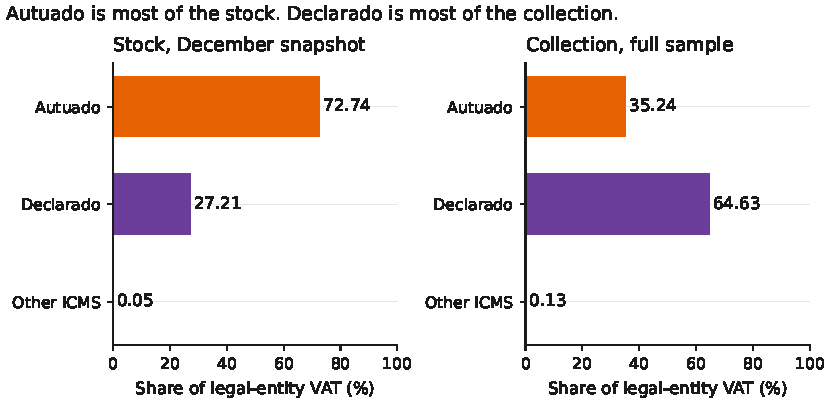
\includegraphics[width=\linewidth]{figures/fig_shares.pdf}
  \caption{Autuado is 72.74 percent of the December stock and 35.24 percent of collection.
  Declarado is 27.21 percent of the stock and 64.63 percent of collection.
  Other ICMS is the three remaining types.
  The two large types are not the same forecasting problem.}
  \label{fig:shares}
\end{figure}

\paragraph{Grains.}
The monthly panel has 120 months, from January 2016 through December 2025.
Tabular models use lags 1, 3, and 12 of collection and the same lags of stock.
The test block is the 12 months of the last year in the sample.
Grain A places the daily slip sum on a calendar and fills missing days with zeros.
The test block is the last 90 days, 3 October through 31 December.
Grain B keeps Monday--Friday and keeps holidays.
The test block is 90 business days, 28 August through 31 December.
The weekly series sums grain A by week ending Sunday.
The test block is 13 weeks, 5 October through 28 December.
The seasonal naive lags are 12, 7, 5, and 52, as in v1.

\section{Method}
\label{sec:method}

\subsection{Steps}
\label{sec:protocol}

The same steps apply to every grain.

\begin{enumerate}
  \item Build the target and the covariates in Section~\ref{sec:data}.
  \item Cut the series into three contiguous blocks: train, validation, and test (Table~\ref{tab:protocol}).
        The cut is a single final window.
        It is not a rolling origin.
  \item Fit each candidate on the train block.
        Choose hyperparameters and thresholds by sMAPE on the validation block.
  \item When the model can be refit, refit the chosen setting on train and validation together.
  \item Forecast the test block.
        Rank models by test sMAPE.
        Do not change any setting after seeing the test block.
\end{enumerate}

Figure~\ref{fig:protocol} draws this path for every grain.
Stage~1 fits the point-forecast families first.
Stage~2 runs after that: E2 needs the Stage~1 boosting and seasonal-naive forecasts, and E1 may use Stage~1 forecasts as energy candidates.
Both stages share the same cut, the same selection step, and the same test rank.
E1 and E2 add an accept-or-abstain rule at forecast time.
The threshold $\tau$ in those rules is chosen in step~3.

\begin{figure}[H]
  \centering
  \resizebox{\linewidth}{!}{%
  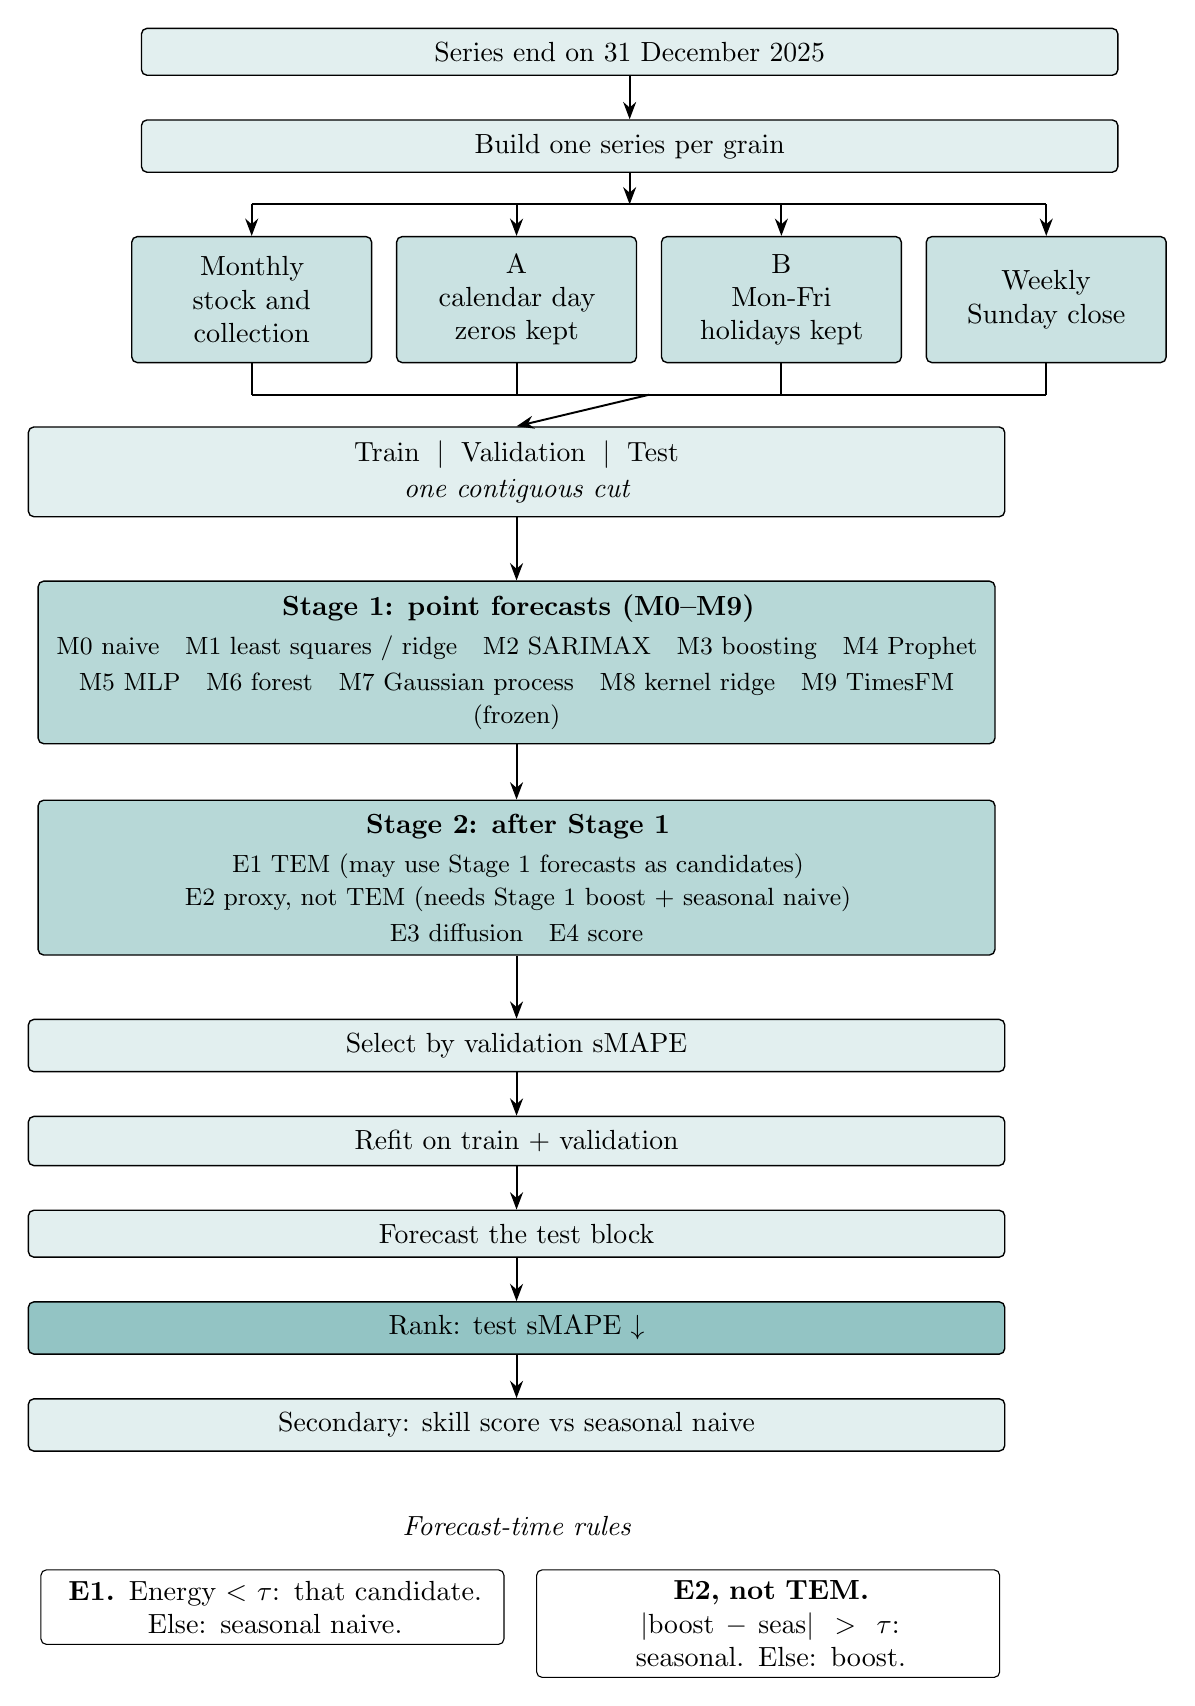
\begin{tikzpicture}[
      font=\normalsize,
      node distance=5.5mm and 3mm,
      wide/.style={draw, rounded corners=2pt, align=center,
                   inner sep=5pt, minimum width=124mm, fill=cemepiteal!12,
                   line width=0.5pt},
      grain/.style={draw, rounded corners=2pt, align=center,
                    inner sep=3.5pt, text width=28mm, minimum height=16mm,
                    fill=cemepiteal!22, line width=0.5pt},
      stage/.style={draw, rounded corners=2pt, align=center,
                    inner sep=5pt, fill=cemepiteal!30, line width=0.5pt},
      rule/.style={draw, rounded corners=2pt, align=center,
                   inner sep=4pt, text width=56mm, fill=white,
                   line width=0.4pt, font=\normalsize},
      arr/.style={-{Stealth[length=2.2mm]}, line width=0.7pt},
      bus/.style={line width=0.7pt}
    ]
    \node[wide] (ex) {Series end on 31 December 2025};
    \node[wide, below=of ex] (build) {Build one series per grain};

    \node[grain, below=8mm of build, anchor=north, xshift=-48mm] (gm)
      {Monthly\\stock and collection};
    \node[grain, right=of gm] (ga) {A\\calendar day\\zeros kept};
    \node[grain, right=of ga] (gb) {B\\Mon-Fri\\holidays kept};
    \node[grain, right=of gb] (gw) {Weekly\\Sunday close};

    \node[wide, below=8mm of ga] (split)
      {Train $\;\vert\;$ Validation $\;\vert\;$ Test\\[1pt]
       {\itshape one contiguous cut}};

    \node[stage, below=8mm of split] (s1)
      {\parbox{118mm}{\centering
        \textbf{Stage 1: point forecasts (M0--M9)}\\[3pt]
        {\small
        M0 naive\quad
        M1 least squares / ridge\quad
        M2 SARIMAX\quad
        M3 boosting\quad
        M4 Prophet\\[1pt]
        M5 MLP\quad
        M6 forest\quad
        M7 Gaussian process\quad
        M8 kernel ridge\quad
        M9 TimesFM (frozen)}
        \par}};

    \node[stage, below=7mm of s1] (s2)
      {\parbox{118mm}{\centering
        \textbf{Stage 2: after Stage 1}\\[3pt]
        {\small
        E1 TEM (may use Stage~1 forecasts as candidates)\\[1pt]
        E2 proxy, not TEM (needs Stage~1 boost $+$ seasonal naive)\\[1pt]
        E3 diffusion\quad
        E4 score}
        \par}};

    \node[wide, below=8mm of s2] (sel) {Select by validation sMAPE};
    \node[wide, below=of sel] (refit) {Refit on train $+$ validation};
    \node[wide, below=of refit] (fc) {Forecast the test block};
    \node[wide, fill=cemepiteal!45, below=of fc] (rank) {Rank: test sMAPE $\downarrow$};
    \node[wide, below=of rank] (skill)
      {Secondary: skill score vs seasonal naive};

    \node[font=\normalsize\itshape, below=7mm of skill] (rtitle)
      {Forecast-time rules};
    \node[rule, below=3mm of rtitle, anchor=north, xshift=-31mm] (c1)
      {\textbf{E1.} Energy $\lt \tau$: that candidate.\\
       Else: seasonal naive.};
    \node[rule, anchor=north west, at={($(c1.north east)+(4mm,0)$)}] (c2)
      {\textbf{E2, not TEM.}\\
       $|\mathrm{boost}-\mathrm{seas}| \gt \tau$: seasonal. Else: boost.};

    \draw[arr] (ex) -- (build);
    \draw[arr] (build.south) -- ++(0,-4mm) coordinate (forkG);
    \draw[bus] (gm.north |- forkG) -- (gw.north |- forkG);
    \foreach \n in {gm,ga,gb,gw}
      \draw[arr] (\n.north |- forkG) -- (\n.north);

    \coordinate (forkS) at ($($(gm.south)!0.5!(gw.south)$)+(0,-4mm)$);
    \draw[bus] (gm.south |- forkS) -- (gw.south |- forkS);
    \foreach \n in {gm,ga,gb,gw}
      \draw[bus] (\n.south) -- (\n.south |- forkS);
    \draw[arr] (forkS) -- (split.north);

    \draw[arr] (split) -- (s1);
    \draw[arr] (s1) -- (s2);
    \draw[arr] (s2) -- (sel);

    \draw[arr] (sel) -- (refit);
    \draw[arr] (refit) -- (fc);
    \draw[arr] (fc) -- (rank);
    \draw[arr] (rank) -- (skill);
  \end{tikzpicture}}
  \caption{Every grain follows one contiguous train, validation, and test cut.
  Stage~1 fits the point-forecast families first.
  Stage~2 runs next.
  E2 needs the Stage~1 boosting forecast and the seasonal naive.
  E1 may use Stage~1 forecasts as energy candidates.
  Settings are chosen by validation sMAPE.
  The chosen model is refit on train plus validation.
  The official rank is test sMAPE.
  The skill score against that grain's seasonal naive is secondary.
  The notes are forecast-time rules only.
  E1 returns the lowest-energy candidate when that energy is below $\tau$, and otherwise the seasonal naive.
  E2 returns the seasonal naive when boosting and the seasonal naive disagree by more than $\tau$, and returns boosting otherwise.
  E2 is not TEM.}
  \label{fig:protocol}
\end{figure}

Some models forecast one step at a time.
At time $t$ they may use only information from before $t$.
Those models are ordinary least squares, ridge, gradient boosting, the forest, the Gaussian process, kernel ridge, and the multilayer perceptron.
The other models forecast the whole test horizon after the refit in step 4.
We do not average ranks across grains.
A kernel-ridge fit with test sMAPE of at least 180 is dropped from the rank.

\begin{table}[t]
  \caption{Blocks and the seasonal naive lag, by grain.
  The seasonal naive lag is the reference in the skill score.
  Validation and test lengths are in periods of that grain.}
  \label{tab:protocol}
  \centering
  \small
  \begin{tabular}{llll}
    \toprule
    Grain & Blocks & Official rank & Seasonal naive \\
    \midrule
    Monthly & train $|$ val 12 $|$ test 12 & test sMAPE & lag 12 \\
    A, calendar day & train $|$ val 90 $|$ test 90 & test sMAPE & lag 7 \\
    B, business day & train $|$ val 90 $|$ test 90 & test sMAPE & lag 5 \\
    Weekly & train $|$ val 13 $|$ test 13 & test sMAPE & lag 52 \\
    \bottomrule
  \end{tabular}
\end{table}

\subsection{sMAPE and the other scores}
\label{sec:metrics}

Let $y_t$ be the observed collection and $\hat y_t$ the forecast.
Let $\epsilon$ be a small positive tolerance.
MAPE averages the absolute percentage error on times with $|y_t| \gt \epsilon$.
A zero collection makes that percentage undefined, so those times are omitted.
sMAPE averages the symmetric percentage error on times with $|y_t| + |\hat y_t| \gt \epsilon$.
The only times sMAPE drops are those where both the outcome and the forecast are zero.
RMSE uses every time in the block.
Write $n_{\mathrm{M}}$ and $n_{\mathrm{S}}$ for the number of times kept by MAPE and by sMAPE.
\begin{align}
  \mathrm{MAPE}
  &= \frac{100}{n_{\mathrm{M}}}
     \sum_{t : |y_t| \gt \epsilon}
     \left|\frac{y_t - \hat y_t}{y_t}\right|,
  \label{eq:mape}\\
  \mathrm{sMAPE}
  &= \frac{100}{n_{\mathrm{S}}}
     \sum_{t : |y_t| + |\hat y_t| \gt \epsilon}
     \frac{2\,|y_t - \hat y_t|}{|y_t| + |\hat y_t|},
  \label{eq:smape}\\
  \mathrm{RMSE}
  &= \sqrt{\frac{1}{n}\sum_{t=1}^{n}(y_t - \hat y_t)^2}.
  \label{eq:rmse}
\end{align}
RMSE is reported as a second description of scale.
It does not decide the rank.
Mean absolute error is computed and is not used to rank models in this extract.
On the monthly panel, exact zeros are rare.
On grain A, zeros are most of the hard days, so sMAPE is the score that still includes them.

\subsection{Skill score}
\label{sec:ss}

Let $A$ be the test sMAPE of a model.
Let $A_{\mathrm{ref}}$ be the test sMAPE of the seasonal naive for that grain (Table~\ref{tab:protocol}).
The skill score is
\begin{equation}
  \mathrm{SS}_{\mathrm{sMAPE}}
  = 1 - \frac{A}{A_{\mathrm{ref}}}.
  \label{eq:ss}
\end{equation}
A positive value means the model has lower test sMAPE than the seasonal naive.
The seasonal naive itself scores zero.
A negative value means higher test sMAPE than the seasonal naive.
The score is undefined when $A_{\mathrm{ref}}$ is near zero or is not a finite number.
On grain B the reference is lag 5.
Lag 1 already beats lag 5 on that series.
Many positive skill scores on B are therefore expected.
They do not mean the formula is wrong.
They also do not mean the model beat a lag-1 forecast.

\subsection{Stage 1 models}
\label{sec:m0m9}

Table~\ref{tab:ladder} names the fourteen forecasts.
The paragraphs below state what each one predicts, which inputs it uses, and how its settings are chosen.

\begin{table}[t]
  \caption{Models in the comparison.
  When a model has settings, validation sMAPE chooses them.}
  \label{tab:ladder}
  \centering
  \small
  \begin{tabular}{llp{6.6cm}}
    \toprule
    ID & Model & What is chosen on validation \\
    \midrule
    M0 & Naive and seasonal naive & Nothing. The seasonal copy is the skill reference. \\
    M1 & Least squares and ridge & Ridge penalty. \\
    M2 & SARIMAX & Order, by AIC on the train block. \\
    M3 & Histogram gradient boosting & Trees, learning rate, and depth. \\
    M4 & Prophet & Trend and seasonality priors. \\
    M5 & Multilayer perceptron & Lag, width, and learning rate. \\
    M6 & Adaptive random forest & Number of trees and feature subsample. \\
    M7 & Gaussian process & Kernel and noise level. \\
    M8 & Kernel ridge & Kernel, penalty, and width. \\
    M9 & TimesFM 3.0 & Nothing. Weights are not updated. \\
    E1 & Selective TEM & Energy threshold. Abstain to the seasonal naive. \\
    E2 & Disagreement proxy & Quantile threshold. Not TEM. \\
    E3 & Residual diffusion & Fixed small sampler. Not the original TimeGrad code. \\
    E4 & Score sampler & Fixed small sampler. \\
    \bottomrule
  \end{tabular}
\end{table}

\paragraph{M0: copy a past value.}
M0 predicts by copying one past observation~\citep{hyndman2021fpp3},
\begin{equation}
  \hat y_t = y_{t-k}.
  \label{eq:m0}
\end{equation}
No coefficient is estimated.
We report $k = 1$ and the seasonal lag in Table~\ref{tab:protocol}: $k \in \{1,12\}$ monthly, $\{1,7,365\}$ on grain A, $\{1,5\}$ on grain B, and $\{1,52\}$ weekly.
The seasonal copy is $A_{\mathrm{ref}}$ in~\eqref{eq:ss}.

\paragraph{M1: least squares and ridge.}
Let $x_t$ be the tabular lags in Section~\ref{sec:data}.
The point forecast is
\begin{equation}
  \hat y_t = x_t^{\top}\beta.
  \label{eq:m1}
\end{equation}
Least squares sets $\alpha = 0$ in the ridge objective~\citep{hoerl1970ridge}
\begin{equation}
  \hat\beta_{\alpha}
  = \arg\min_{\beta}
    \|y - X\beta\|_2^2 + \alpha\|\beta\|_2^2,
  \qquad
  \alpha \in \{0.1, 1, 10\}.
  \label{eq:ridge}
\end{equation}
Validation sMAPE chooses $\alpha$.
Both models then forecast the test block one step at a time.

\paragraph{M2: SARIMAX.}
M2 is a seasonal ARIMA on the target alone.
No extra regressor is passed in~\citep{box1970tsa,hyndman2021fpp3}.
With lag operator $L$ and seasonal period $s$,
\begin{equation}
  \phi_p(L)\,\Phi_P(L^{s})\,(1-L)^{d}\,(1-L^{s})^{D}\, y_t
  = \theta_q(L)\,\Theta_Q(L^{s})\,\varepsilon_t.
  \label{eq:sarimax}
\end{equation}
The period is $s = 12$ monthly, $s = 7$ on grain A, $s = 5$ on grain B, and $s = 4$ weekly.
The weekly skill reference remains lag 52, not this period of 4.
A short grid of orders $(p,d,q)\times(P,D,Q)_s$ is scored by AIC on the train block.
AIC is the Akaike information criterion.
The chosen order is refit on train plus validation and forecasts the whole test horizon.

\paragraph{M3: histogram gradient boosting.}
M3 uses the same $x_t$ as M1.
The prediction is an additive expansion of trees~\citep{friedman2001greedy},
\begin{equation}
  F_M(x) = \sum_{m=1}^{M} \nu\, h_m(x),
  \label{eq:gbm}
\end{equation}
where $h_m$ is a tree fit to the negative gradient of squared error and $\nu$ is the learning rate.
Splits are made on histogram bins.
Each fit may stop early, using 15\% of its current training rows as an internal check.
Validation sMAPE chooses $M$, $\nu$, and the tree depth.
The chosen booster then walks one step at a time through the test block.

\paragraph{M4: Prophet.}
Prophet adds a piecewise linear trend $g(t)$ to a Fourier seasonality $s(t)$~\citep{taylor2018prophet},
\begin{equation}
  y(t) = g(t) + s(t) + \varepsilon_t.
  \label{eq:prophet}
\end{equation}
The published holiday term is omitted.
No holiday calendar is passed in, including on grain B.
Monthly and weekly fits use a yearly cycle.
Daily fits use a weekly cycle and a yearly cycle.
On the monthly panel, validation sMAPE chooses among changepoint prior scales $\{0.05, 0.5\}$ and seasonality prior scales $\{1, 10\}$.
Daily and weekly fits use the single pair $(0.5, 10)$.
The chosen model is refit on train plus validation and forecasts the whole test horizon.

\paragraph{M5: multilayer perceptron.}
M5 maps a window of past target values to the next value~\citep{goodfellow2016dl}.
Let $z_t = (y_{t-L},\ldots,y_{t-1})$ and let $\tilde z_t$ be $z_t$ after a scaler fit on the train block only.
With ReLU $\sigma$ and two hidden layers,
\begin{equation}
  \hat y_t
  = w_3^{\top}\sigma\!\left(W_2\,\sigma(W_1\tilde z_t + b_1) + b_2\right) + b_3.
  \label{eq:mlp}
\end{equation}
Training minimizes squared error and stops if validation squared error stops falling.
We search widths $(32,16)$ and $(64,32)$, step sizes $10^{-3}$ and $3\times 10^{-4}$, and lags $L \in \{6,12\}$ monthly, $\{8,12\}$ weekly, or $\{14,28\}$ daily.
Validation sMAPE, after undoing the scaling, chooses the setting.
We refit on train plus validation and forecast the test block one step at a time with observed lags.
This is a lag-window MLP.
It is not the N-BEATS basis-expansion model.

\paragraph{M6: adaptive random forest.}
M6 predicts the tabular row $x_t$ by an average of regression trees,
\begin{equation}
  \hat y_t = \frac{1}{M}\sum_{m=1}^{M} h_m(x_t).
  \label{eq:arf}
\end{equation}
Trees can be replaced when their error changes~\citep{gomes2017arf}.
The cited paper is about classification.
We use the regression form of that ensemble.
The forest first learns the history before the forecast origin.
It then predicts the next row and updates on the revealed outcome.
Validation sMAPE chooses the number of trees and the feature subsample.

\paragraph{M7: Gaussian process.}
M7 places a Gaussian process prior on a latent function of the tabular covariates~\citep{rasmussen2006gp},
\begin{equation}
  f \sim \mathcal{GP}(0, k),
  \qquad
  y_i = f(x_i) + \varepsilon_i,
  \qquad
  \varepsilon_i \sim \mathcal{N}(0, \alpha).
  \label{eq:gp}
\end{equation}
The forecast we rank is the posterior mean at a new row $x_{\star}$,
\begin{equation}
  \hat y_{\star}
  = k(x_{\star}, X)\,
    \bigl(K(X,X) + \alpha I\bigr)^{-1} y.
  \label{eq:gp-mean}
\end{equation}
On the monthly panel, validation sMAPE chooses among a radial-basis kernel, a Mat\'ern kernel, and a rational-quadratic kernel, each with $\alpha \in \{10^{-2}, 10^{-1}\}$.
Daily fits use a radial-basis kernel and at most 200 training rows, because this inverse grows with the cube of the sample size.
A fit with no finite forecast is omitted.

\paragraph{M8: kernel ridge.}
M8 solves the ridge problem in the feature space of a kernel $k$, on the same columns as M1, after scaling on the train block~\citep{murphy2012ml}.
The dual forecast is
\begin{equation}
  \hat y(x) = \sum_{i=1}^{n} a_i\, k(x, x_i),
  \qquad
  (K + \lambda I)\, a = y.
  \label{eq:krr}
\end{equation}
The kernel is radial basis or Laplacian.
Validation sMAPE chooses that kernel, the penalty $\lambda$, and the kernel width.
A test sMAPE of at least 180 removes that fit from the rank.

\paragraph{M9: TimesFM 3.0.}
TimesFM is a pretrained forecasting model~\citep{das2024timesfm}.
We load TimesFM 3.0 and do not update its weights~\citep{das2024timesfm}.
If $T$ is the last time in the validation block and $H$ is the test length,
\begin{equation}
  (\hat y_{T+1},\ldots,\hat y_{T+H})
  = f_{\theta}(y_1,\ldots,y_T),
  \label{eq:timesfm}
\end{equation}
with $\theta$ held fixed.
We rank the model's mean forecast.
If the weights cannot be loaded, that grain has no M9 row.
We do not substitute another model.

\subsection{Stage 2 models}
\label{sec:energy}

Stage~2 comes after Stage~1.
It asks two further questions.
Does an energy threshold lower test sMAPE relative to the seasonal naive?
Does a simpler switch, with no energy, do so?
E2 reuses Stage~1 boosting and seasonal-naive forecasts.
Only E1 is TEM.

\paragraph{E1: selective TEM.}
E1 assigns an energy $E_{\theta}(x, y)$ to a context $x$ and a candidate value $y$~\citep{brusokas2025tem}.
The implied weight on that candidate is
\begin{equation}
  p_{\theta}(y \mid x) \propto \exp\bigl(-E_{\theta}(x, y)\bigr).
  \label{eq:ebm}
\end{equation}
A lower energy means a higher weight.
The backbone is TimesNet~\citep{wu2023timesnet}, trained with the published TEM code on the splits in Table~\ref{tab:protocol}.
It sees 12 past months, with a 6-month decoder overlap, or 28 past days, with a 14-day overlap, and it predicts one step.
The monthly run uses about 15 forecast epochs and 10 energy epochs.
Daily runs are capped at about 3 epochs of each.
If TimesNet does not finish, we use the published MLP energy model.
That fallback is still TEM.
Candidates are the seasonal naive, the boosting forecast, and the TimesNet forecast when it exists.
$\tau$ is the validation threshold with the lowest validation sMAPE.
With $\mathcal{C}_t$ the candidate set and $k$ the seasonal lag,
\begin{equation}
  \hat y_t =
  \begin{cases}
    \arg\min_{c \in \mathcal{C}_t} E_{\theta}(x_t, \hat y_t^{(c)})
      & \text{if }\min_{c} E_{\theta}(x_t, \hat y_t^{(c)}) \lt \tau, \\[4pt]
    y_{t-k}
      & \text{otherwise.}
  \end{cases}
  \label{eq:tem}
\end{equation}
The second line is abstention.
Coverage is the share of test times that take the first line.
The sMAPE tables do not report coverage.

\paragraph{E2: disagreement proxy.}
E2 predicts either the Stage~1 boosting forecast or the Stage~1 seasonal naive.
It does not compute~\eqref{eq:ebm}.
Those two Stage~1 forecasts must exist before E2 is evaluated.
At each time let
\begin{equation}
  E_t = \bigl|\hat y_t^{\mathrm{boost}} - \hat y_t^{\mathrm{seas}}\bigr|.
  \label{eq:proxy}
\end{equation}
$E_t$ is large when the two forecasts disagree.
On the validation block we set $\tau$ to a quantile of $E_t$.
We try the quantile levels $0.5, 0.6, 0.7, 0.8, 0.9$ and keep the level with the lowest validation sMAPE.
The test rule is
\begin{equation}
  \hat y_t =
  \begin{cases}
    \hat y_t^{\mathrm{seas}} & \text{if } E_t \gt \tau, \\
    \hat y_t^{\mathrm{boost}} & \text{otherwise.}
  \end{cases}
  \label{eq:proxy-rule}
\end{equation}
Disagreement above $\tau$ returns the seasonal naive.
Disagreement at or below $\tau$ returns the boosting forecast.
The name TEM is reserved for E1.

\paragraph{E3: a small diffusion sampler.}
E3 predicts the next scaled value by averaging reverse-diffusion samples~\citep{rasul2021timegrad}.
A three-layer network $\epsilon_{\theta}$ reads a lag window, a noisy target, and a diffusion-time index.
The training corruption at step $k$, and the loss, are
\begin{equation}
  y^{(k)} = \sqrt{\bar\alpha_k}\, y + \sqrt{1 - \bar\alpha_k}\,\epsilon,
  \qquad
  \mathcal{L}
  = \bigl\|\epsilon_{\theta}(x, y^{(k)}, k) - \epsilon\bigr\|_2^2,
  \label{eq:ddpm}
\end{equation}
with $\epsilon \sim \mathcal{N}(0,1)$.
The point forecast is the mean of $S$ reverse trajectories, mapped back to the original scale.
Monthly fits use lag 12, 20 steps, and $S = 8$.
Daily fits use lag 28, 15 steps, $S = 4$, and a subset of the training windows.
Weekly fits use lag 12, 15 steps, and $S = 4$.
This is the denoising step of TimeGrad on one series.
It is not the published multivariate TimeGrad model.

\paragraph{E4: a small score sampler.}
E4 predicts the next scaled value by averaging Langevin chains~\citep{song2019score}.
At noise scale $\sigma = 0.5$, the network $s_{\theta}$ is trained so that, at a point corrupted by $\sigma\epsilon$,
\begin{equation}
  s_{\theta}(x, y + \sigma\epsilon) \approx -\epsilon / \sigma^{2}.
  \label{eq:score-target}
\end{equation}
Sampling repeats
\begin{equation}
  y \leftarrow y + \eta\, s_{\theta}(x, y) + \sqrt{2\eta}\,\xi,
  \qquad
  \xi \sim \mathcal{N}(0,1),
  \label{eq:langevin}
\end{equation}
with step $\eta = 0.05$.
The point forecast is the mean of the chains, after undoing the scaling.
Monthly fits use lag 12, 30 steps, and 6 chains.
Daily and weekly fits use 20 steps and 4 chains, with the same lags as E3.
The network is small and is trained only on this series.

\subsection{Tests after the rank}
\label{sec:tests}

The rank stays test sMAPE.
Two tests describe that rank.
They do not change it.

The Diebold-Mariano test compares the best model with the seasonal naive of the same grain~\citep{diebold1995comparing}.
The loss is the summand inside sMAPE.
The horizon in the Harvey-Leybourne-Newbold correction is one step~\citep{harvey1997testing}.
The corrected statistic is compared with a Student-$t$ distribution on $n-1$ degrees of freedom.
The test is two-sided.
A negative statistic means the best model has lower loss than the seasonal naive.

The model confidence set uses level 0.10~\citep{hansen2011mcs}.
The statistic is the largest $t$ of a model against the average loss of the other models.
A circular block bootstrap with 999 draws gives the p-value.
The block length is the cube root of the test length.
A model leaves the set when the equivalence test rejects.

\subsection{Where the numbers come from}
\label{sec:repro}

This paper states the series, the splits, the scores, and the decision rules.
The model bodies are the v1 notebook
\path{projects/monitoramento/notebooks/articles/arrecadacao_forecast_paper_v1.ipynb}.
The segment run is
\path{projects/monitoramento/notebooks/articles/arrecadacao_forecast_v1_segmentado.ipynb}.
The saved forecasts are under
\path{projects/monitoramento/notebooks/articles/arrecadacao_forecast_v1_segmentado/results/}.
E1 calls the published TEM code.
That vendor tree is not in this worktree, so E1 has no score.
M9 uses the public weights \texttt{google/timesfm-3.0-pytorch}.
Every number in Section~\ref{sec:results} is read from those saved tables.

\section{Results}
\label{sec:results}

Every number below is read from the saved tables for the three VAT series.
The rank is test sMAPE.
Lower is better.
The skill score is higher when the model beats the seasonal naive of that grain.
The HLN column is the two-sided p-value of the leader against that naive.
The model confidence set uses level 0.10.

\subsection{The lowest sMAPE is not the same model}
\label{sec:top3}

Table~\ref{tab:best} names the lowest test sMAPE on each series and grain.
No model leads all twelve cells.
Boosting leads the monthly total and monthly Autuado.
SARIMAX leads monthly Declarado.
Ridge leads the weekly total and weekly Declarado.
Least squares leads weekly Autuado.
TimesFM leads all three Monday to Friday series, and it also leads calendar-day Autuado.
The forest leads calendar-day total and calendar-day Declarado.
E2, the disagreement proxy, does not lead any cell.
E1 has no row.

\begin{table}[ht]
  \caption{Lowest test sMAPE on each series and grain.
  Skill is \(1 - \mathrm{sMAPE}/\mathrm{sMAPE}_{\mathrm{naive}}\) against the seasonal naive of that grain.
  HLN \(p\) is the two-sided Diebold-Mariano test of that leader against the same naive, with the small-sample correction.
  A p-value below 0.05 is discussed in the text.
  It is not a second rank.}
  \label{tab:best}
  \centering
  \scriptsize
  % Generated by make_segment_figures.py. Do not edit the numbers.
\begin{tabular}{lllcrrr}
\toprule
Series & Grain & Best & $n$ & sMAPE & Skill & HLN $p$ \\
\midrule
Total & Month & M3 boosting & 12 & 12.94 & 0.513 & 0.022 \\
Total & Week & M1 ridge & 13 & 41.00 & 0.135 & 0.638 \\
Total & Mon to Fri & M9 TimesFM & 90 & 65.05 & 0.393 & $<0.001$ \\
Total & Calendar day & M6 forest & 90 & 90.52 & 0.149 & 0.717 \\
Declarado & Month & M2 SARIMAX & 12 & 6.79 & 0.602 & 0.040 \\
Declarado & Week & M1 ridge & 13 & 27.48 & 0.180 & 0.246 \\
Declarado & Mon to Fri & M9 TimesFM & 90 & 61.35 & 0.401 & $<0.001$ \\
Declarado & Calendar day & M6 forest & 90 & 78.43 & 0.221 & 0.069 \\
Autuado & Month & M3 boosting & 12 & 20.91 & 0.523 & 0.077 \\
Autuado & Week & M1 least squares & 13 & 52.50 & 0.139 & 0.590 \\
Autuado & Mon to Fri & M9 TimesFM & 90 & 90.32 & 0.255 & $<0.001$ \\
Autuado & Calendar day & M9 TimesFM & 90 & 112.99 & 0.101 & 0.437 \\
\bottomrule
\end{tabular}

\end{table}

Read the skill column before the p-value.
Every leader has positive skill, so every leader beats its seasonal naive on sMAPE.
The size of that win is not the same.
Monthly Declarado has skill 0.602.
The three weekly leaders have skill between 0.135 and 0.180.
A small positive skill means the sMAPE values are close.
The p-value then asks whether the test block can tell them apart.

Table~\ref{tab:top3} lists the next two models.
On several grains the second model is close to the leader.
On the weekly total, ridge is 41.00 and least squares is 41.41.
On Monday to Friday, boosting is within 5 percent of TimesFM on the total and on Declarado.
A chart that draws only the leader would hide that tie.
The forecast figures in Section~\ref{sec:discussion} draw the second model when its test sMAPE is within 5 percent of the leader.
Family-level bars for every model are in Appendix~\ref{app:bars}.

\begin{table}[ht]
  \caption{Three lowest test sMAPE values on each series and grain.
  E2 is the disagreement proxy.
  E2 is not TEM, and E2 is not in this top three except on weekly Declarado, where it is third.}
  \label{tab:top3}
  \centering
  \scriptsize
  % Generated by make_segment_figures.py. Do not edit the numbers.
\begin{tabular}{llllrr}
\toprule
Series & Grain & Rank & Model & sMAPE & Skill \\
\midrule
Total & Month & 1 & M3 boosting & 12.94 & 0.513 \\
 &  & 2 & M0 lag-1 & 15.37 & 0.421 \\
 &  & 3 & M8 kernel ridge & 15.95 & 0.399 \\
\addlinespace
Total & Week & 1 & M1 ridge & 41.00 & 0.135 \\
 &  & 2 & M1 least squares & 41.41 & 0.126 \\
 &  & 3 & M3 boosting & 43.06 & 0.091 \\
\addlinespace
Total & Mon to Fri & 1 & M9 TimesFM & 65.05 & 0.393 \\
 &  & 2 & M3 boosting & 66.02 & 0.384 \\
 &  & 3 & M8 kernel ridge & 71.87 & 0.330 \\
\addlinespace
Total & Calendar day & 1 & M6 forest & 90.52 & 0.149 \\
 &  & 2 & M0 seasonal (365) & 105.47 & 0.009 \\
 &  & 3 & M9 TimesFM & 105.52 & 0.008 \\
\addlinespace
Declarado & Month & 1 & M2 SARIMAX & 6.79 & 0.602 \\
 &  & 2 & E3 TimeGrad & 9.30 & 0.455 \\
 &  & 3 & M4 Prophet & 10.20 & 0.403 \\
\addlinespace
Declarado & Week & 1 & M1 ridge & 27.48 & 0.180 \\
 &  & 2 & M1 least squares & 27.89 & 0.167 \\
 &  & 3 & E2 proxy & 32.07 & 0.043 \\
\addlinespace
Declarado & Mon to Fri & 1 & M9 TimesFM & 61.35 & 0.401 \\
 &  & 2 & M3 boosting & 63.47 & 0.380 \\
 &  & 3 & M8 kernel ridge & 70.88 & 0.308 \\
\addlinespace
Declarado & Calendar day & 1 & M6 forest & 78.43 & 0.221 \\
 &  & 2 & M0 seasonal (7) & 100.73 & 0.000 \\
 &  & 3 & M9 TimesFM & 100.85 & -0.001 \\
\addlinespace
Autuado & Month & 1 & M3 boosting & 20.91 & 0.523 \\
 &  & 2 & M8 kernel ridge & 22.83 & 0.479 \\
 &  & 3 & M2 SARIMAX & 30.72 & 0.298 \\
\addlinespace
Autuado & Week & 1 & M1 least squares & 52.50 & 0.139 \\
 &  & 2 & M8 kernel ridge & 53.80 & 0.118 \\
 &  & 3 & M3 boosting & 54.01 & 0.114 \\
\addlinespace
Autuado & Mon to Fri & 1 & M9 TimesFM & 90.32 & 0.255 \\
 &  & 2 & M8 kernel ridge & 95.16 & 0.215 \\
 &  & 3 & M6 forest & 95.56 & 0.212 \\
\addlinespace
Autuado & Calendar day & 1 & M9 TimesFM & 112.99 & 0.101 \\
 &  & 2 & M6 forest & 114.36 & 0.090 \\
 &  & 3 & M3 boosting & 120.94 & 0.038 \\
\bottomrule
\end{tabular}

\end{table}

\subsection{Monthly panel}
\label{sec:monthly}

On the monthly total, boosting has test sMAPE 12.94 and skill 0.513.
The seasonal naive, lag 12, has sMAPE 26.55.
Lag 1 is second, at 15.37, and kernel ridge is third, at 15.95.
The HLN p-value against the seasonal naive is 0.022.
That rejects equal accuracy with the lag-12 naive at the 5 percent level.
It does not test boosting against lag 1.
The gap from 12.94 to 15.37 is smaller than the gap from 12.94 to 26.55.

On monthly Declarado, SARIMAX has test sMAPE 6.79 and skill 0.602.
The seasonal naive is 17.07.
TimeGrad is second, at 9.30, and Prophet is third, at 10.20.
The HLN p-value is 0.040.
Declarado is the smoothest of the three monthly series, and the absolute error is the smallest.

On monthly Autuado, boosting has test sMAPE 20.91 and skill 0.523.
The seasonal naive is 43.79.
Kernel ridge is second, at 22.83.
The HLN p-value is 0.077.
The point rank favors boosting.
The test does not reject equal accuracy with the seasonal naive at the 5 percent level.

E2 does not lead the month on any series.
On the total its sMAPE is about 21.6, behind boosting, lag 1, and kernel ridge.
On Declarado it is about 16.4, close to the seasonal naive at 17.07 and behind SARIMAX.
A gain for E2 would not be a gain for E1.
E1 is not in the table.

TimesFM does not lead the month.
On the total its sMAPE is about 22.4, which still beats the seasonal naive and loses to boosting.
On Declarado and on Autuado, TimesFM is worse than the seasonal naive.

Table~\ref{tab:monthly} continues each monthly list to eight models.
The order inside Declarado is not the order inside the total.
Prophet and the perceptron sit near the top of Declarado and not at the top of the total.

\begin{table}[t]
  \caption{Monthly grain: eight lowest test sMAPE values on each series.}
  \label{tab:monthly}
  \centering
  \small
  % Generated by make_segment_figures.py. Do not edit the numbers.
\begin{tabular}{llrr}
\toprule
Series & Model & sMAPE & Skill \\
\midrule
Total & M3 boosting & 12.94 & 0.513 \\
 & M0 lag-1 & 15.37 & 0.421 \\
 & M8 kernel ridge & 15.95 & 0.399 \\
 & M4 Prophet & 18.45 & 0.305 \\
 & M1 ridge & 19.07 & 0.282 \\
 & M1 least squares & 19.07 & 0.282 \\
 & E4 ScoreGrad & 19.47 & 0.266 \\
 & M2 SARIMAX & 20.04 & 0.245 \\
\addlinespace
Declarado & M2 SARIMAX & 6.79 & 0.602 \\
 & E3 TimeGrad & 9.30 & 0.455 \\
 & M4 Prophet & 10.20 & 0.403 \\
 & M5 MLP & 10.44 & 0.388 \\
 & M3 boosting & 12.26 & 0.282 \\
 & E4 ScoreGrad & 12.47 & 0.270 \\
 & M8 kernel ridge & 12.49 & 0.268 \\
 & M1 ridge & 12.84 & 0.248 \\
\addlinespace
Autuado & M3 boosting & 20.91 & 0.523 \\
 & M8 kernel ridge & 22.83 & 0.479 \\
 & M2 SARIMAX & 30.72 & 0.298 \\
 & M0 lag-1 & 30.82 & 0.296 \\
 & E2 proxy & 37.71 & 0.139 \\
 & M0 seasonal (12) & 43.79 & 0.000 \\
 & M4 Prophet & 44.38 & -0.014 \\
 & M1 least squares & 44.98 & -0.027 \\
\bottomrule
\end{tabular}

\end{table}

\subsection{Grain A and grain B}
\label{sec:ablation}

Table~\ref{tab:ablation} puts the two daily targets side by side.
Grain A keeps every calendar day, including weekend and empty-slip zeros.
Grain B keeps Monday to Friday and keeps national holidays.

On grain A the sMAPE level is high: 90.52 on the total, 78.43 on Declarado, and 112.99 on Autuado.
The forest leads the total and Declarado.
TimesFM leads Autuado, and the forest is second there (114.36 against 112.99).
On the total, the lag-365 naive (105.47) and TimesFM (105.52) are almost tied, and both are close to the lag-7 naive (106.41).
The HLN p-values on grain A are 0.717 (total), 0.069 (Declarado), and 0.437 (Autuado).
None of them is below 0.05.
Positive skill on grain A is a small gap next to a naive that already copies last week, including the weekend zeros.

On grain B the leader is TimesFM on all three series.
Test sMAPE is 65.05 (total), 61.35 (Declarado), and 90.32 (Autuado).
Skill is 0.393, 0.401, and 0.255 against the lag-5 naive.
The HLN p-value is below 0.001 on every series.
Dropping weekends lowers the sMAPE level on the total and on Declarado, and it changes the leader from the forest to TimesFM.
On Autuado the leader is TimesFM on both daily grains, and the sMAPE level is still the highest of the three series.
The seasonal naive is inside the top three on grain A for the total and for Declarado.
It is outside the top three on grain B.

\begin{table}[ht]
  \caption{Three lowest test sMAPE values on grain A and on grain B.}
  \label{tab:ablation}
  \centering
  \scriptsize
  % Retired. The segment benchmark uses Table tab:best in sections/05_results.tex.

\end{table}

The positive-day score on A is not the official rank.
Scoring only days with a slip answers a different question.
Ranking A is the error on the calendar, zeros included.

\subsection{Weekly series}
\label{sec:weekly}

Ridge leads the weekly total at sMAPE 41.00, and least squares is 41.41.
Ridge leads weekly Declarado at 27.48, and least squares is 27.89.
Least squares leads weekly Autuado at 52.50, with kernel ridge at 53.80 and boosting at 54.01.
The seasonal naive is 47.38, 33.50, and 60.99 on those three series.
Skill is 0.135, 0.180, and 0.139.
The HLN p-values are 0.638, 0.246, and 0.590.
The week has a lowest sMAPE.
The 13-point test does not separate that model from the seasonal naive.
TimesFM is worse than the seasonal naive on all three weekly series.

The test block has 13 weeks.
The gap describes this window.
It is not a standard error for a long-run difference.

\subsection{What each test is saying}
\label{sec:read-tests}

The three tools answer three questions.
They can disagree, and the disagreement is the result.

The skill score is a ratio of two sMAPE values on the same test block.
It is not a probability.
Skill 0.513 on the monthly total means the leader's sMAPE is about half the seasonal naive's sMAPE.
Skill 0.135 on the weekly total means the leader is only a little lower.
Zero would mean a tie with that naive.
A negative skill, which several non-leaders have, means a higher sMAPE than that naive.
Appendix~\ref{app:bars} draws the skill of every model.
The zero line in those figures is the seasonal naive.

The HLN column tests one pair: the sMAPE leader against the seasonal naive.
The loss is the summand inside sMAPE, so the test uses the same score as the rank.
A small p-value means the paired losses are not compatible with equal accuracy.
Five cells reject at the 5 percent level: the monthly total (0.022), monthly Declarado (0.040), and all three Monday to Friday series (each below 0.001).
Seven cells do not: monthly Autuado (0.077), all three weeks, and all three calendar-day series.
Declarado on grain A is the closest of the non-rejections, at 0.069.
Rejecting the seasonal naive is not the same as isolating the leader.
On Monday to Friday the total, boosting is within 5 percent of TimesFM.
The test does not claim that TimesFM beats boosting.

Table~\ref{tab:mcs} is the model confidence set at level 0.10.
``In set'' is the number of models the block does not drop.
``Naive in set'' asks whether the seasonal naive survives.
A wide set means the block does not support a single published winner.

\begin{table}[ht]
  \caption{Model confidence set at level 0.10.
  The set is the models the test block does not separate.
  ``Naive in set'' refers to the seasonal naive used in the skill score.
  A short left-out list is the models the set drops.
  A long list is counted.}
  \label{tab:mcs}
  \centering
  \scriptsize
  % Generated by make_segment_figures.py. Do not edit the numbers.
\begin{tabular}{llrlp{52mm}}
\toprule
Series & Grain & In set & Naive in set & Left out \\
\midrule
Total & Month & 12 & yes & M5 MLP, M6 forest, M7 Gaussian process \\
Total & Week & 15 & yes & none \\
Total & Mon to Fri & 9 & no & seasonal naive and 6 others \\
Total & Calendar day & 3 & yes & 13 models \\
Declarado & Month & 13 & yes & M6 forest, M7 Gaussian process \\
Declarado & Week & 14 & yes & M0 lag-1 \\
Declarado & Mon to Fri & 7 & no & seasonal naive and 8 others \\
Declarado & Calendar day & 1 & no & seasonal naive and 14 others \\
Autuado & Month & 11 & yes & M5 MLP, M7 Gaussian process, E3 TimeGrad, E4 ScoreGrad \\
Autuado & Week & 15 & yes & none \\
Autuado & Mon to Fri & 13 & no & M0 seasonal (5), M0 seasonal (252), E4 ScoreGrad \\
Autuado & Calendar day & 4 & yes & 12 models \\
\bottomrule
\end{tabular}

\end{table}

On the month and on the week the set is wide, and the seasonal naive stays in it.
The monthly total drops the multilayer perceptron, the forest, and the Gaussian process, and it keeps both boosting and the lag-12 naive.
That is compatible with the HLN result.
The paired test can reject the naive against the leader while the set still keeps the naive, because many other models sit between them and the set asks a different question.
The week drops nobody on the total and on Autuado.
Weekly Declarado drops only lag 1.
Thirteen weeks do not separate this field.

Monday to Friday is the grain where the set drops the seasonal naive on all three series.
TimesFM stays in the set, and it is not alone.
The total keeps nine models.
Declarado keeps seven.
Autuado keeps thirteen and drops the lag-5 naive, the lag-252 naive, and the score sampler.
The HLN rejections and the sets agree that the lag-5 naive is worse than the surviving models.
They do not agree on a single name.

Calendar-day Declarado is the only cell whose set contains one model.
That model is the forest.
The seasonal naive is out.
The HLN p-value against that naive is 0.069, which does not reject at 5 percent.
The two procedures use different levels and different statistics.
The set, at level 0.10, drops the naive.
The paired test, at level 0.05, does not.
We do not treat that cell as a settled win.
On calendar-day total the set keeps the forest and two seasonal naives (lag 7 and lag 365), and it drops TimesFM.
On calendar-day Autuado the set keeps TimesFM, the forest, and the same two seasonal naives.

Use the columns in this order.
The sMAPE rank names a lowest value.
The skill score says how far that value is from the seasonal naive.
The HLN p-value says whether the block can support that one comparison.
The set says which other models are still in the race.
On these twelve cells, only Monday to Friday puts the seasonal naive out of the set and also rejects it in the paired test.
Even there, the set still contains more than TimesFM.

\section{Discussion}
\label{sec:discussion}

[DISCUTIR E ESCREVER]

Figure~\ref{fig:m-total} shows total monthly collection and the test forecast of the lowest-sMAPE model.
The lower panel is the validation year and the test year.
The forecast is drawn only on the test year.
Figure~\ref{fig:s-total} is the same test block as a scatter.
The dashed line is the 45-degree line.

\begin{figure}[H]
  \centering
  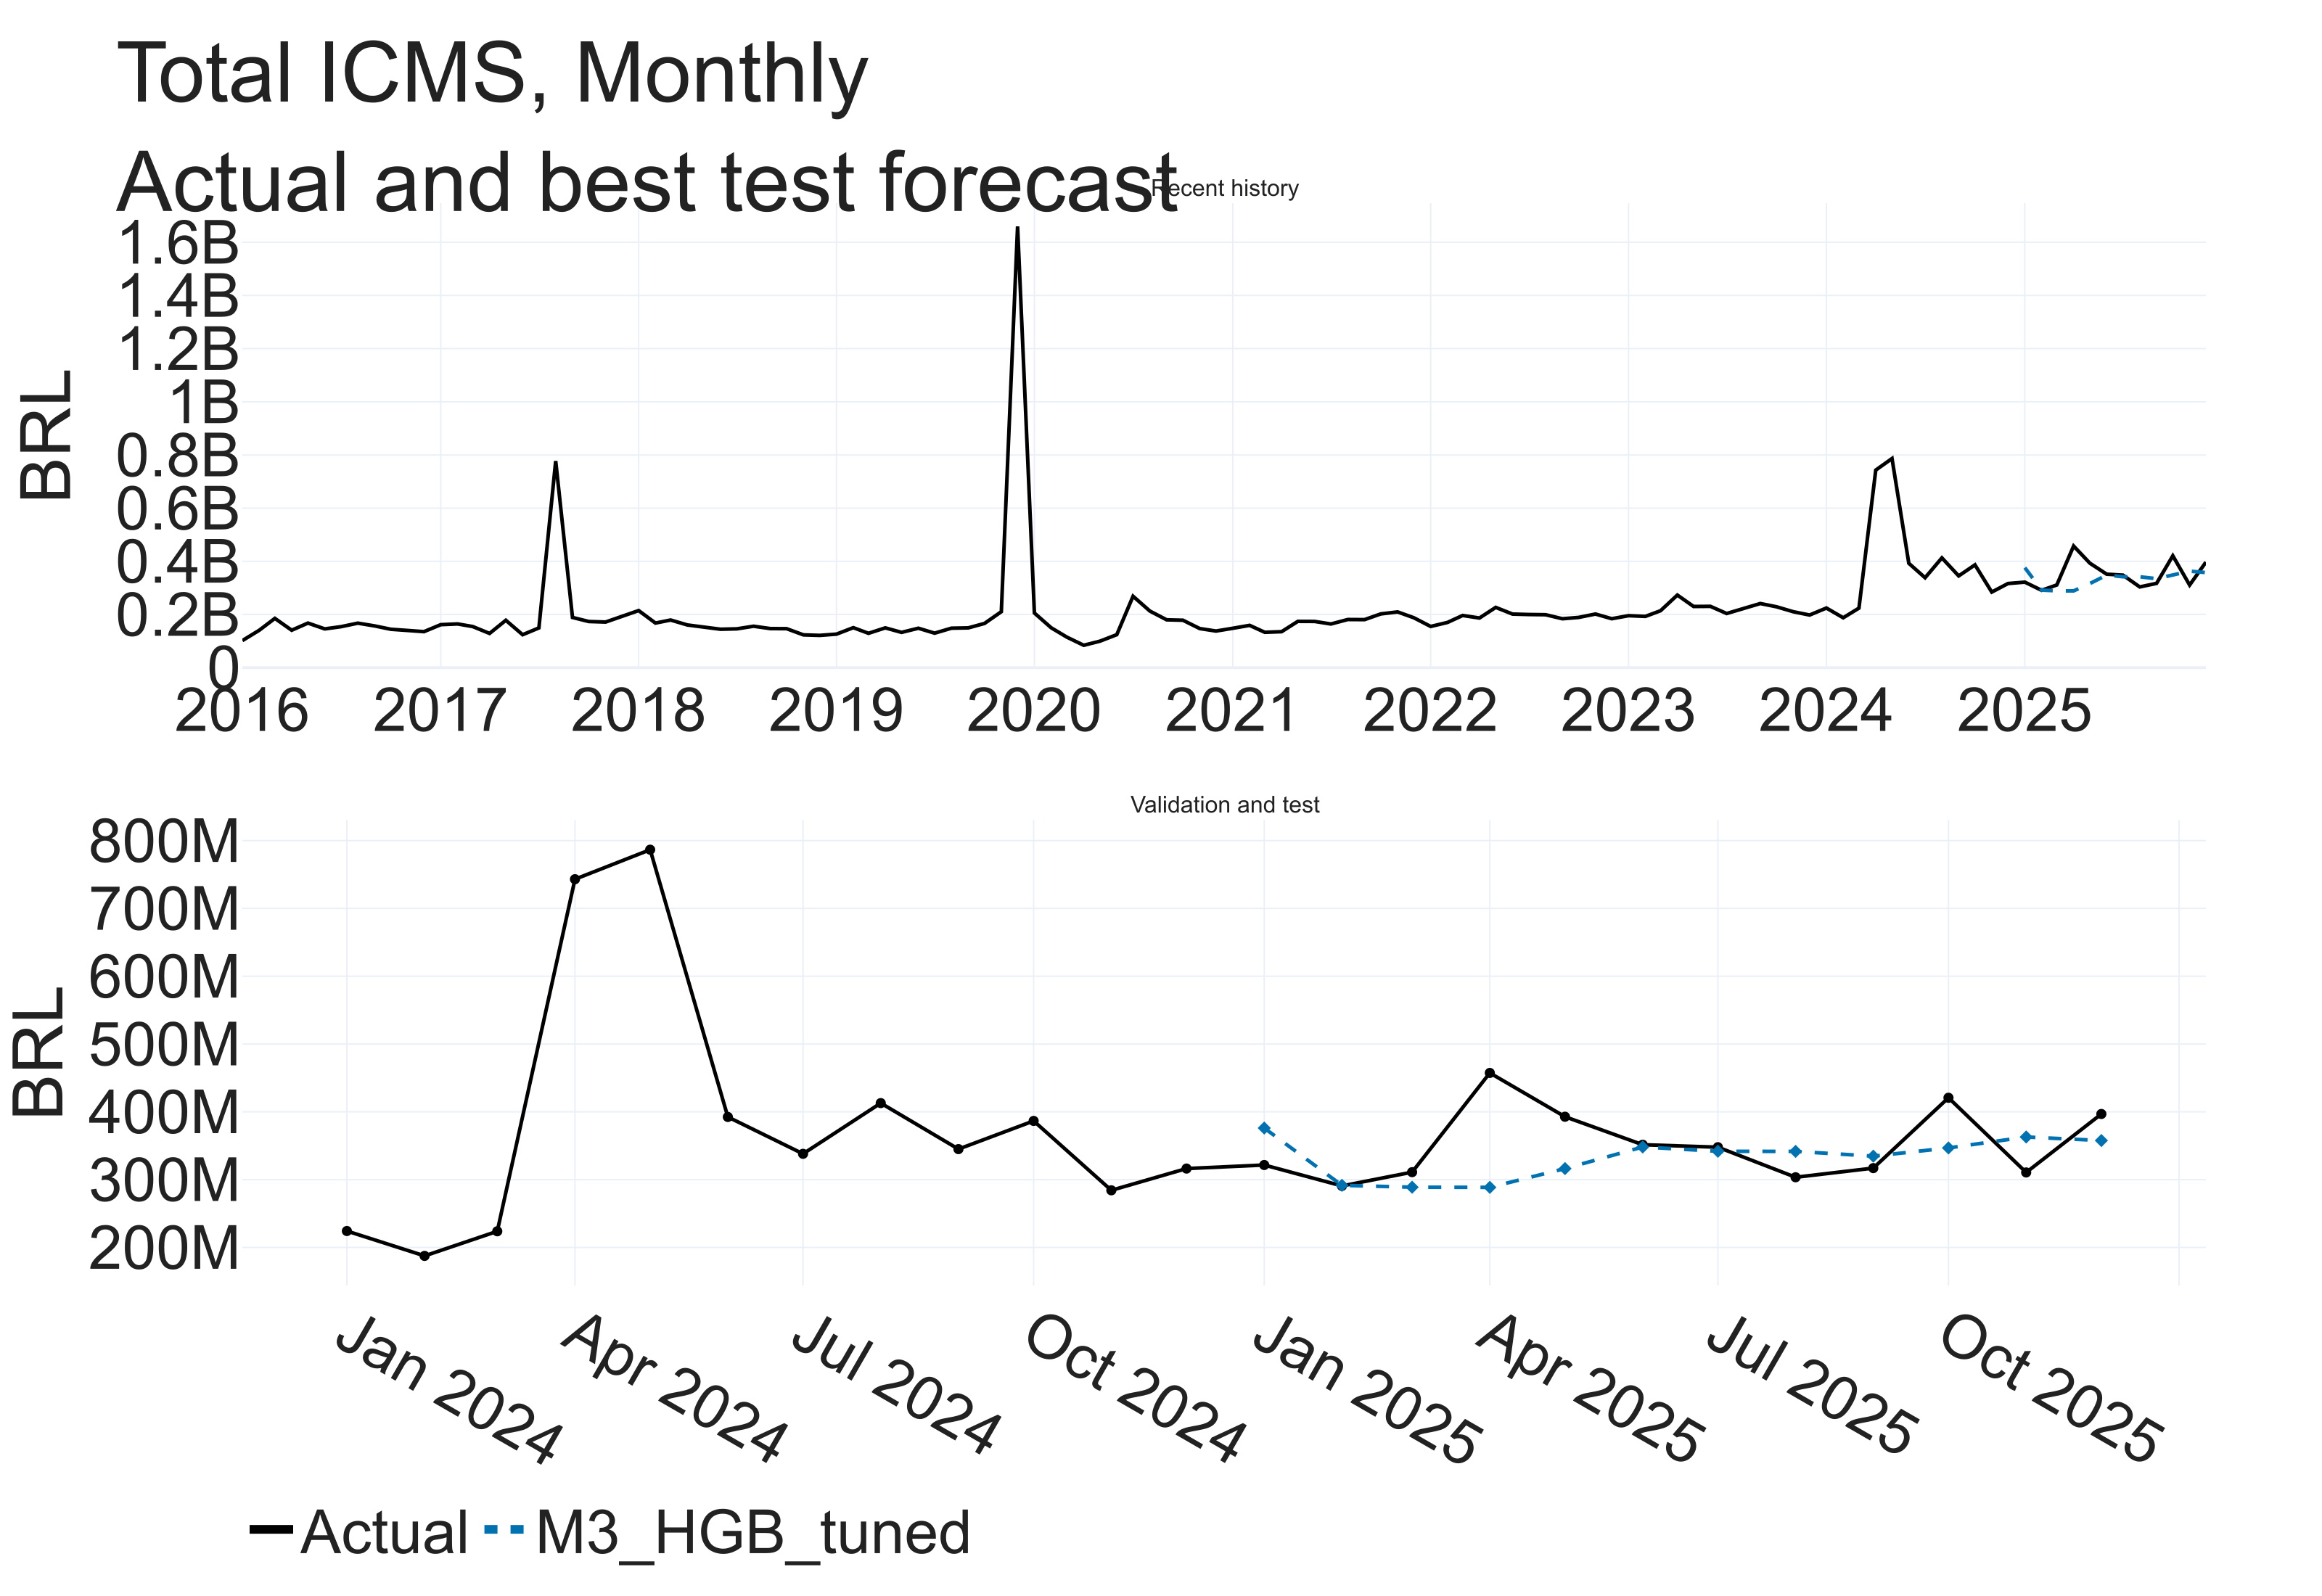
\includegraphics[width=\linewidth]{figures/segment/total_monthly_forecast.png}
  \caption{Total VAT (ICMS), monthly grain.
  Upper panel: history.
  Lower panel: validation and test.
  Black: actual.
  Blue dashed: M3 boosting on the test block.}
  \label{fig:m-total}
\end{figure}

\begin{figure}[H]
  \centering
  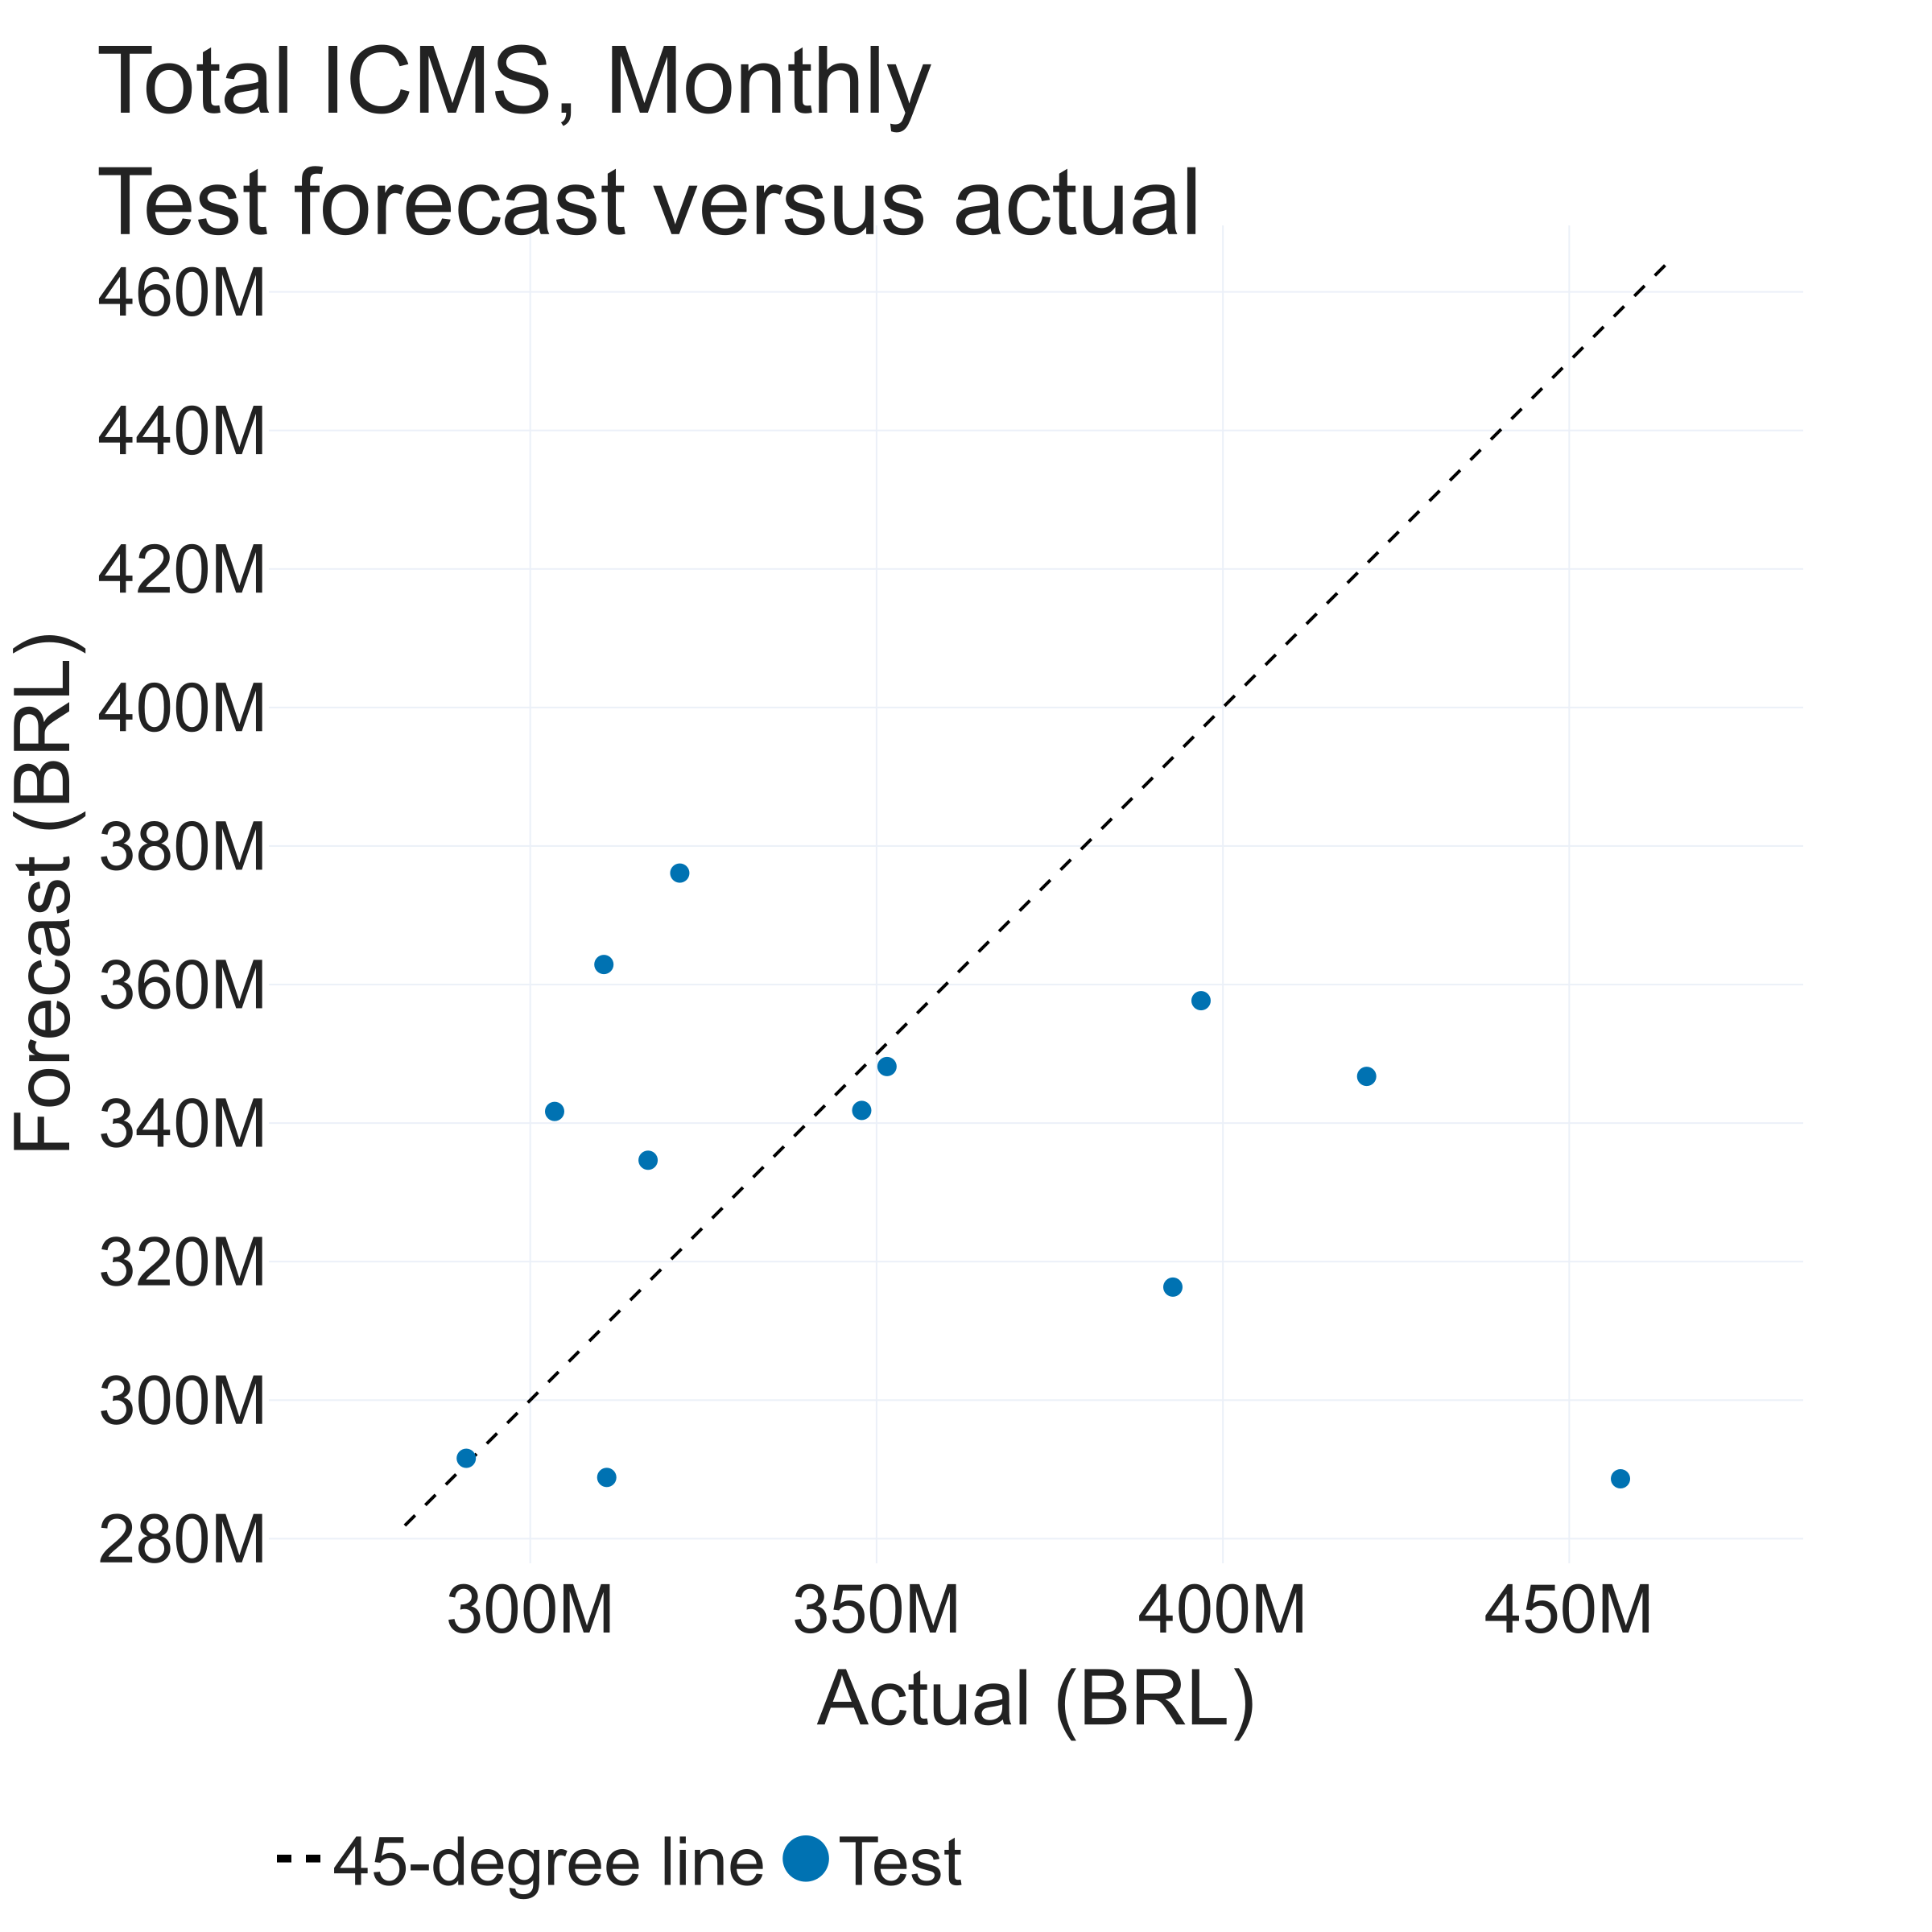
\includegraphics[width=0.72\linewidth]{figures/segment/total_monthly_scatter.png}
  \caption{Total VAT (ICMS), monthly test block.
  Horizontal axis: actual.
  Vertical axis: M3 boosting forecast.
  Dashed line: 45-degree line.}
  \label{fig:s-total}
\end{figure}

\begin{figure}[H]
  \centering
  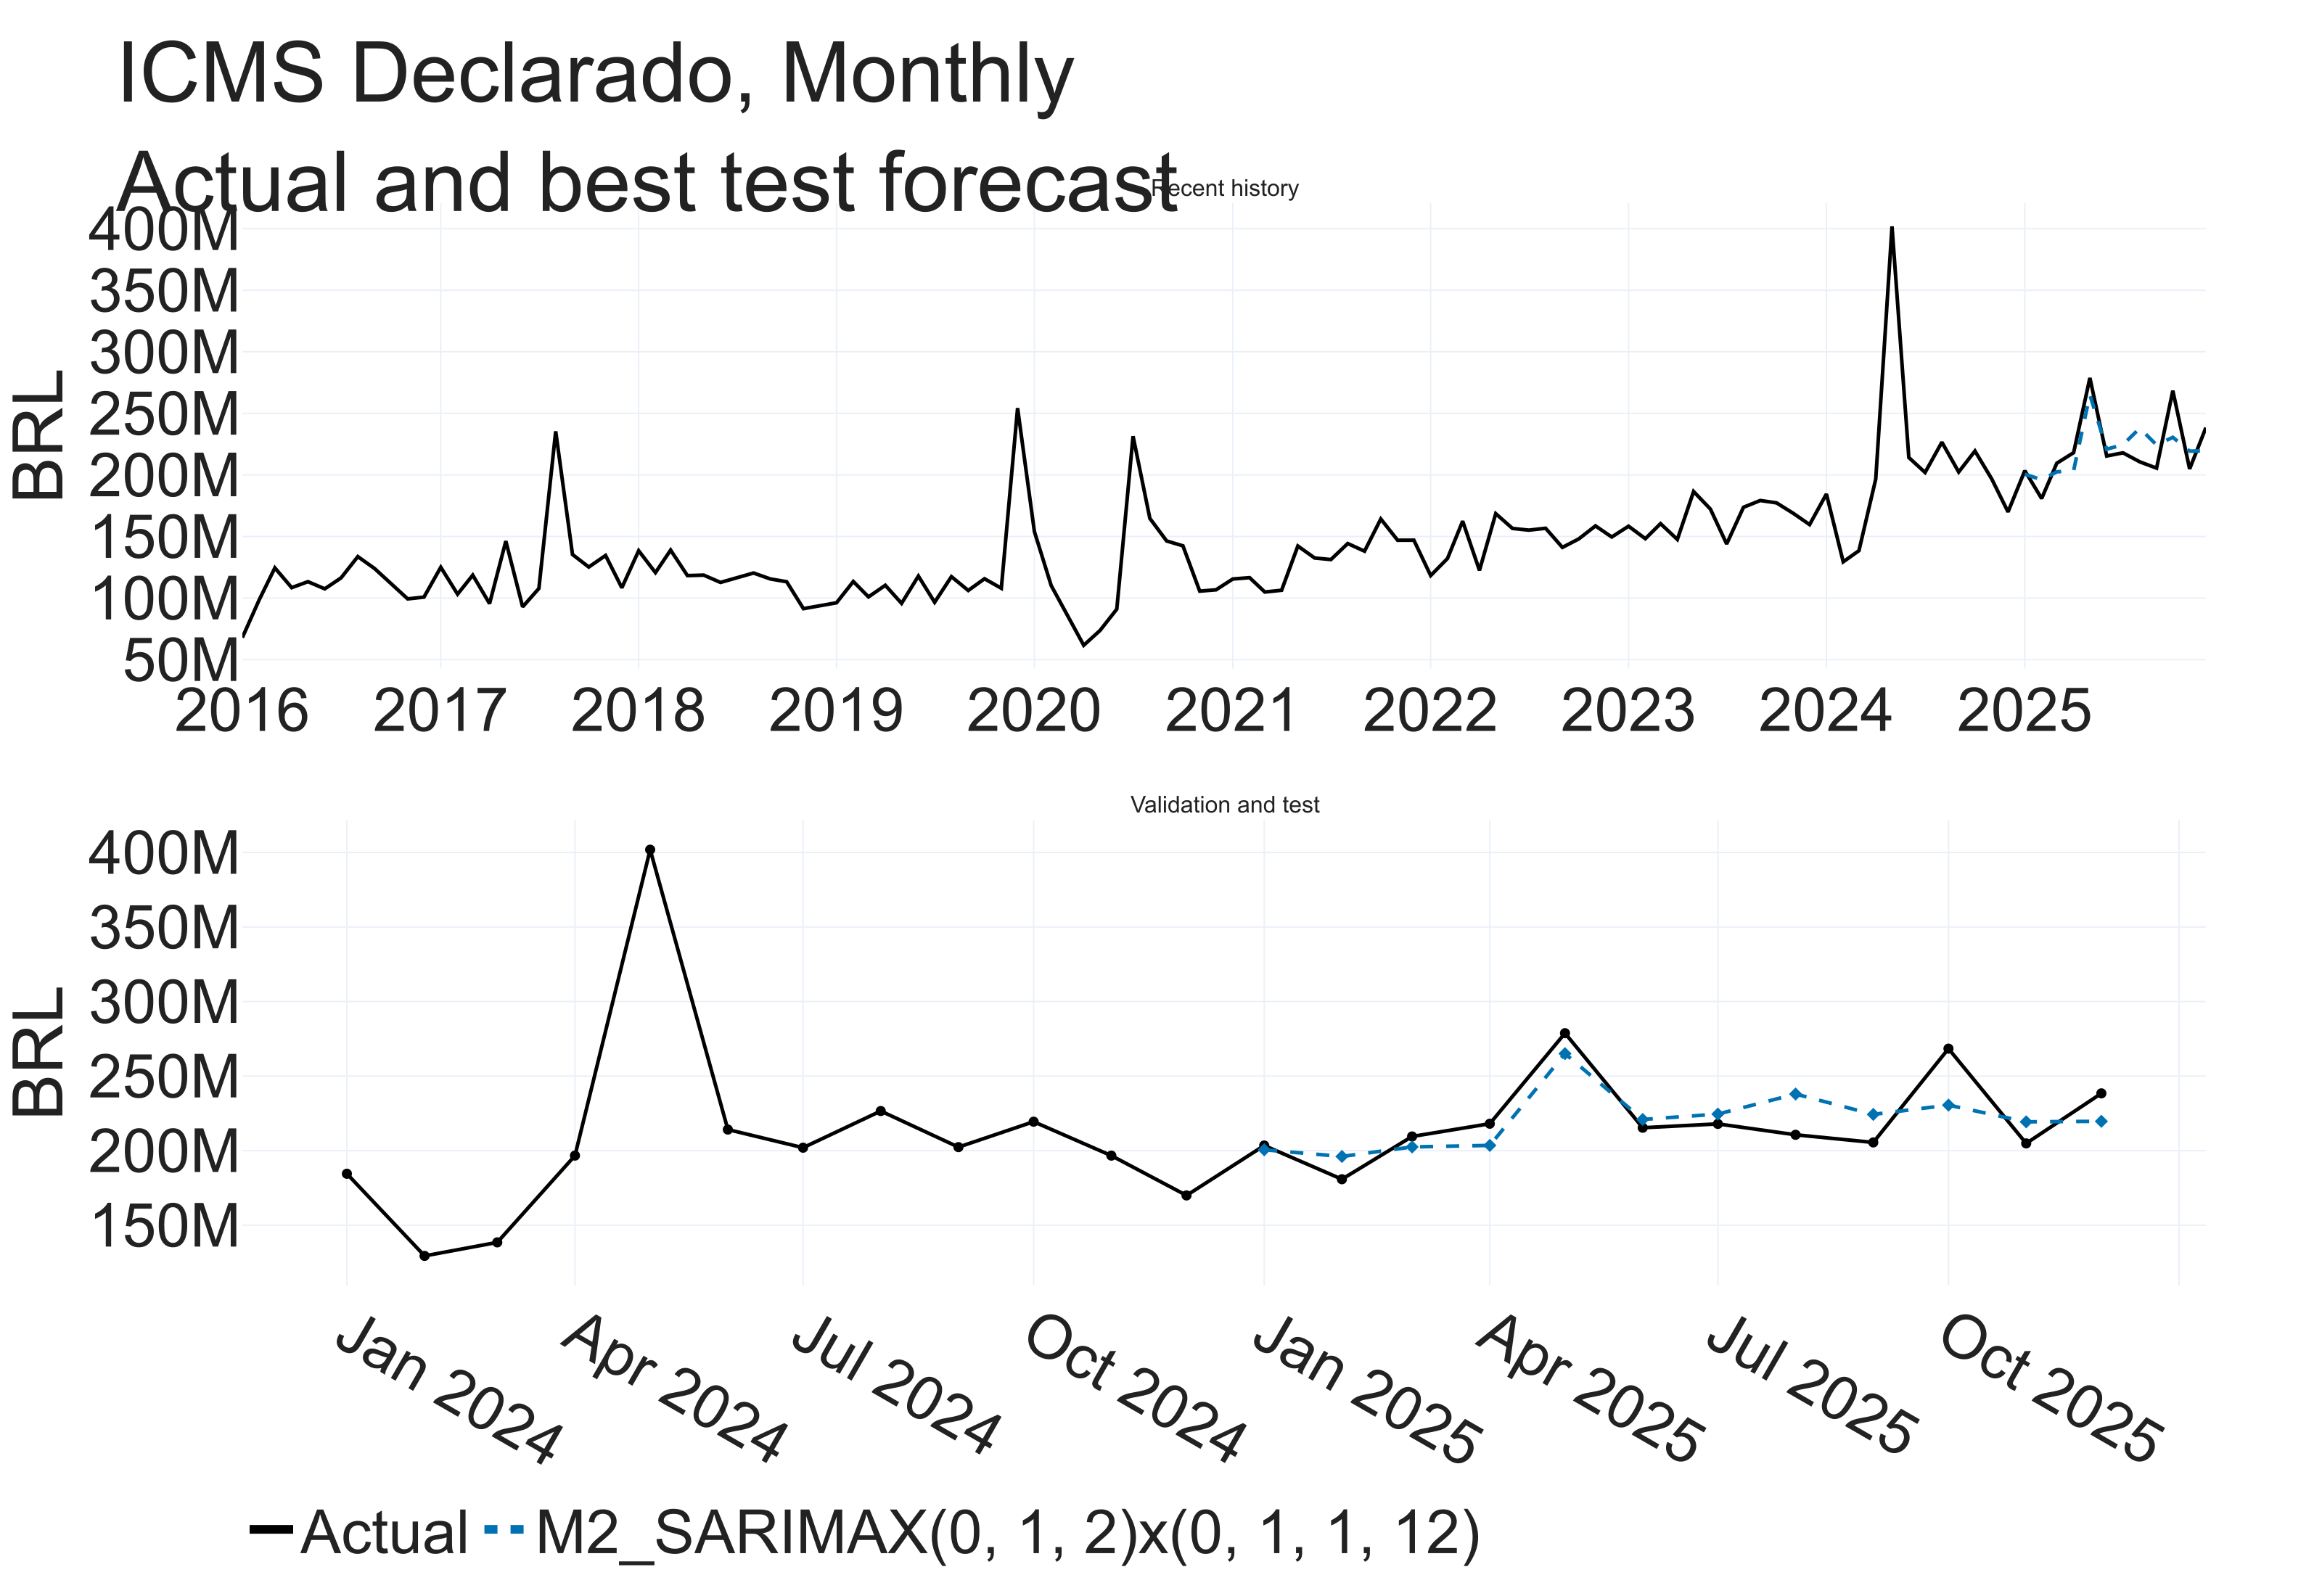
\includegraphics[width=\linewidth]{figures/segment/declarado_monthly_forecast.png}
  \caption{Declarado, monthly grain.
  Blue dashed: M2 SARIMAX on the test block.}
  \label{fig:m-dec}
\end{figure}

\begin{figure}[H]
  \centering
  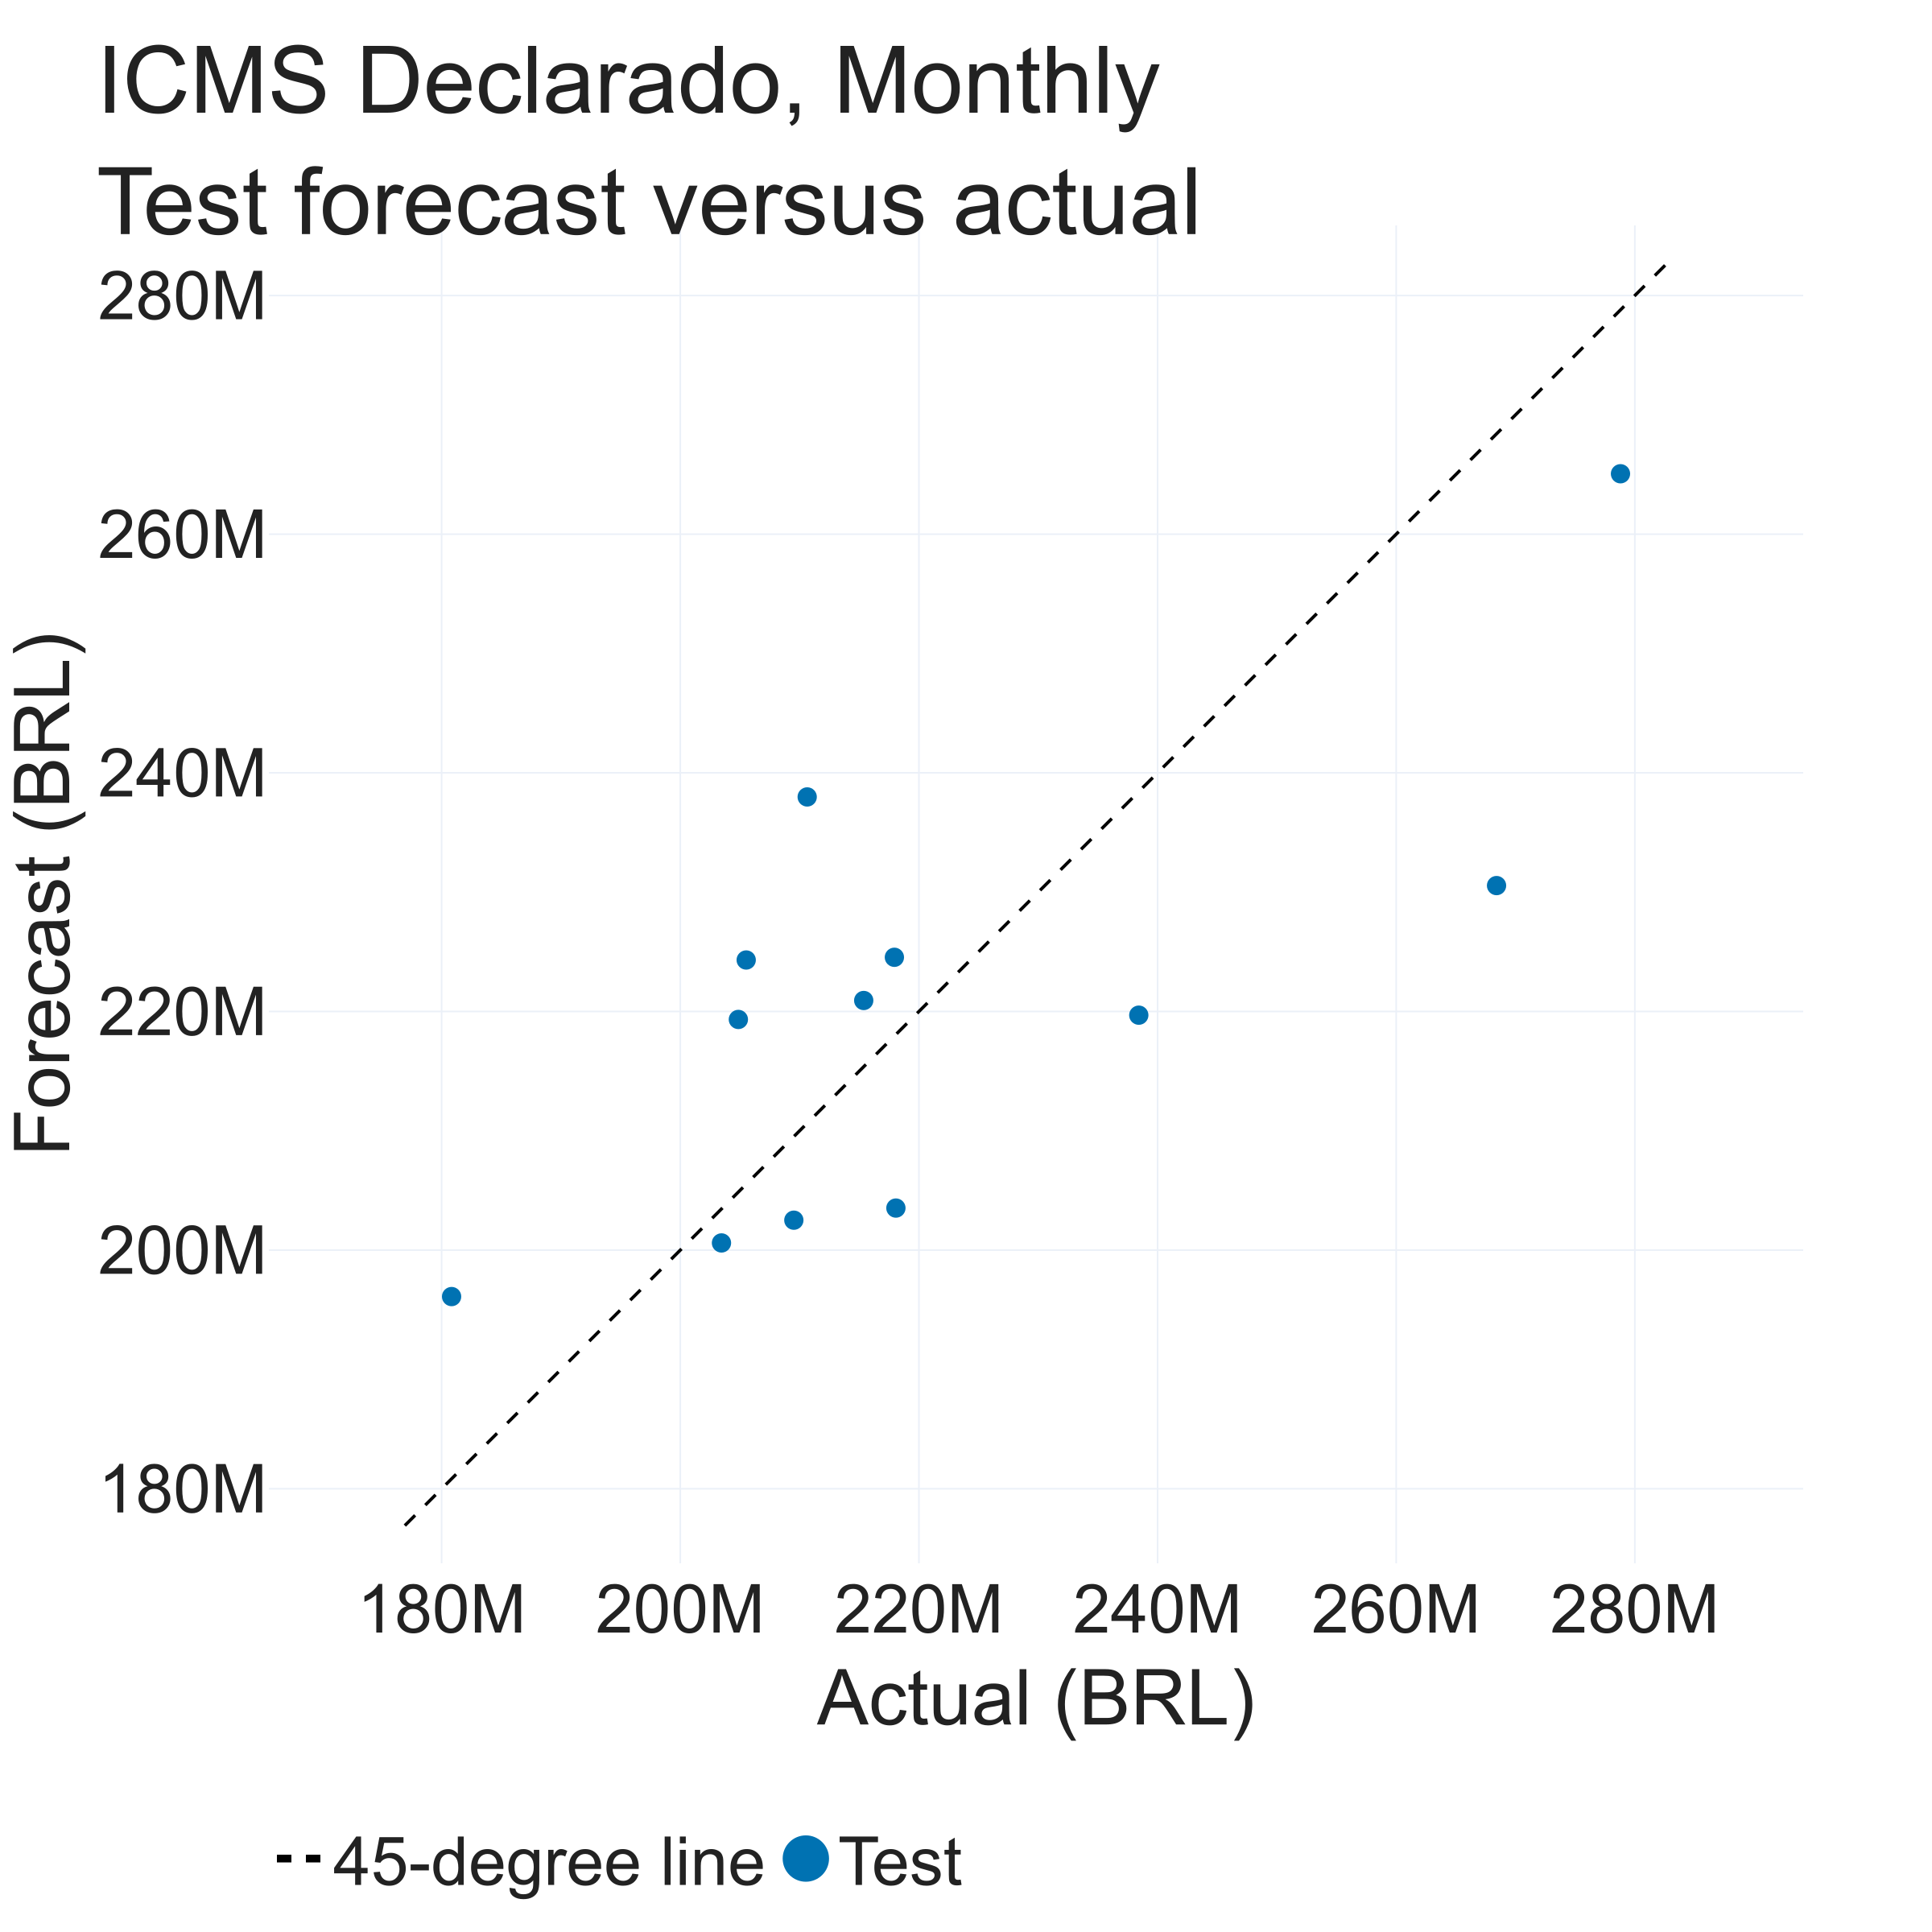
\includegraphics[width=0.72\linewidth]{figures/segment/declarado_monthly_scatter.png}
  \caption{Declarado, monthly test block.
  Dashed line: 45-degree line.}
  \label{fig:s-dec}
\end{figure}

\begin{figure}[H]
  \centering
  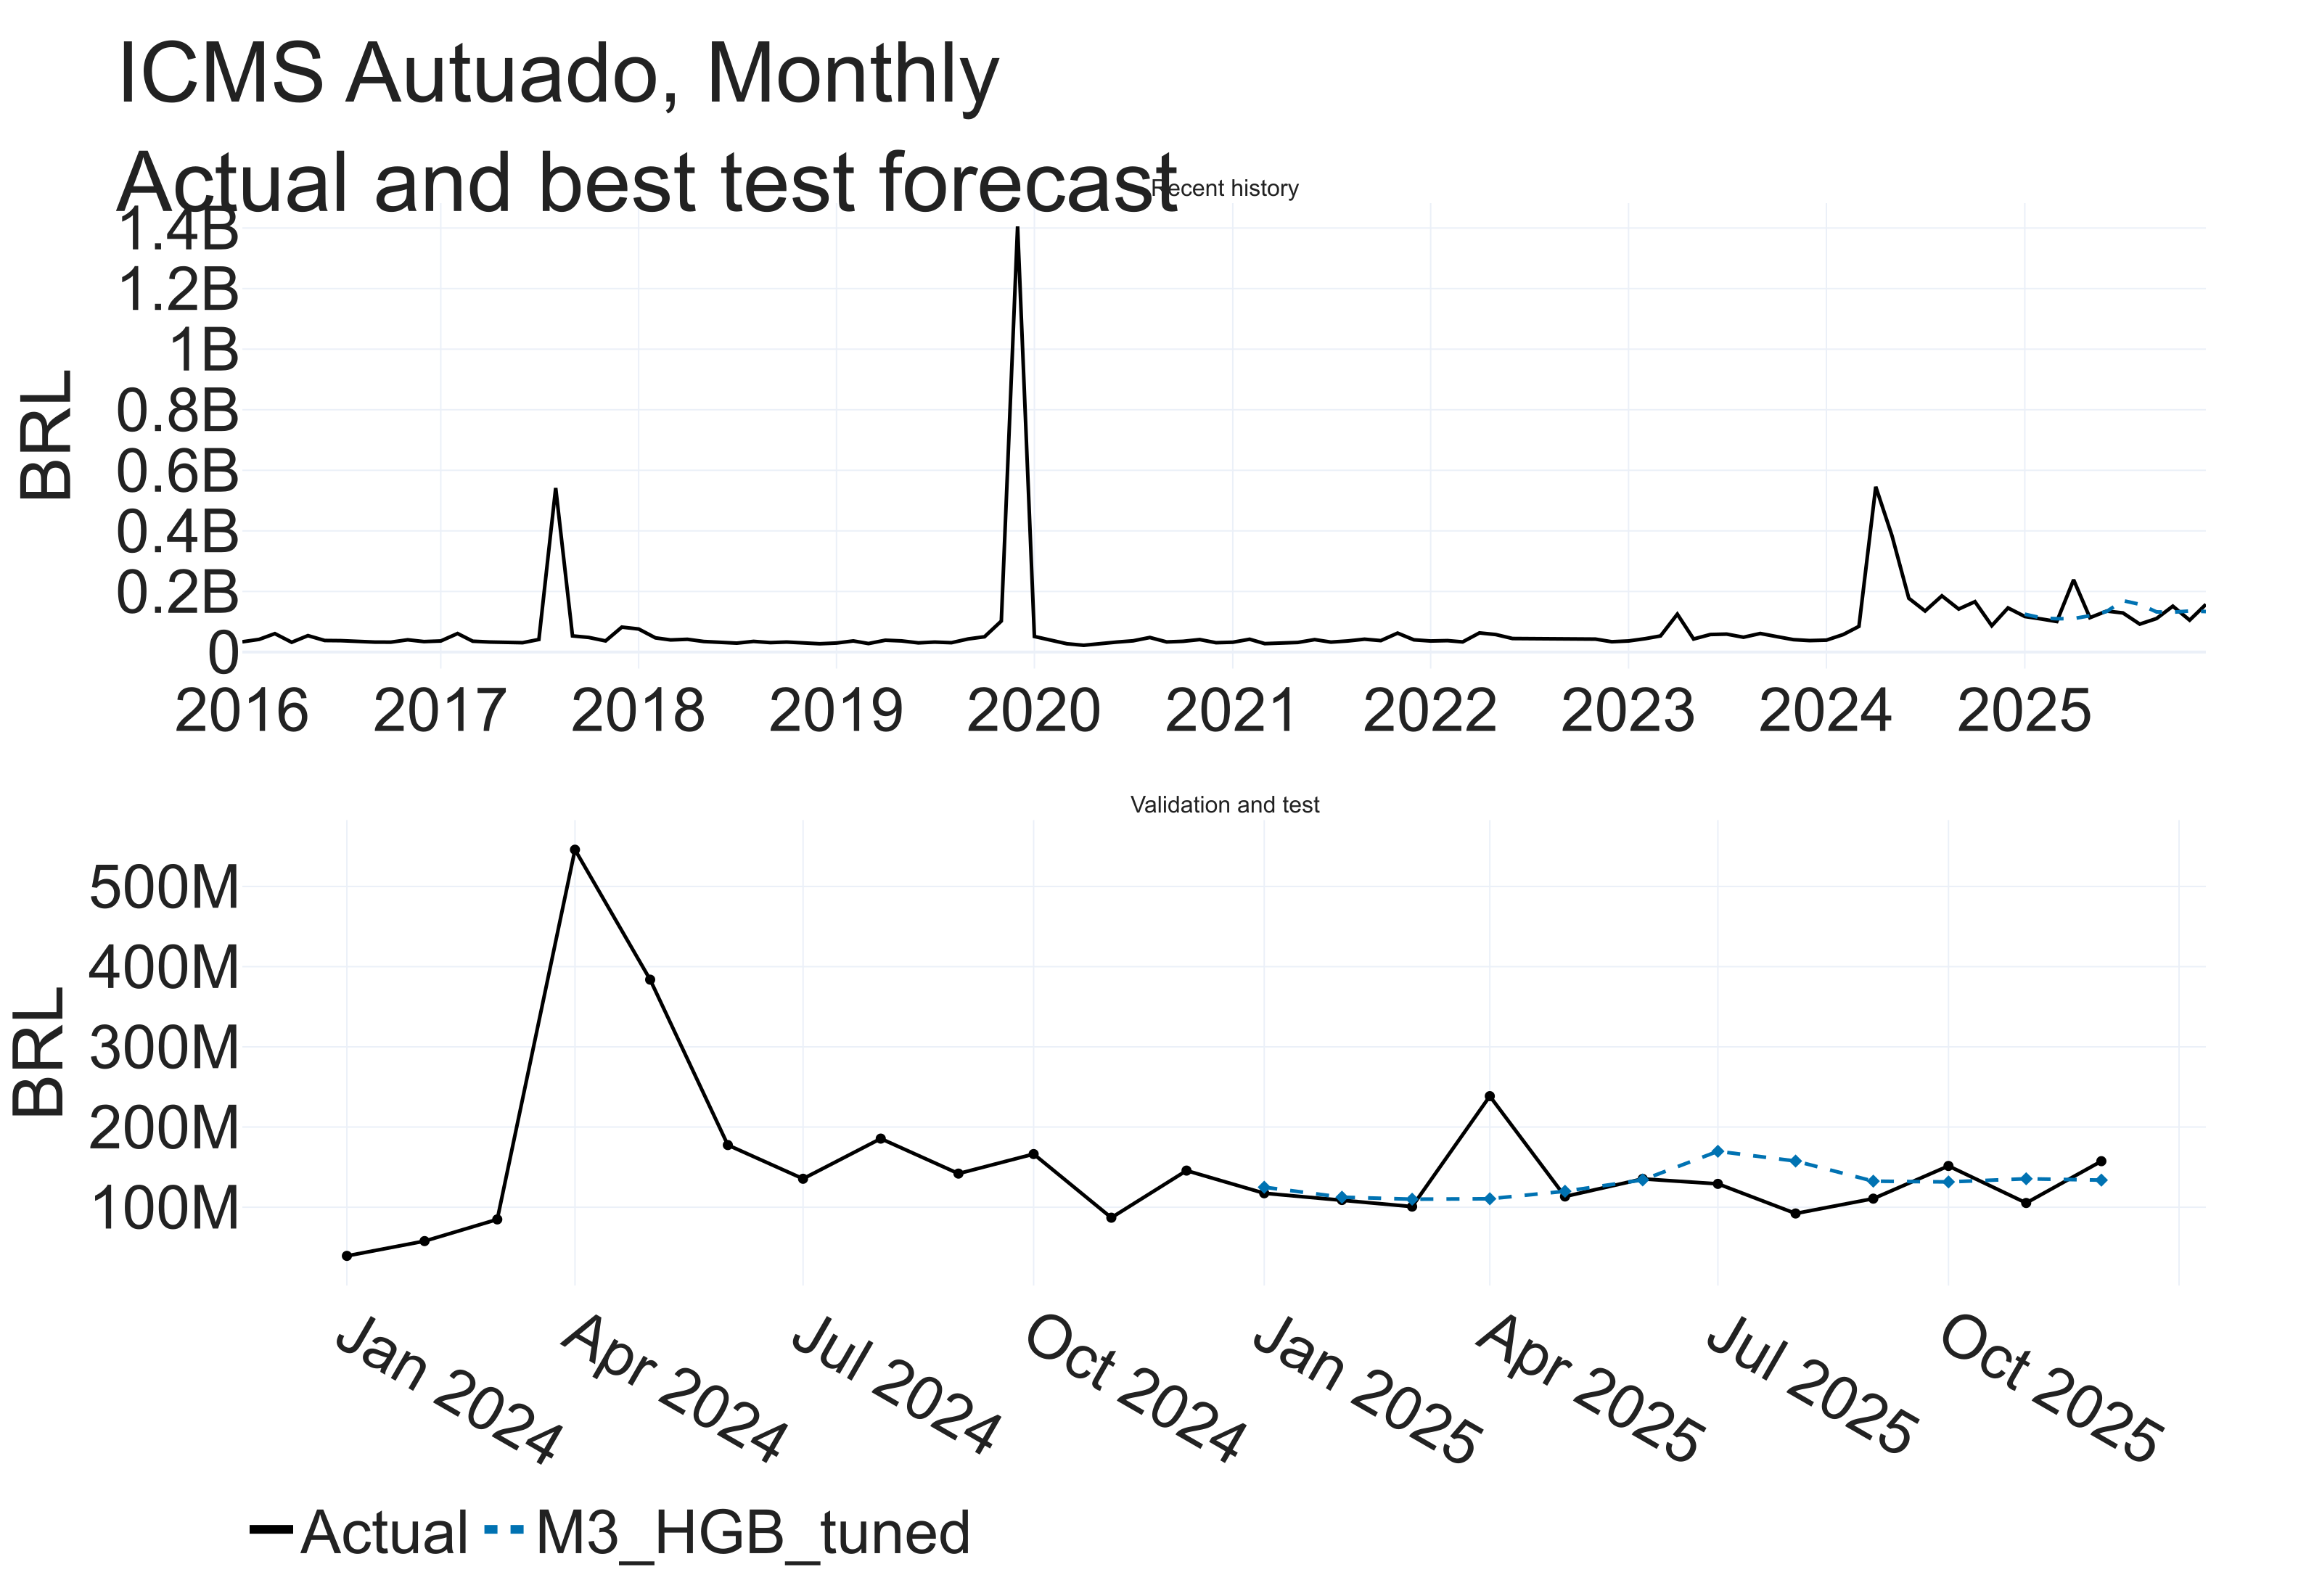
\includegraphics[width=\linewidth]{figures/segment/autuado_monthly_forecast.png}
  \caption{Autuado, monthly grain.
  Blue dashed: M3 boosting on the test block.}
  \label{fig:m-aut}
\end{figure}

\begin{figure}[H]
  \centering
  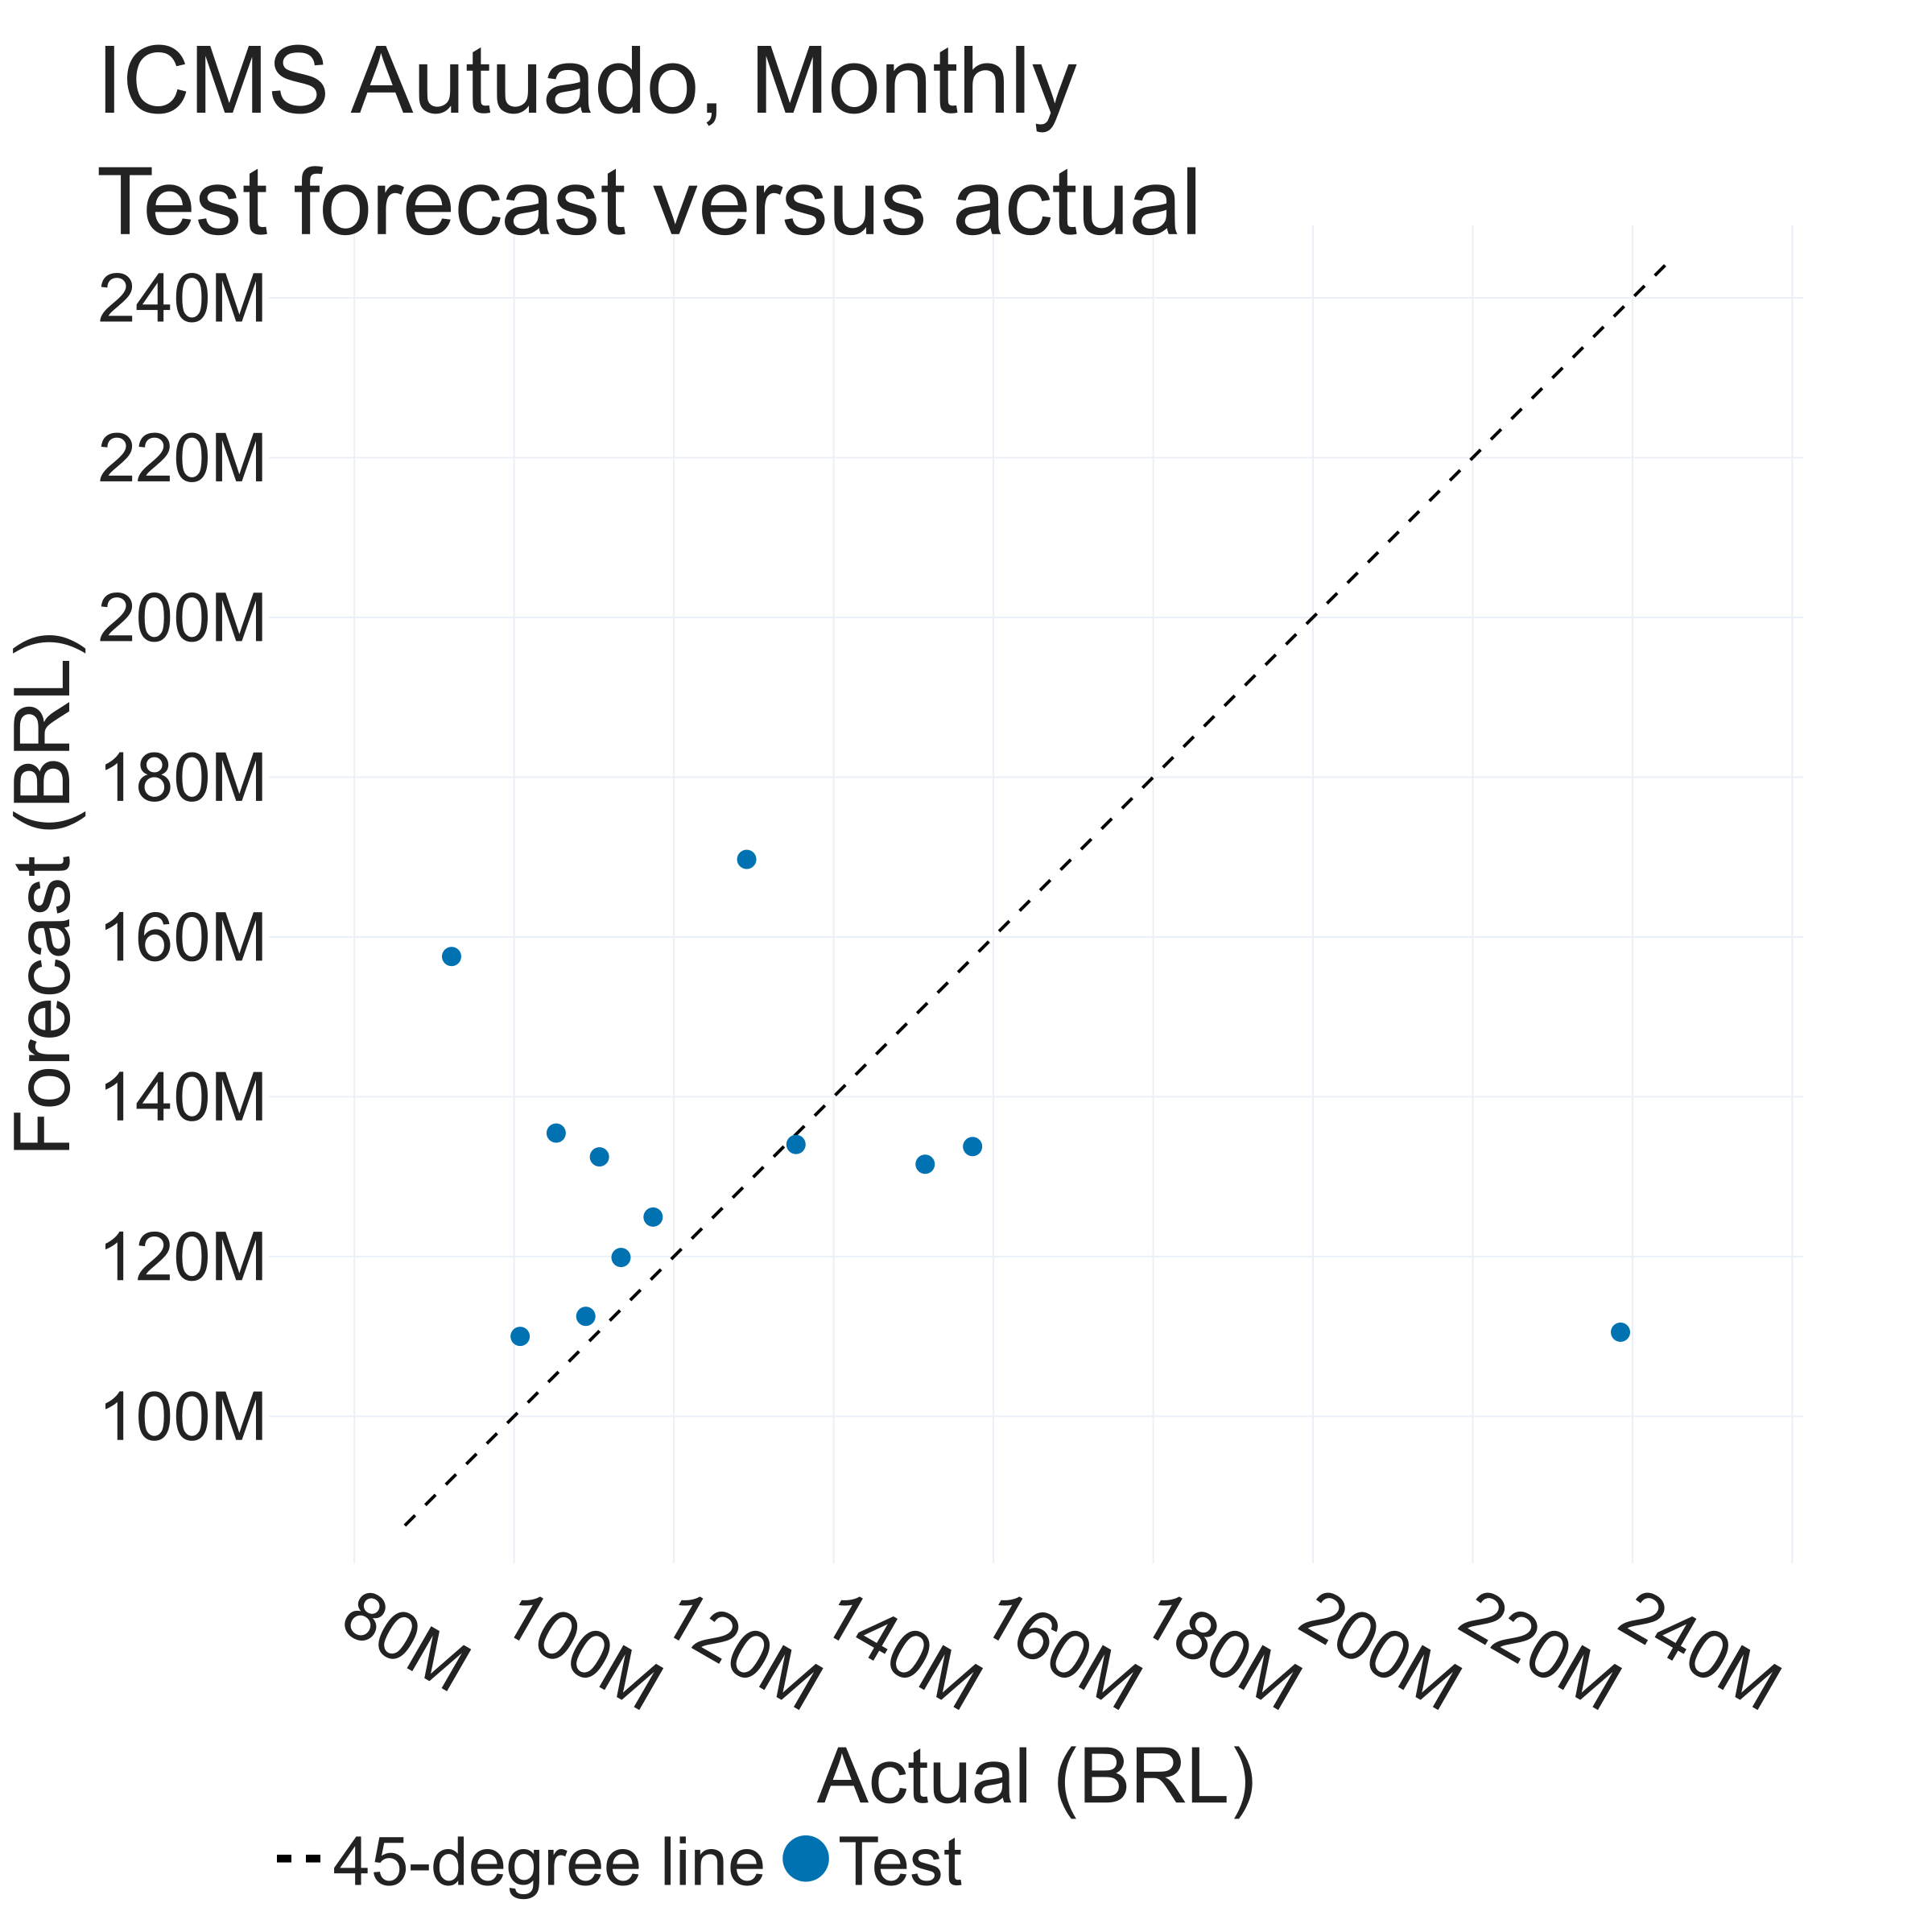
\includegraphics[width=0.72\linewidth]{figures/segment/autuado_monthly_scatter.png}
  \caption{Autuado, monthly test block.
  Dashed line: 45-degree line.}
  \label{fig:s-aut}
\end{figure}

\section{Conclusion}
\label{sec:conclusion}

[DISCUTIR E ESCREVER]

\section{Limitations}
\label{sec:limitations}

\begin{itemize}
  \item The monthly test block has 12 points.
        The weekly test block has 13 points.
        A model confidence set on those blocks is wide.
  \item Each grain has one test window.
        The study does not use a rolling origin.
  \item Grain B keeps holidays and has no holiday indicator.
  \item E1 did not run.
        The TEM vendor tree is absent.
        The tables do not contain an E1 score.
  \item sMAPE on a series with many zero days is hard to read as an operational error.
        The rank still uses every day in grain A, including zeros.
  \item The skill score uses the Murphy ratio on sMAPE~\citep{murphy1988skill}.
        It compares a model only with the seasonal naive of the same grain.
  \item A low sMAPE can still miss the peaks.
        On the monthly total, boosting leads and the month-to-month order is weak.
        Read the scatter next to the rank.
  \item The HLN test compares the leader with the seasonal naive only.
        It does not compare the leader with the second-best model.
  \item The HLN test in this paper uses horizon 1.
        Some models forecast the whole test block from one origin.
        Their errors are dependent.
        The p-value is a paired comparison of the stored losses, not a multi-step correction with \(h\) equal to the test length.
        That correction is not positive when \(h\) equals the test length.
\end{itemize}


\appendix
\section{Other grains}
\label{app:figures}

The monthly charts are in Section~\ref{sec:discussion}.
This appendix holds the weekly grain, grain A, and grain B for the same three series.
Each time chart has a zoom on the validation block and the test block.
Each scatter is the test block and a 45-degree line.
The blue dashed line is the lowest-sMAPE model on that series and grain.

[DISCUTIR E ESCREVER]

\begin{figure}[H]
  \centering
  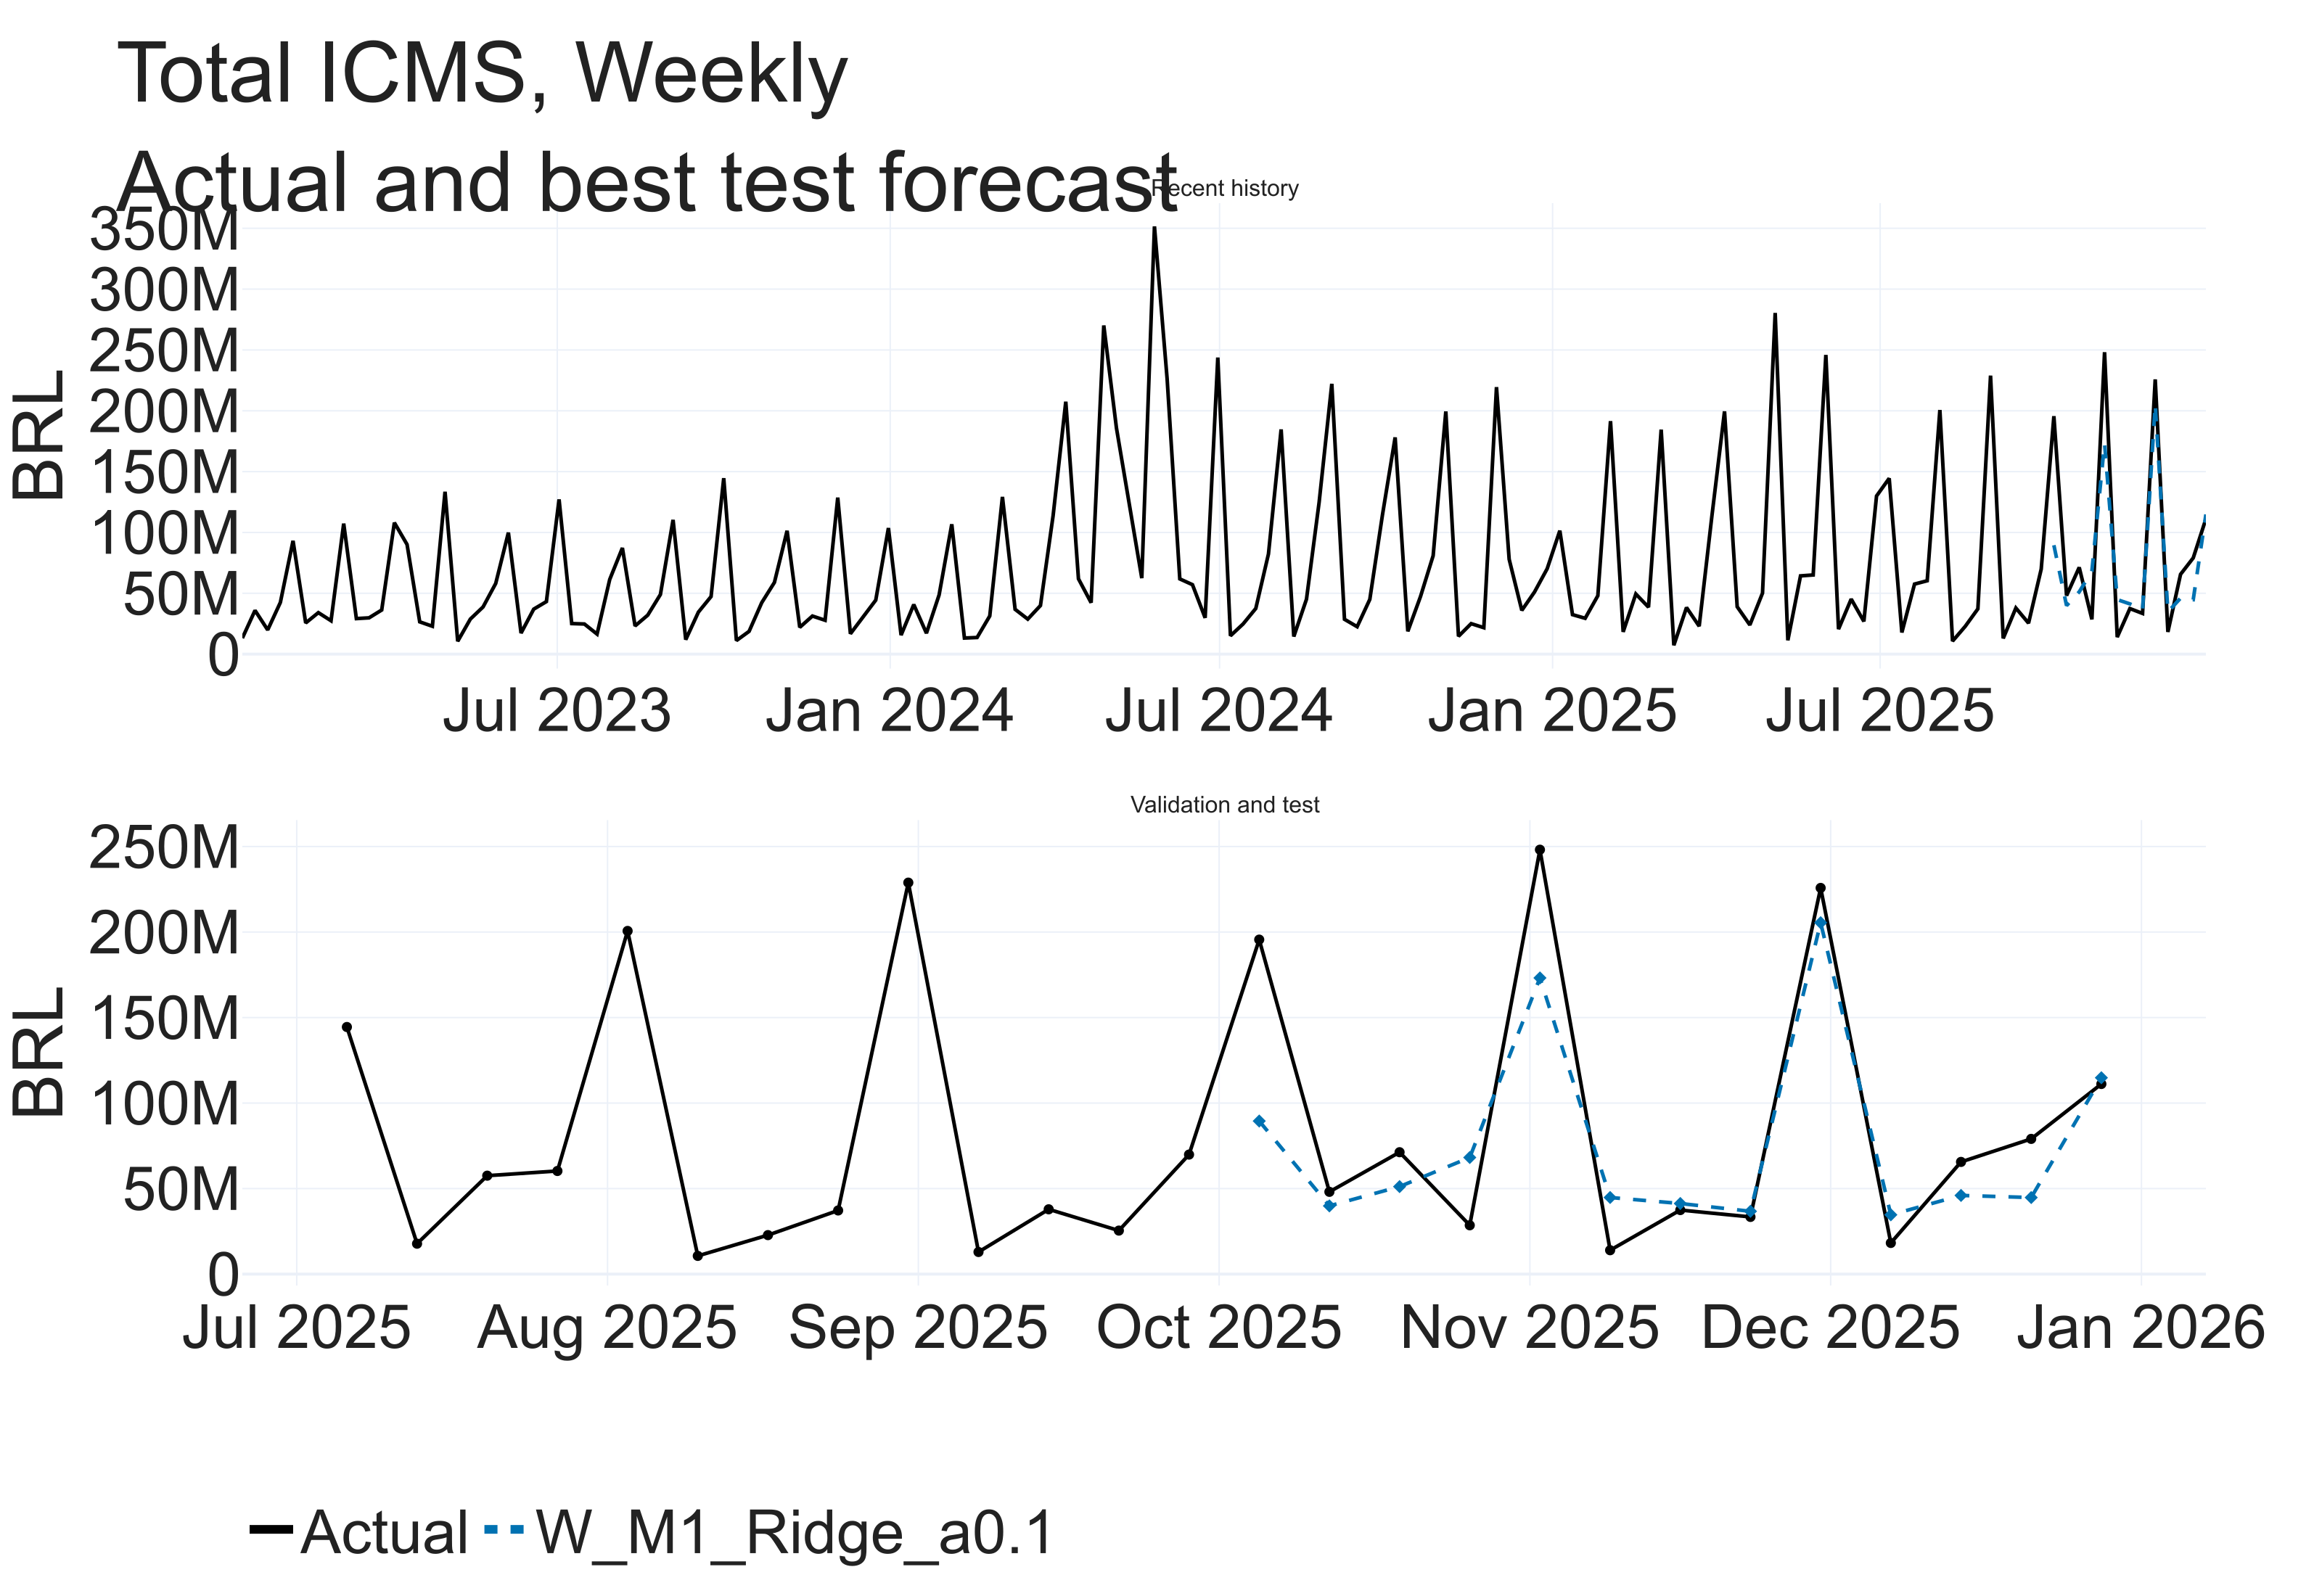
\includegraphics[width=\linewidth]{figures/segment/total_weekly_forecast.png}
  \caption{Total, weekly. Blue dashed: M1 ridge.}
\end{figure}
\begin{figure}[H]
  \centering
  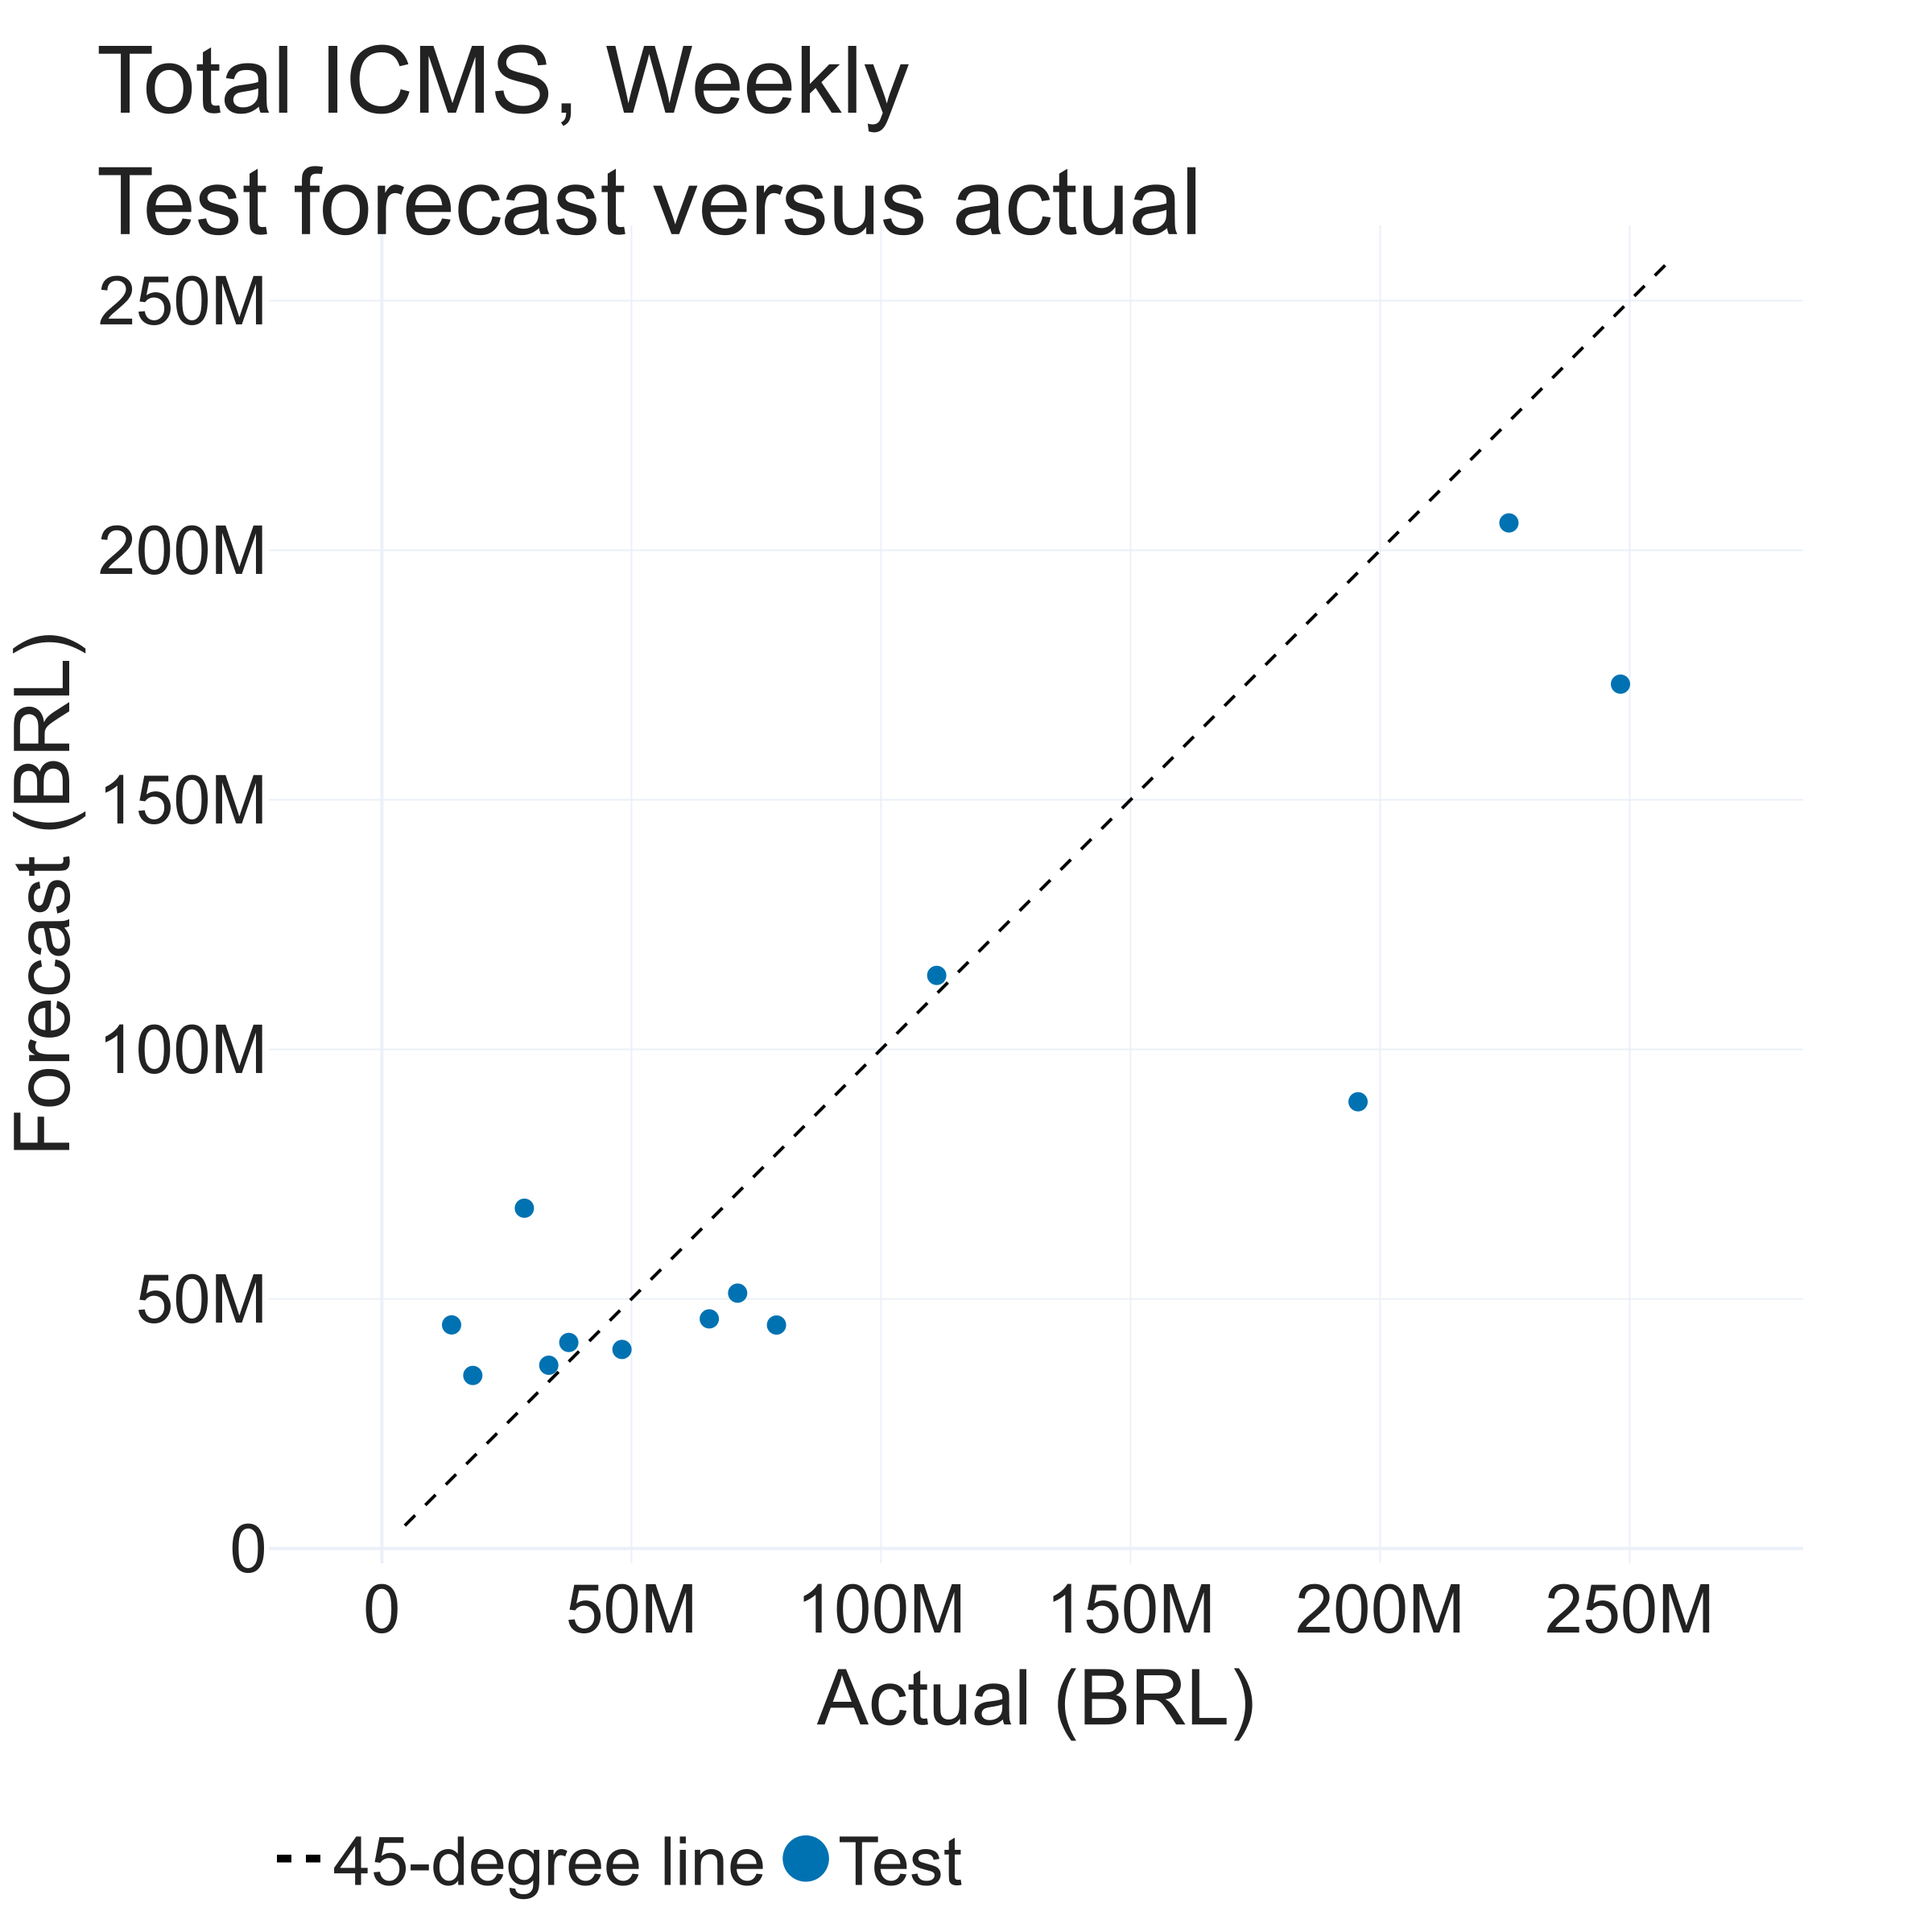
\includegraphics[width=0.62\linewidth]{figures/segment/total_weekly_scatter.png}
  \caption{Total, weekly test scatter.}
\end{figure}
\begin{figure}[H]
  \centering
  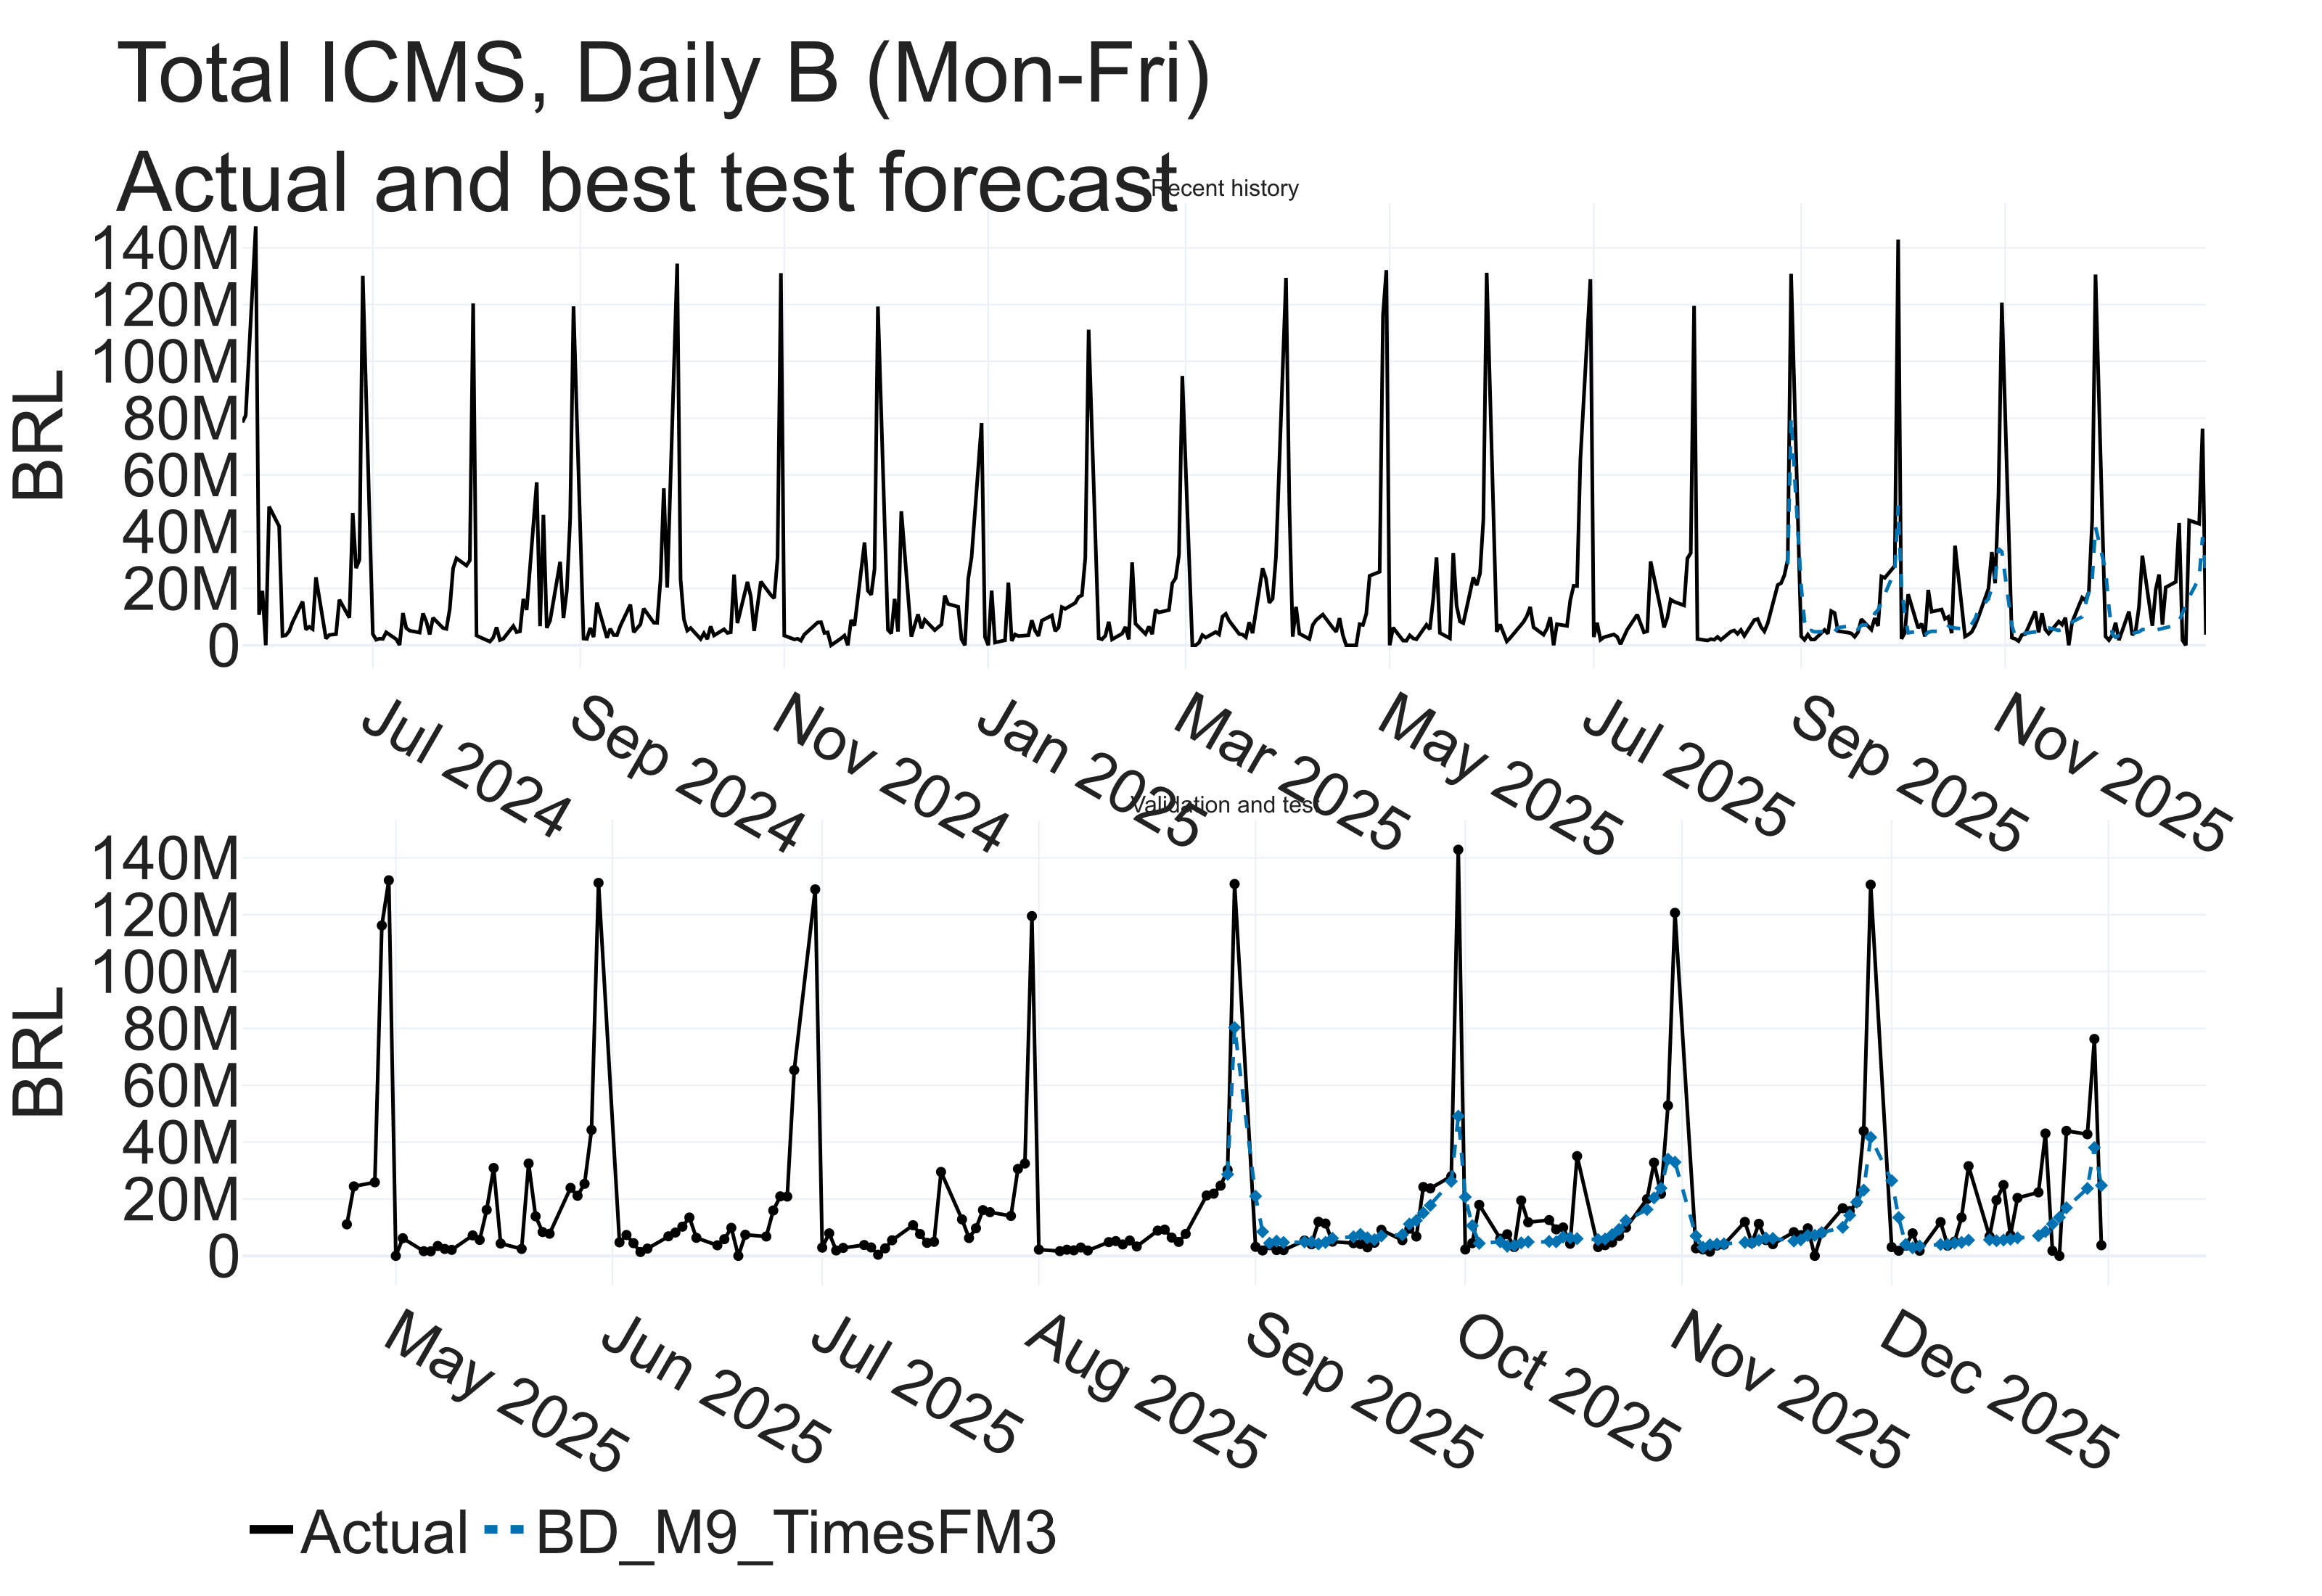
\includegraphics[width=\linewidth]{figures/segment/total_business_daily_forecast.png}
  \caption{Total, daily B. Blue dashed: M9 TimesFM.}
\end{figure}
\begin{figure}[H]
  \centering
  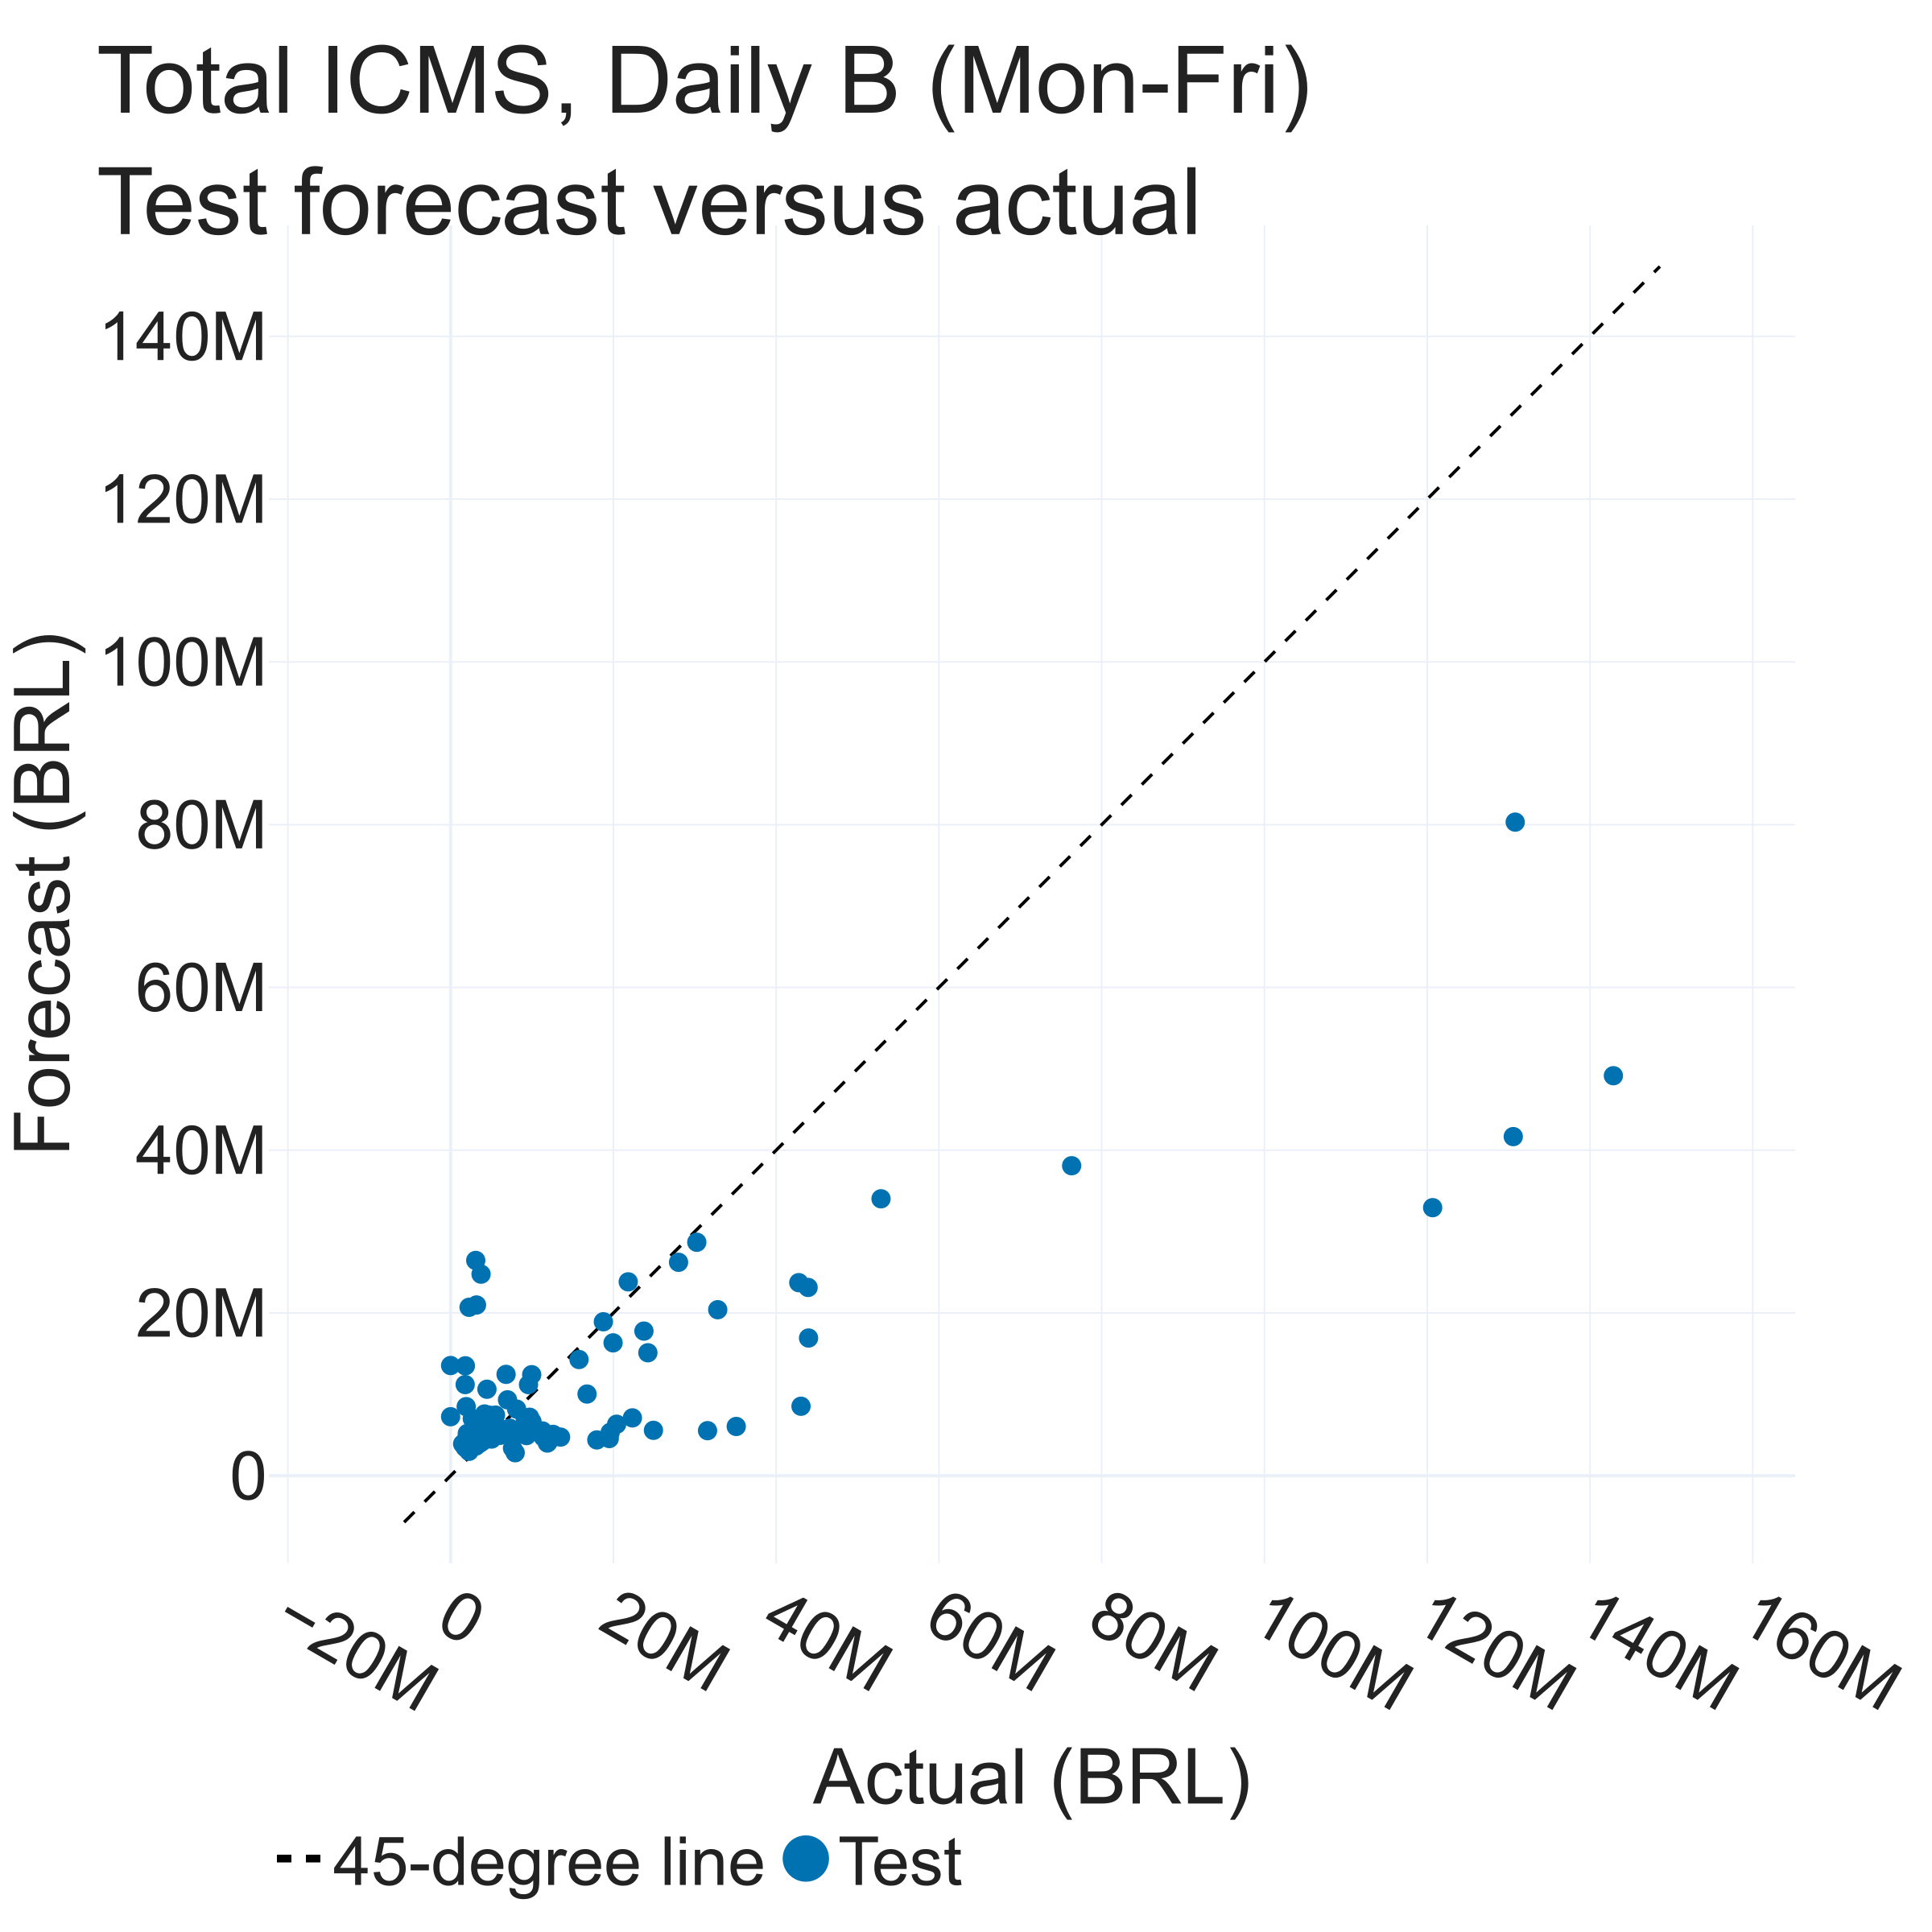
\includegraphics[width=0.62\linewidth]{figures/segment/total_business_daily_scatter.png}
  \caption{Total, daily B test scatter.}
\end{figure}
\begin{figure}[H]
  \centering
  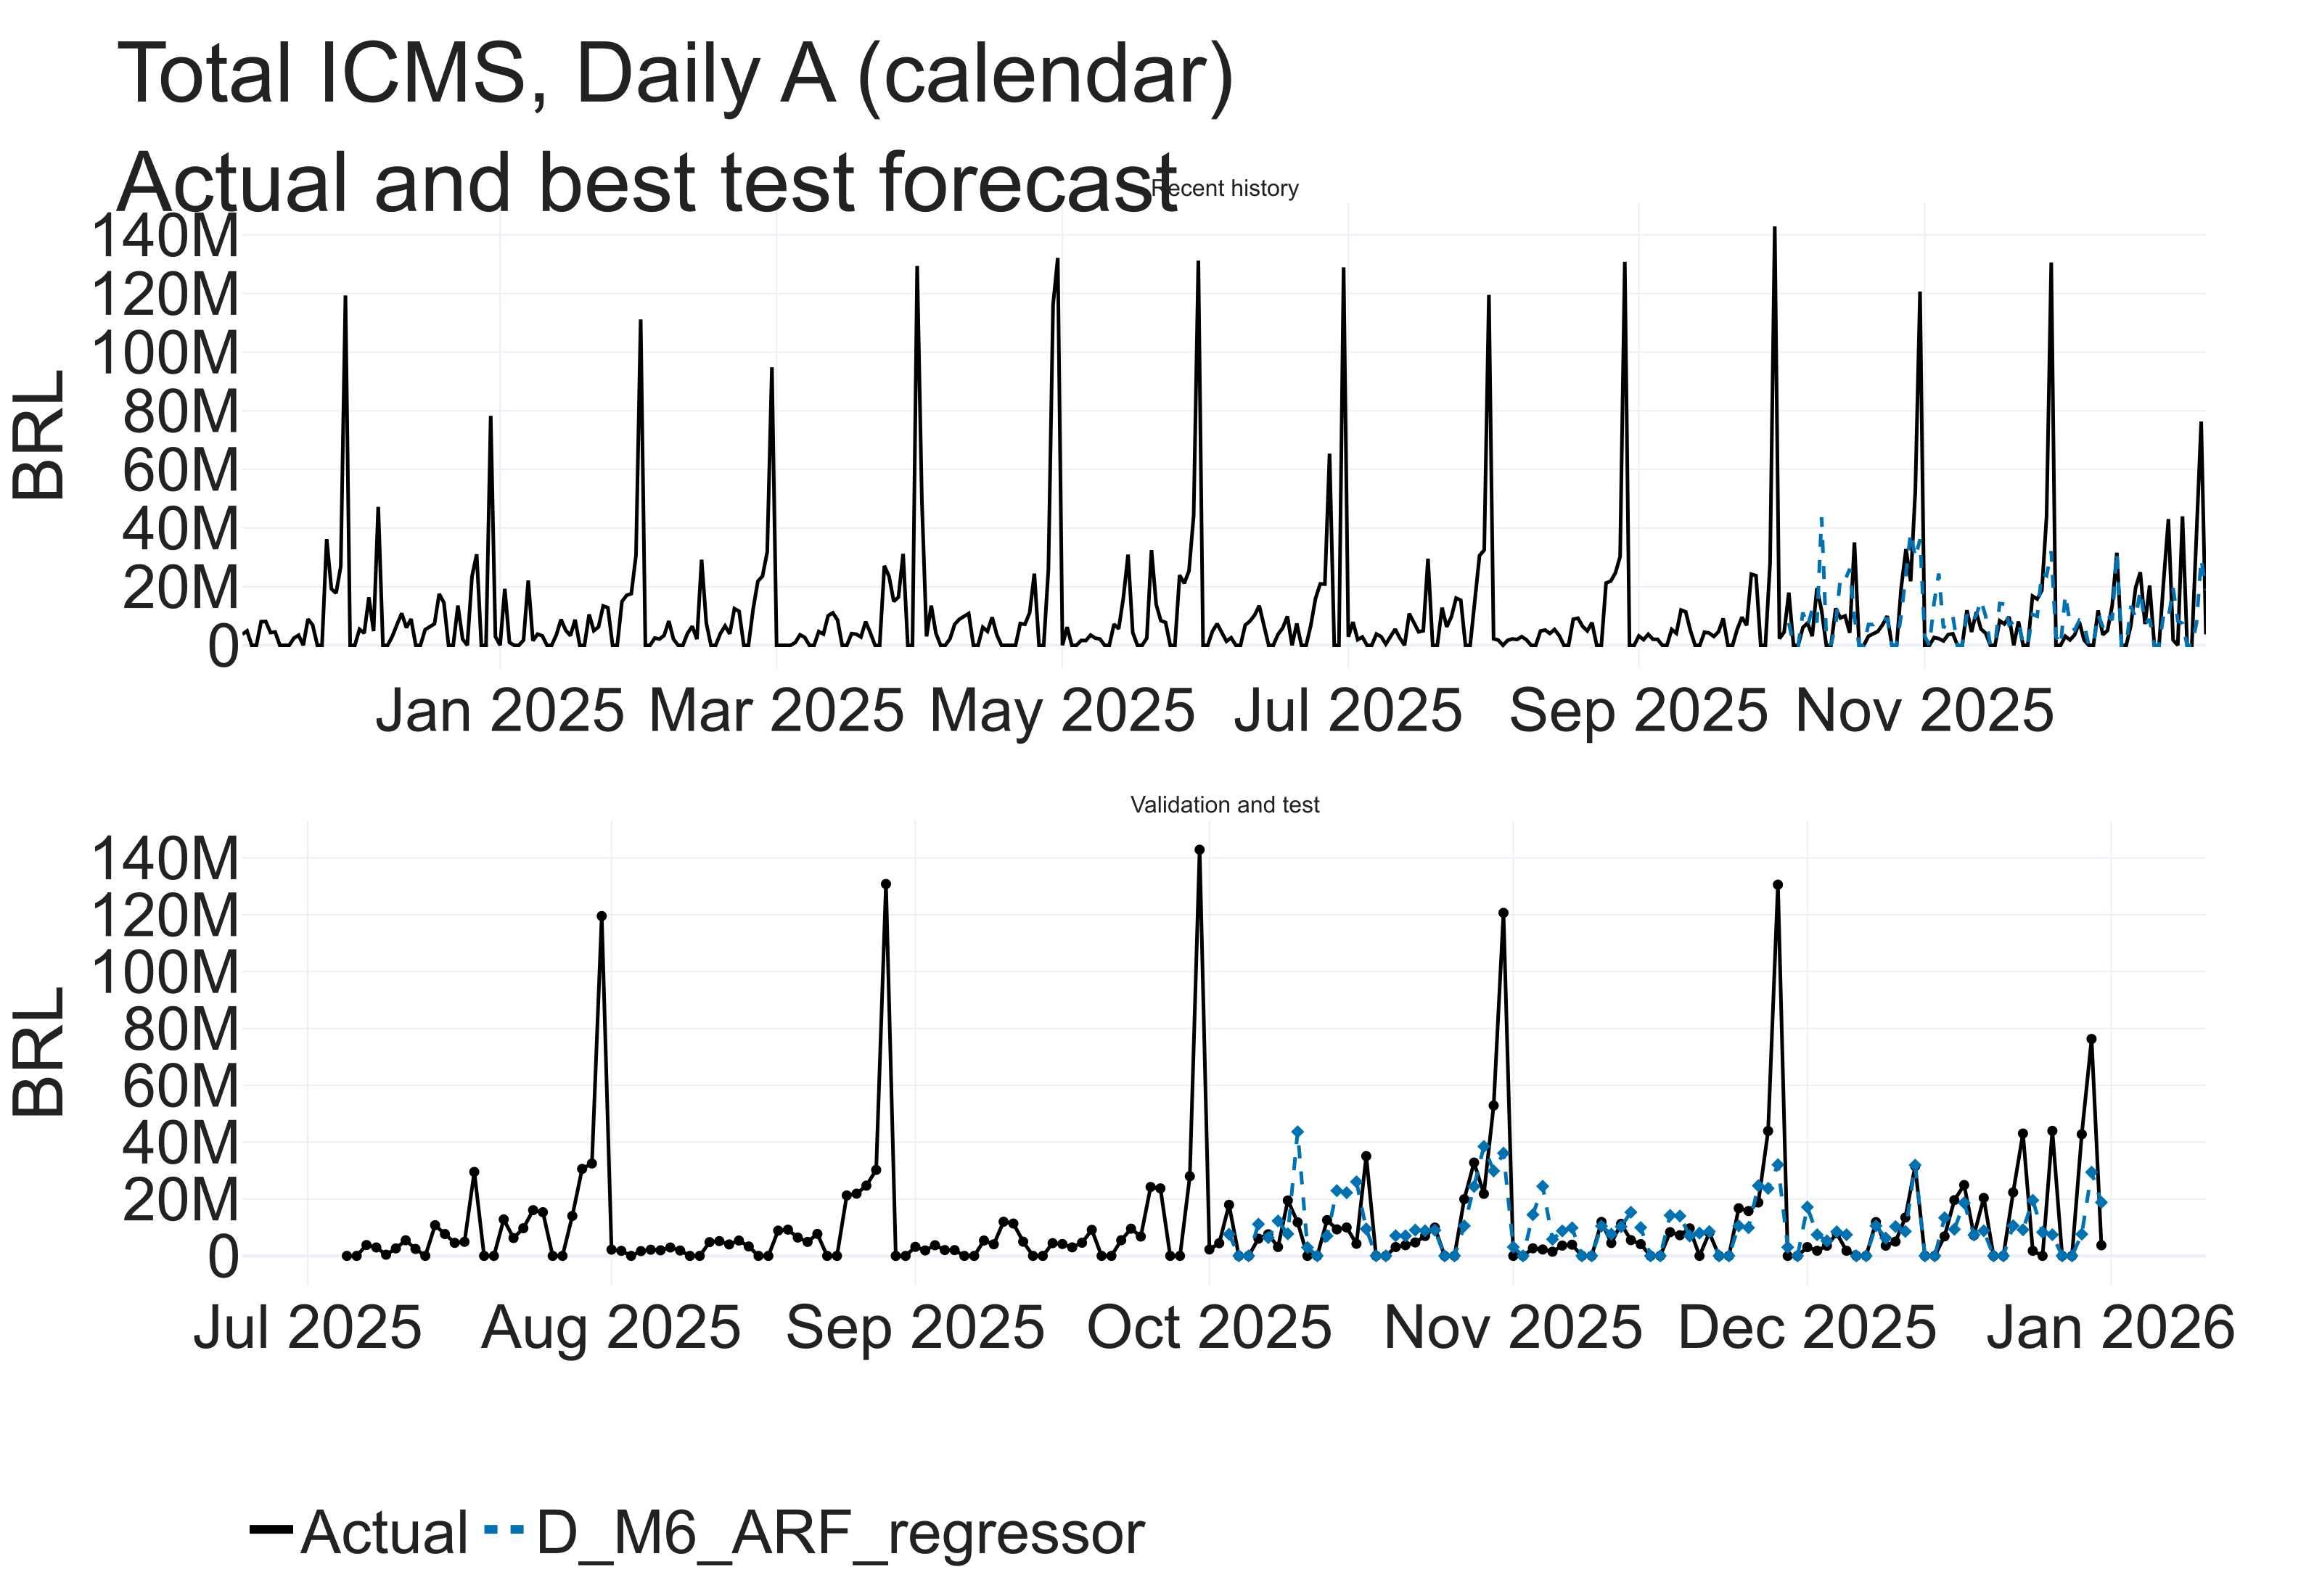
\includegraphics[width=\linewidth]{figures/segment/total_daily_forecast.png}
  \caption{Total, daily A. Blue dashed: M6 forest.}
\end{figure}
\begin{figure}[H]
  \centering
  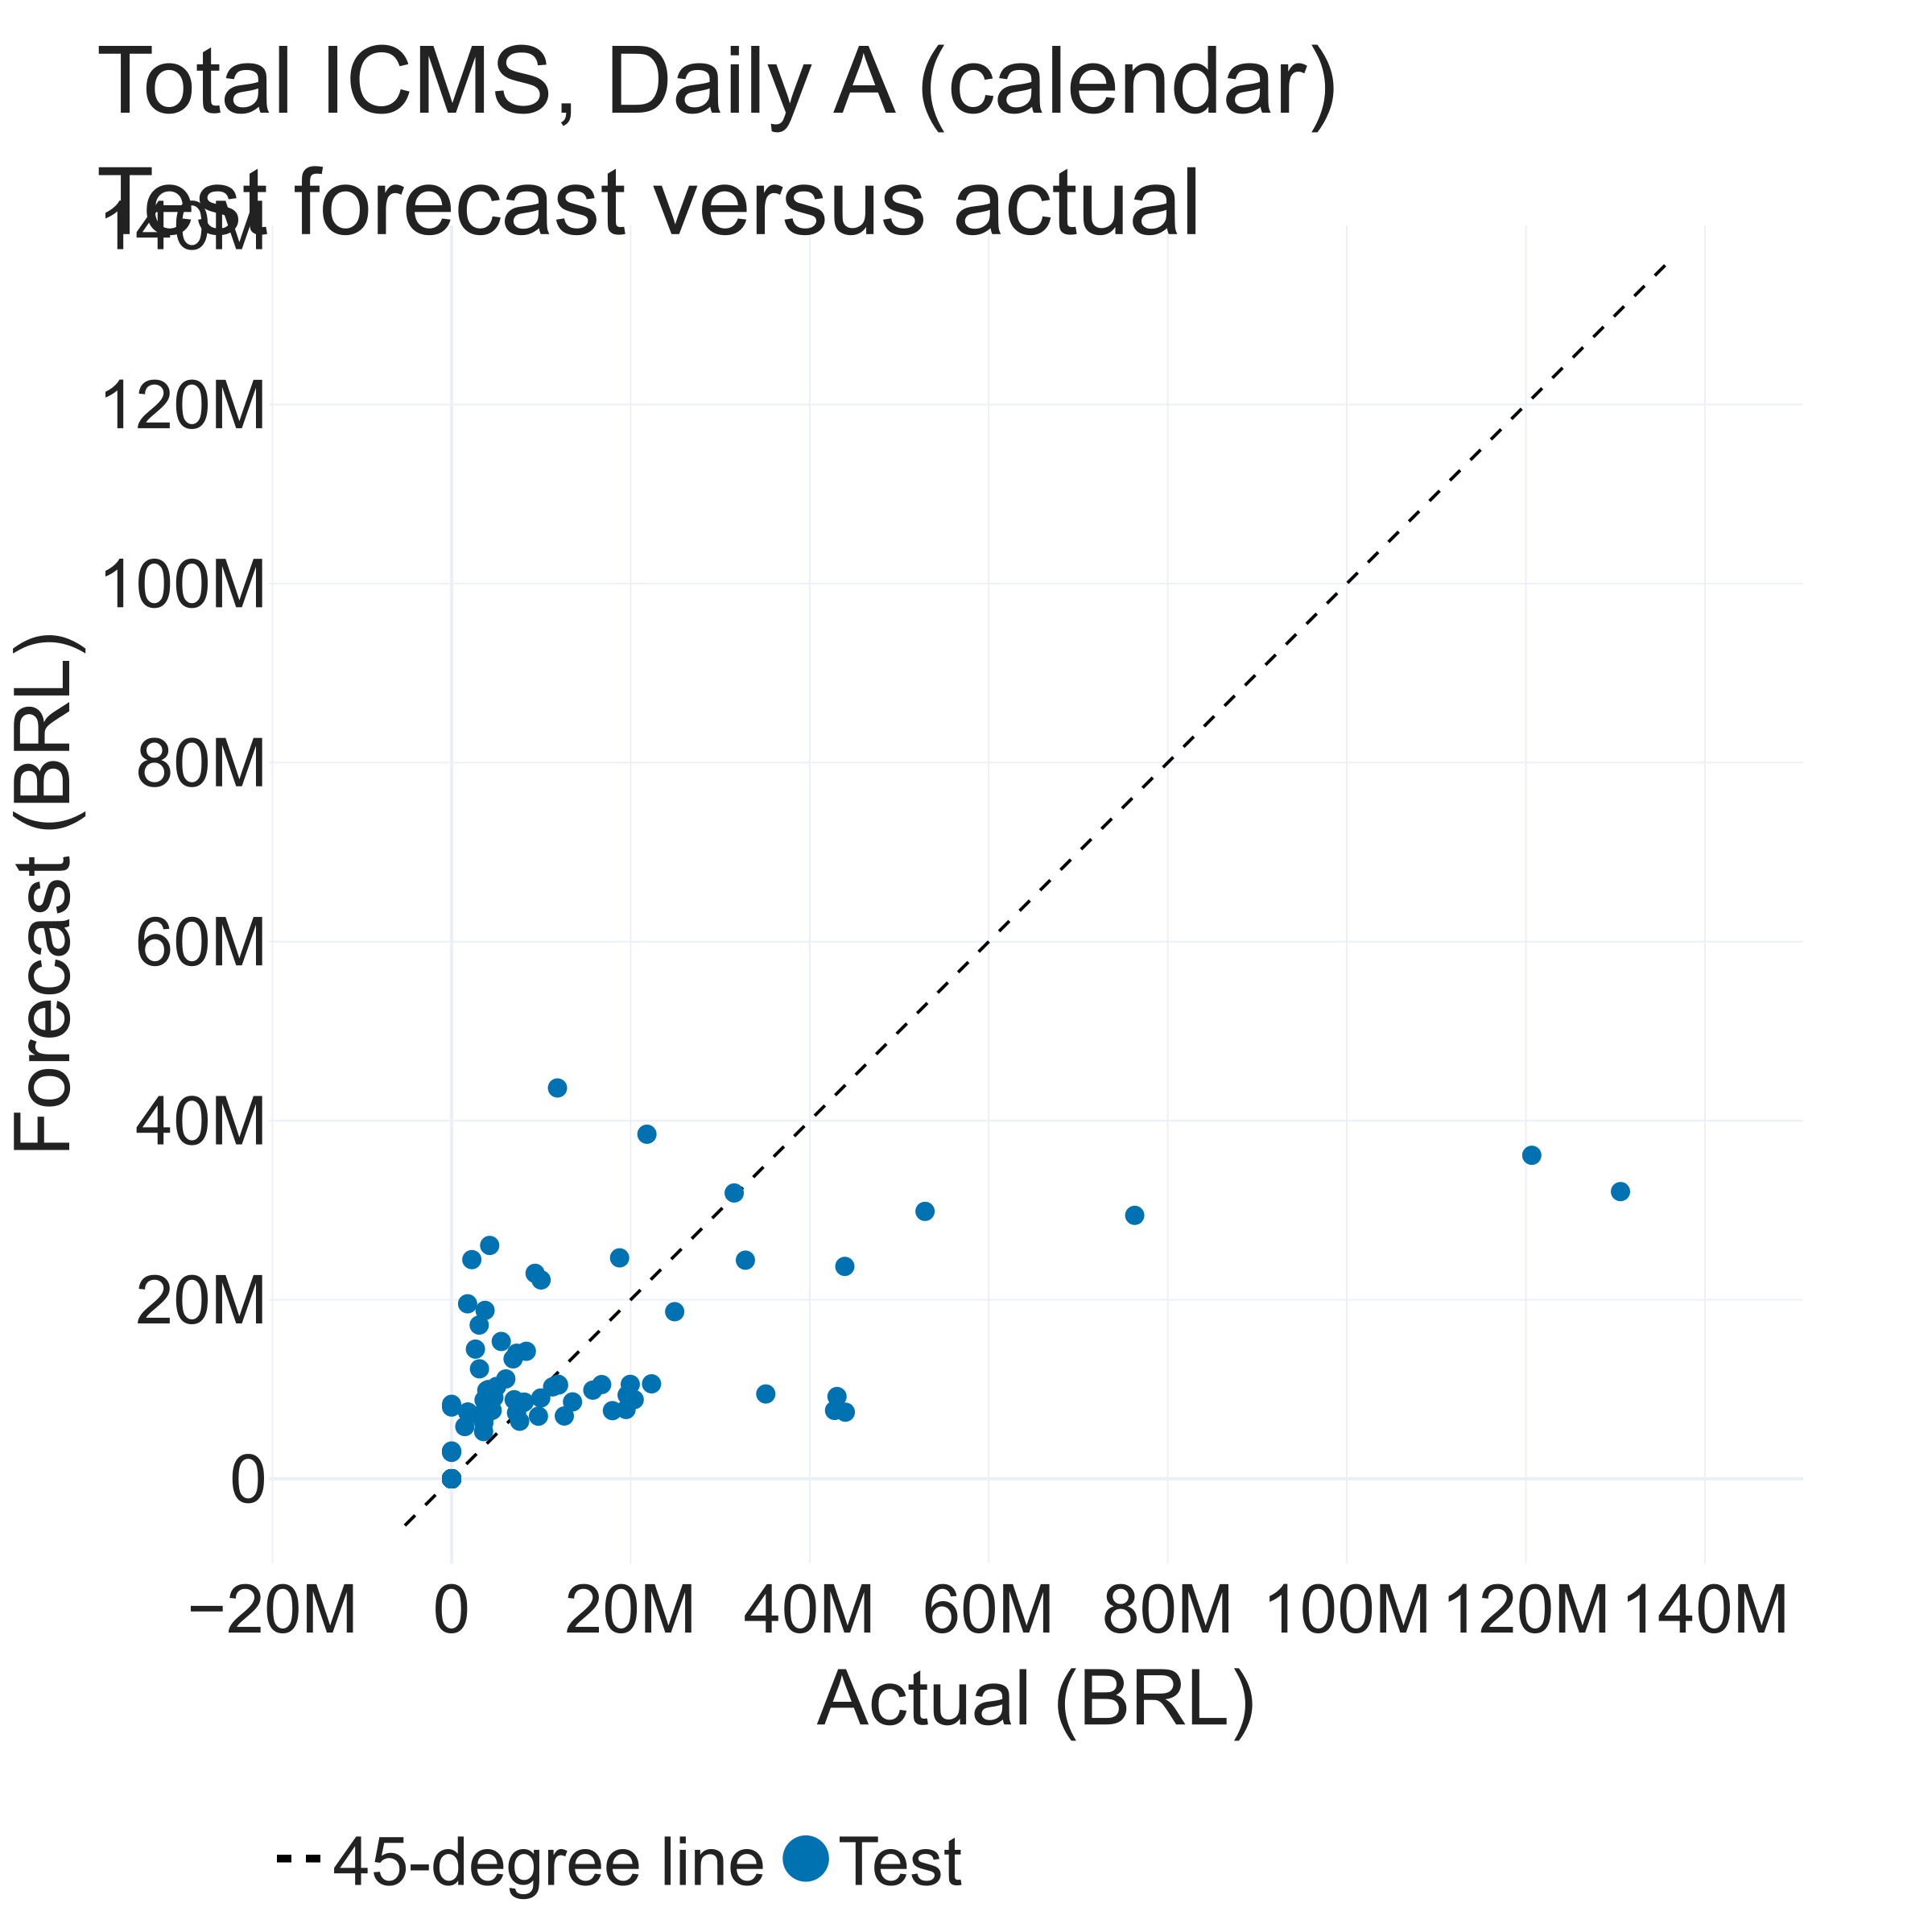
\includegraphics[width=0.62\linewidth]{figures/segment/total_daily_scatter.png}
  \caption{Total, daily A test scatter.}
\end{figure}
\begin{figure}[H]
  \centering
  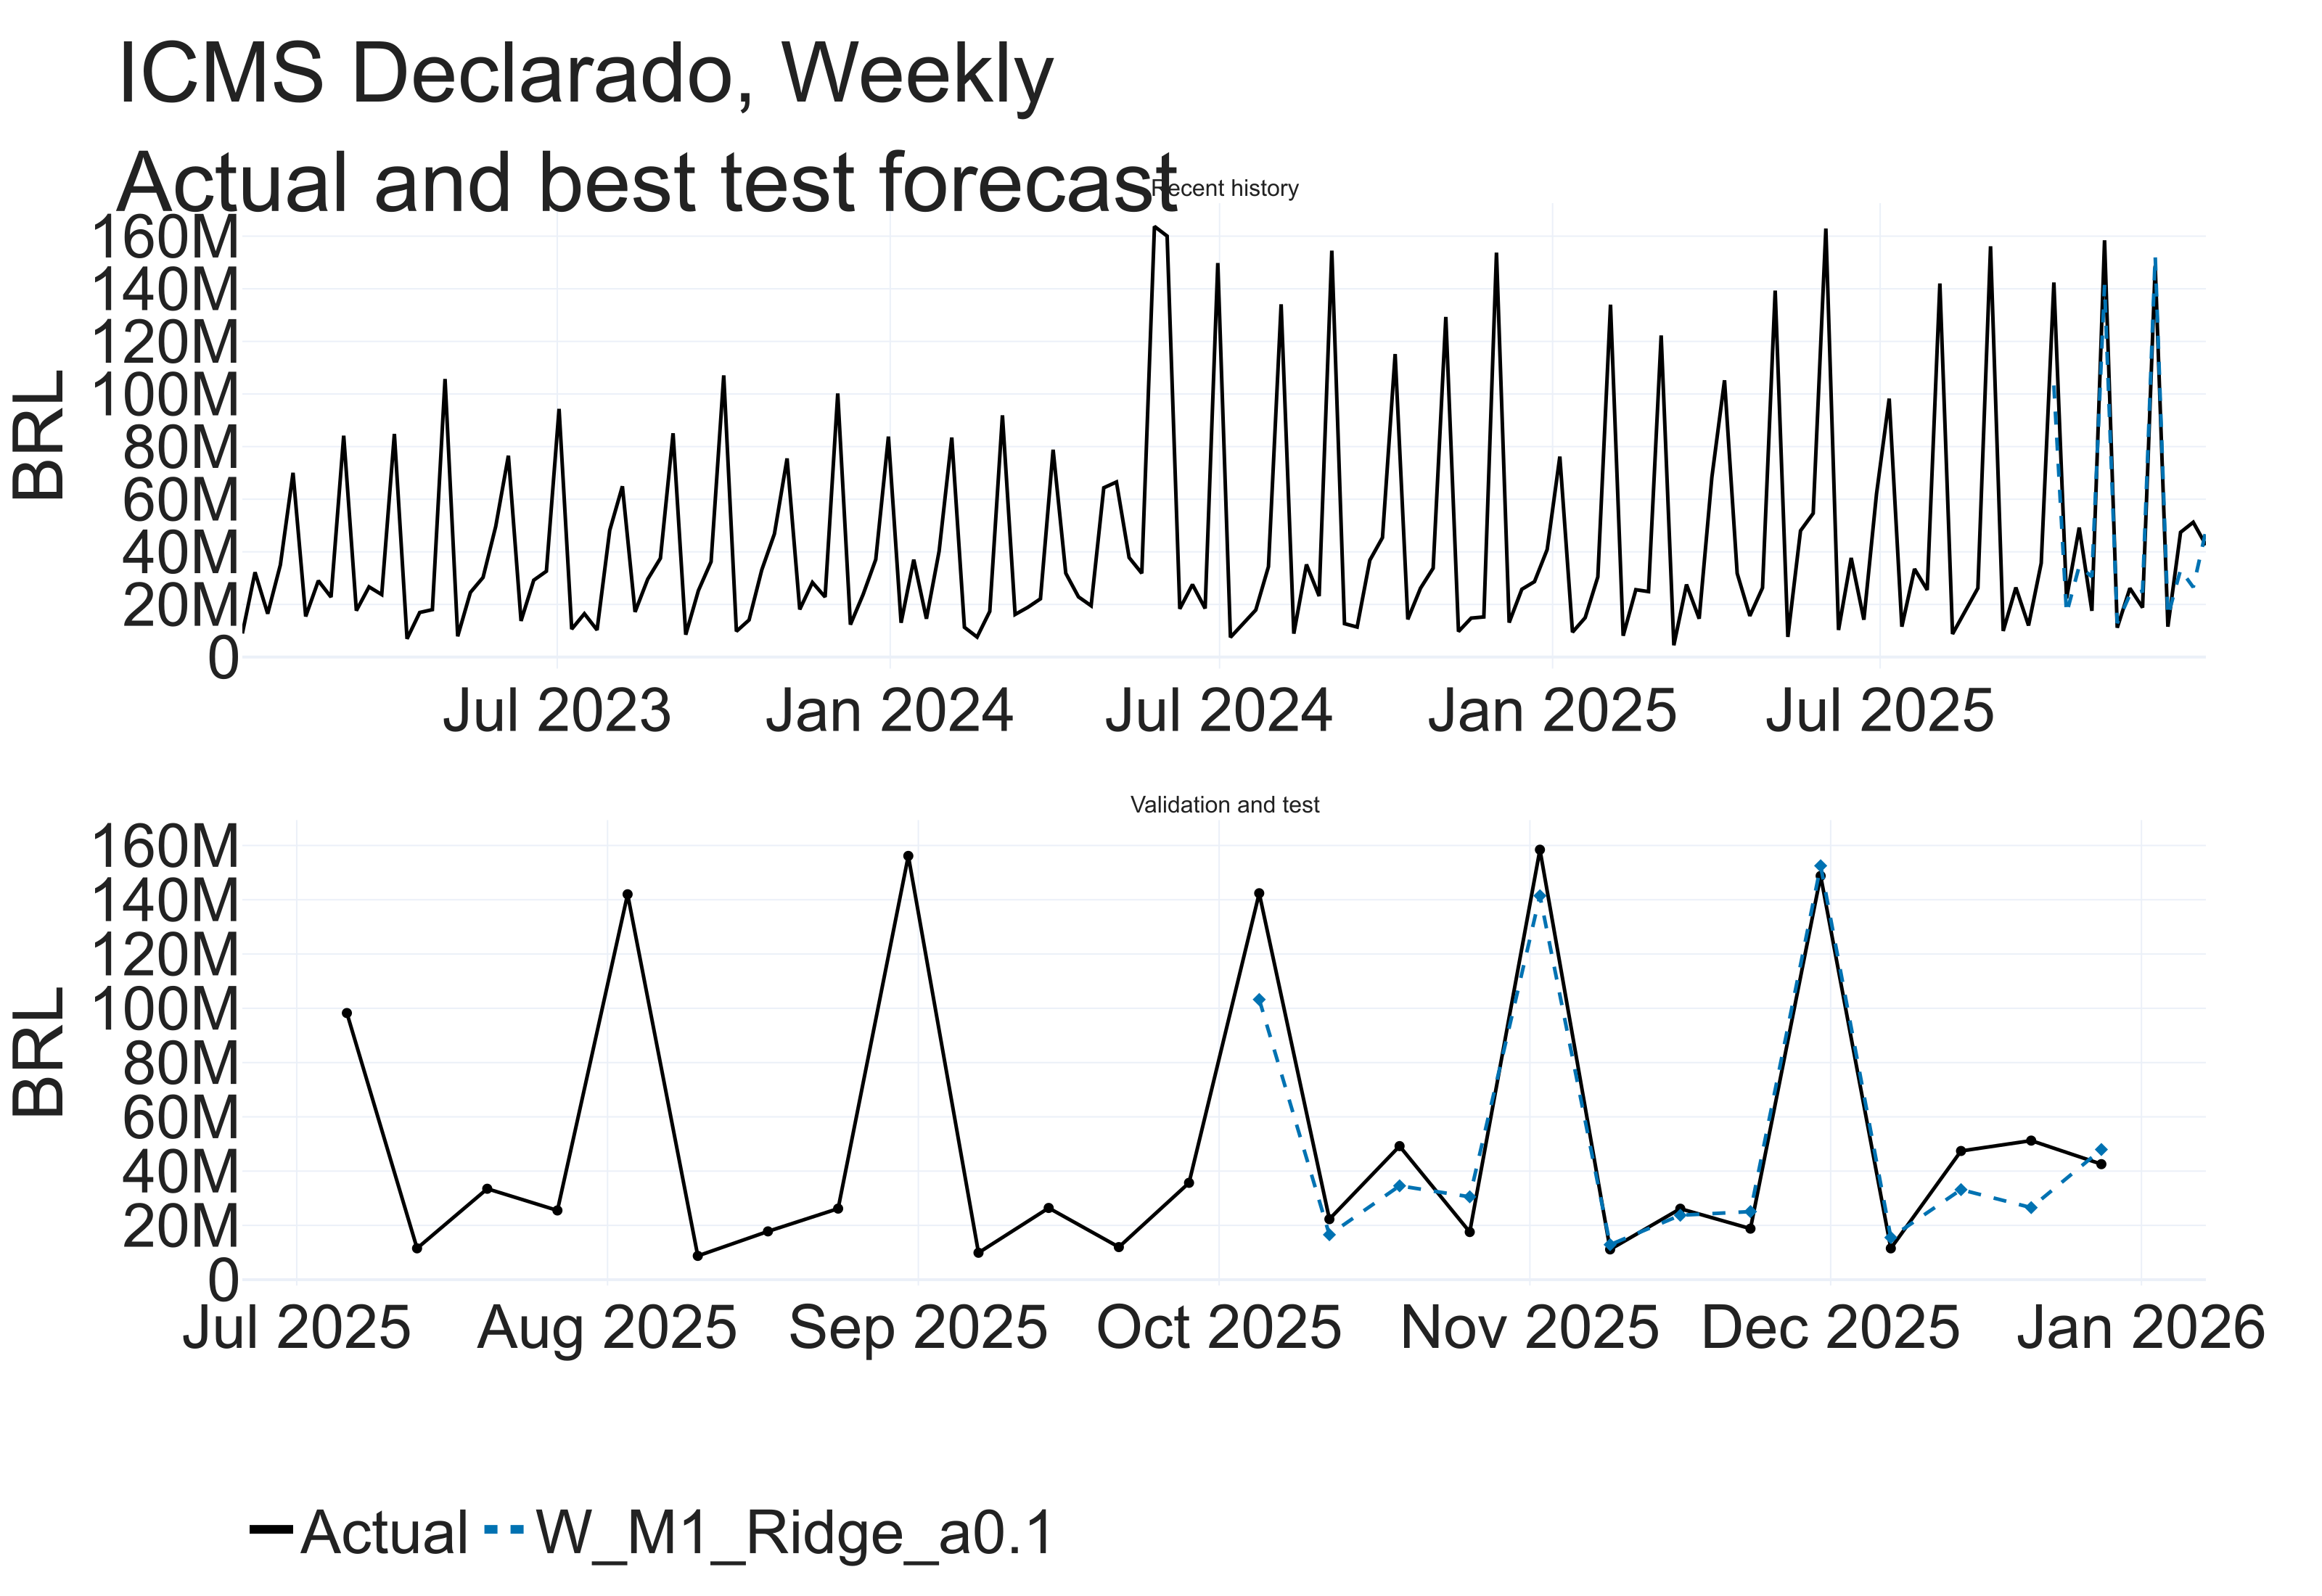
\includegraphics[width=\linewidth]{figures/segment/declarado_weekly_forecast.png}
  \caption{Declarado, weekly. Blue dashed: M1 ridge.}
\end{figure}
\begin{figure}[H]
  \centering
  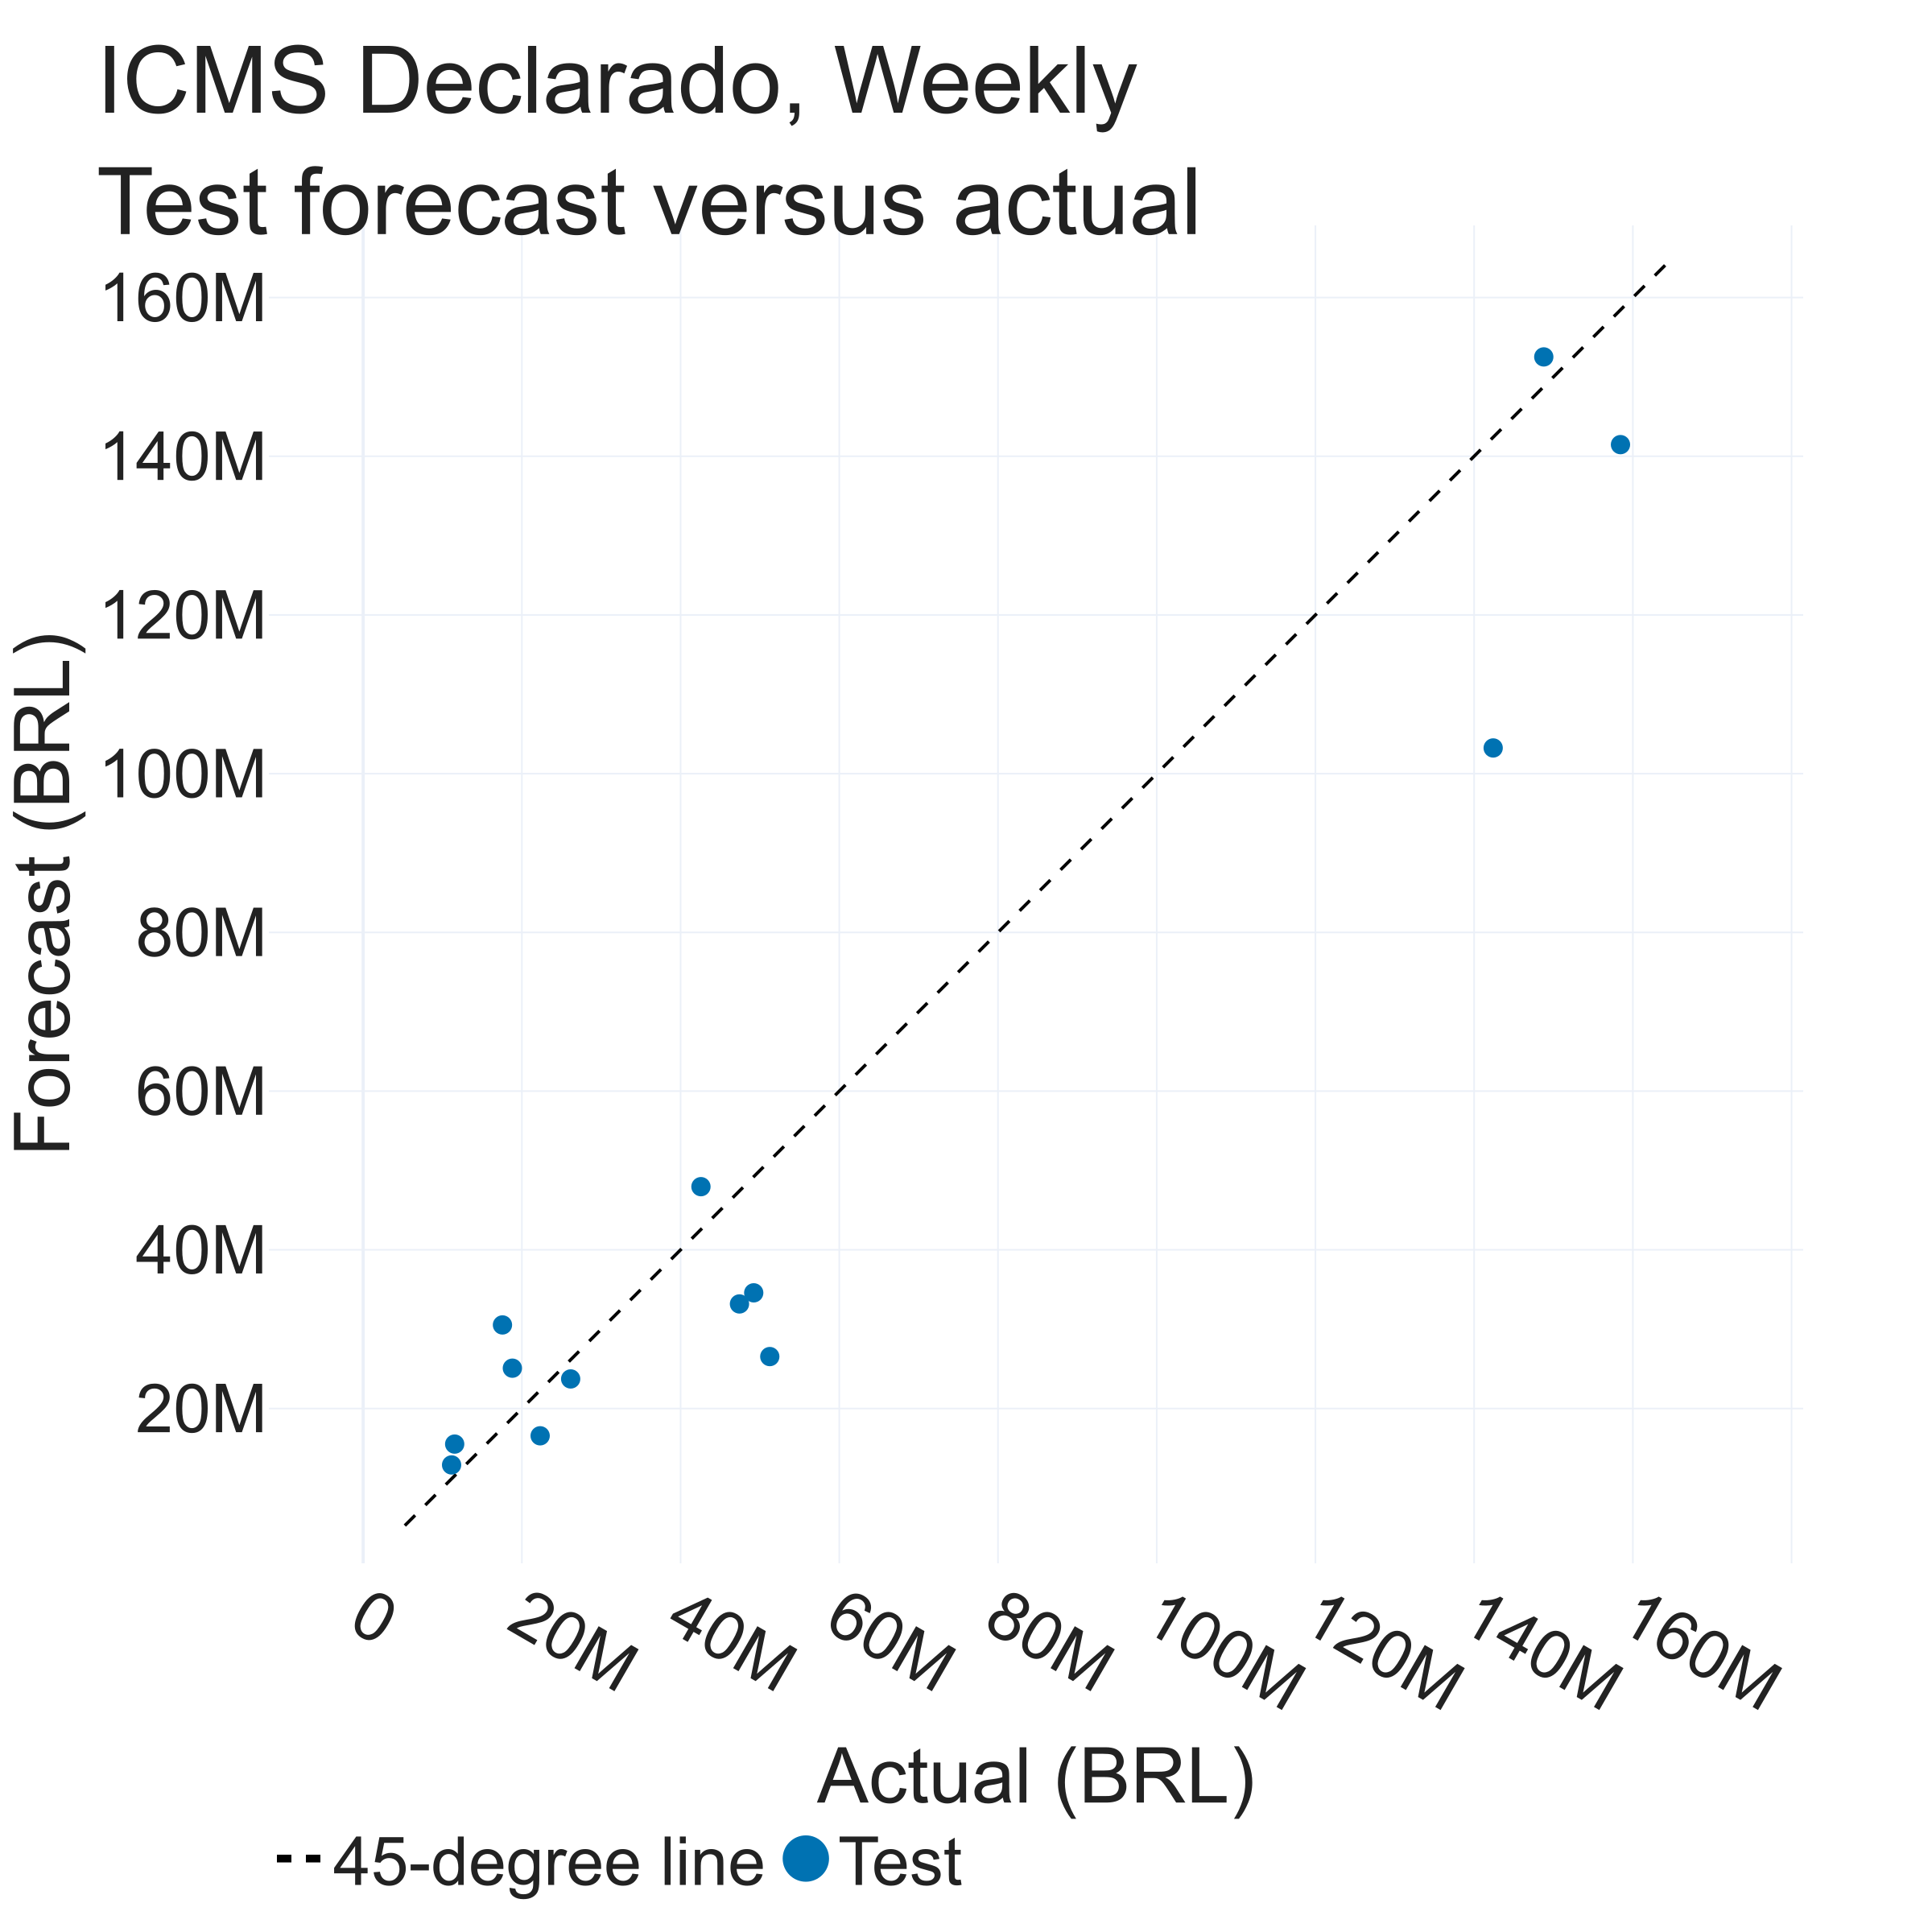
\includegraphics[width=0.62\linewidth]{figures/segment/declarado_weekly_scatter.png}
  \caption{Declarado, weekly test scatter.}
\end{figure}
\begin{figure}[H]
  \centering
  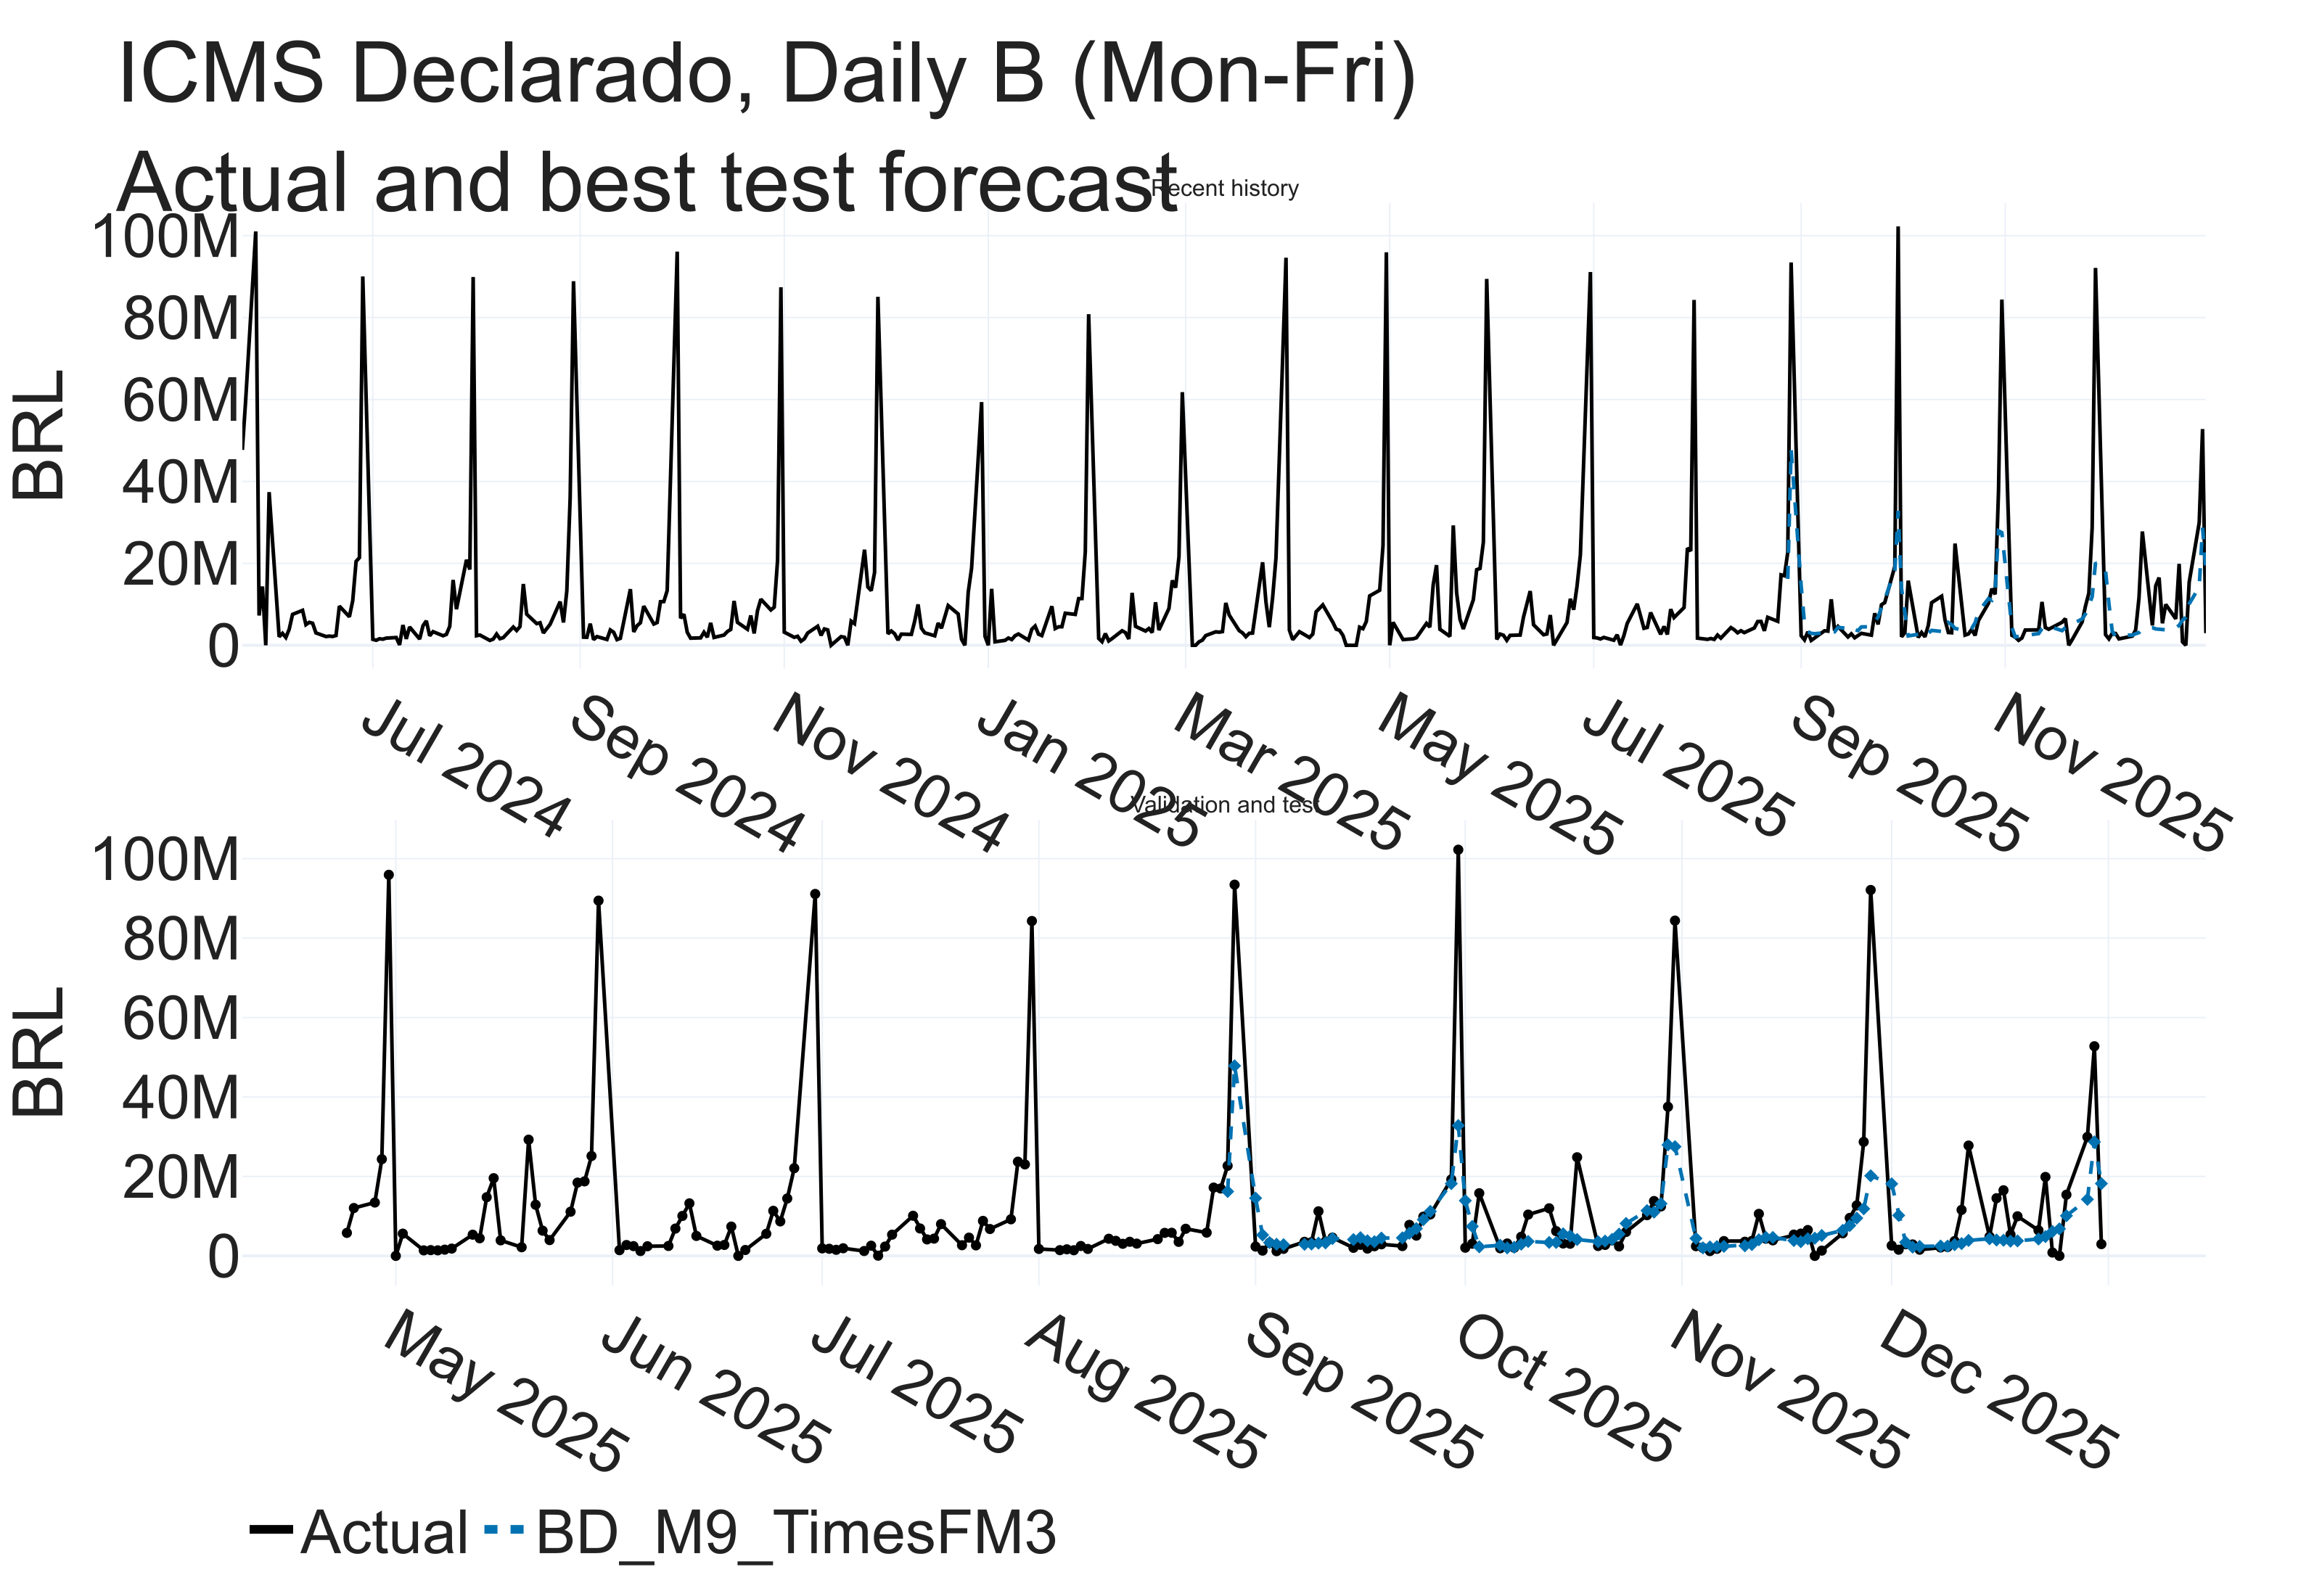
\includegraphics[width=\linewidth]{figures/segment/declarado_business_daily_forecast.png}
  \caption{Declarado, daily B. Blue dashed: M9 TimesFM.}
\end{figure}
\begin{figure}[H]
  \centering
  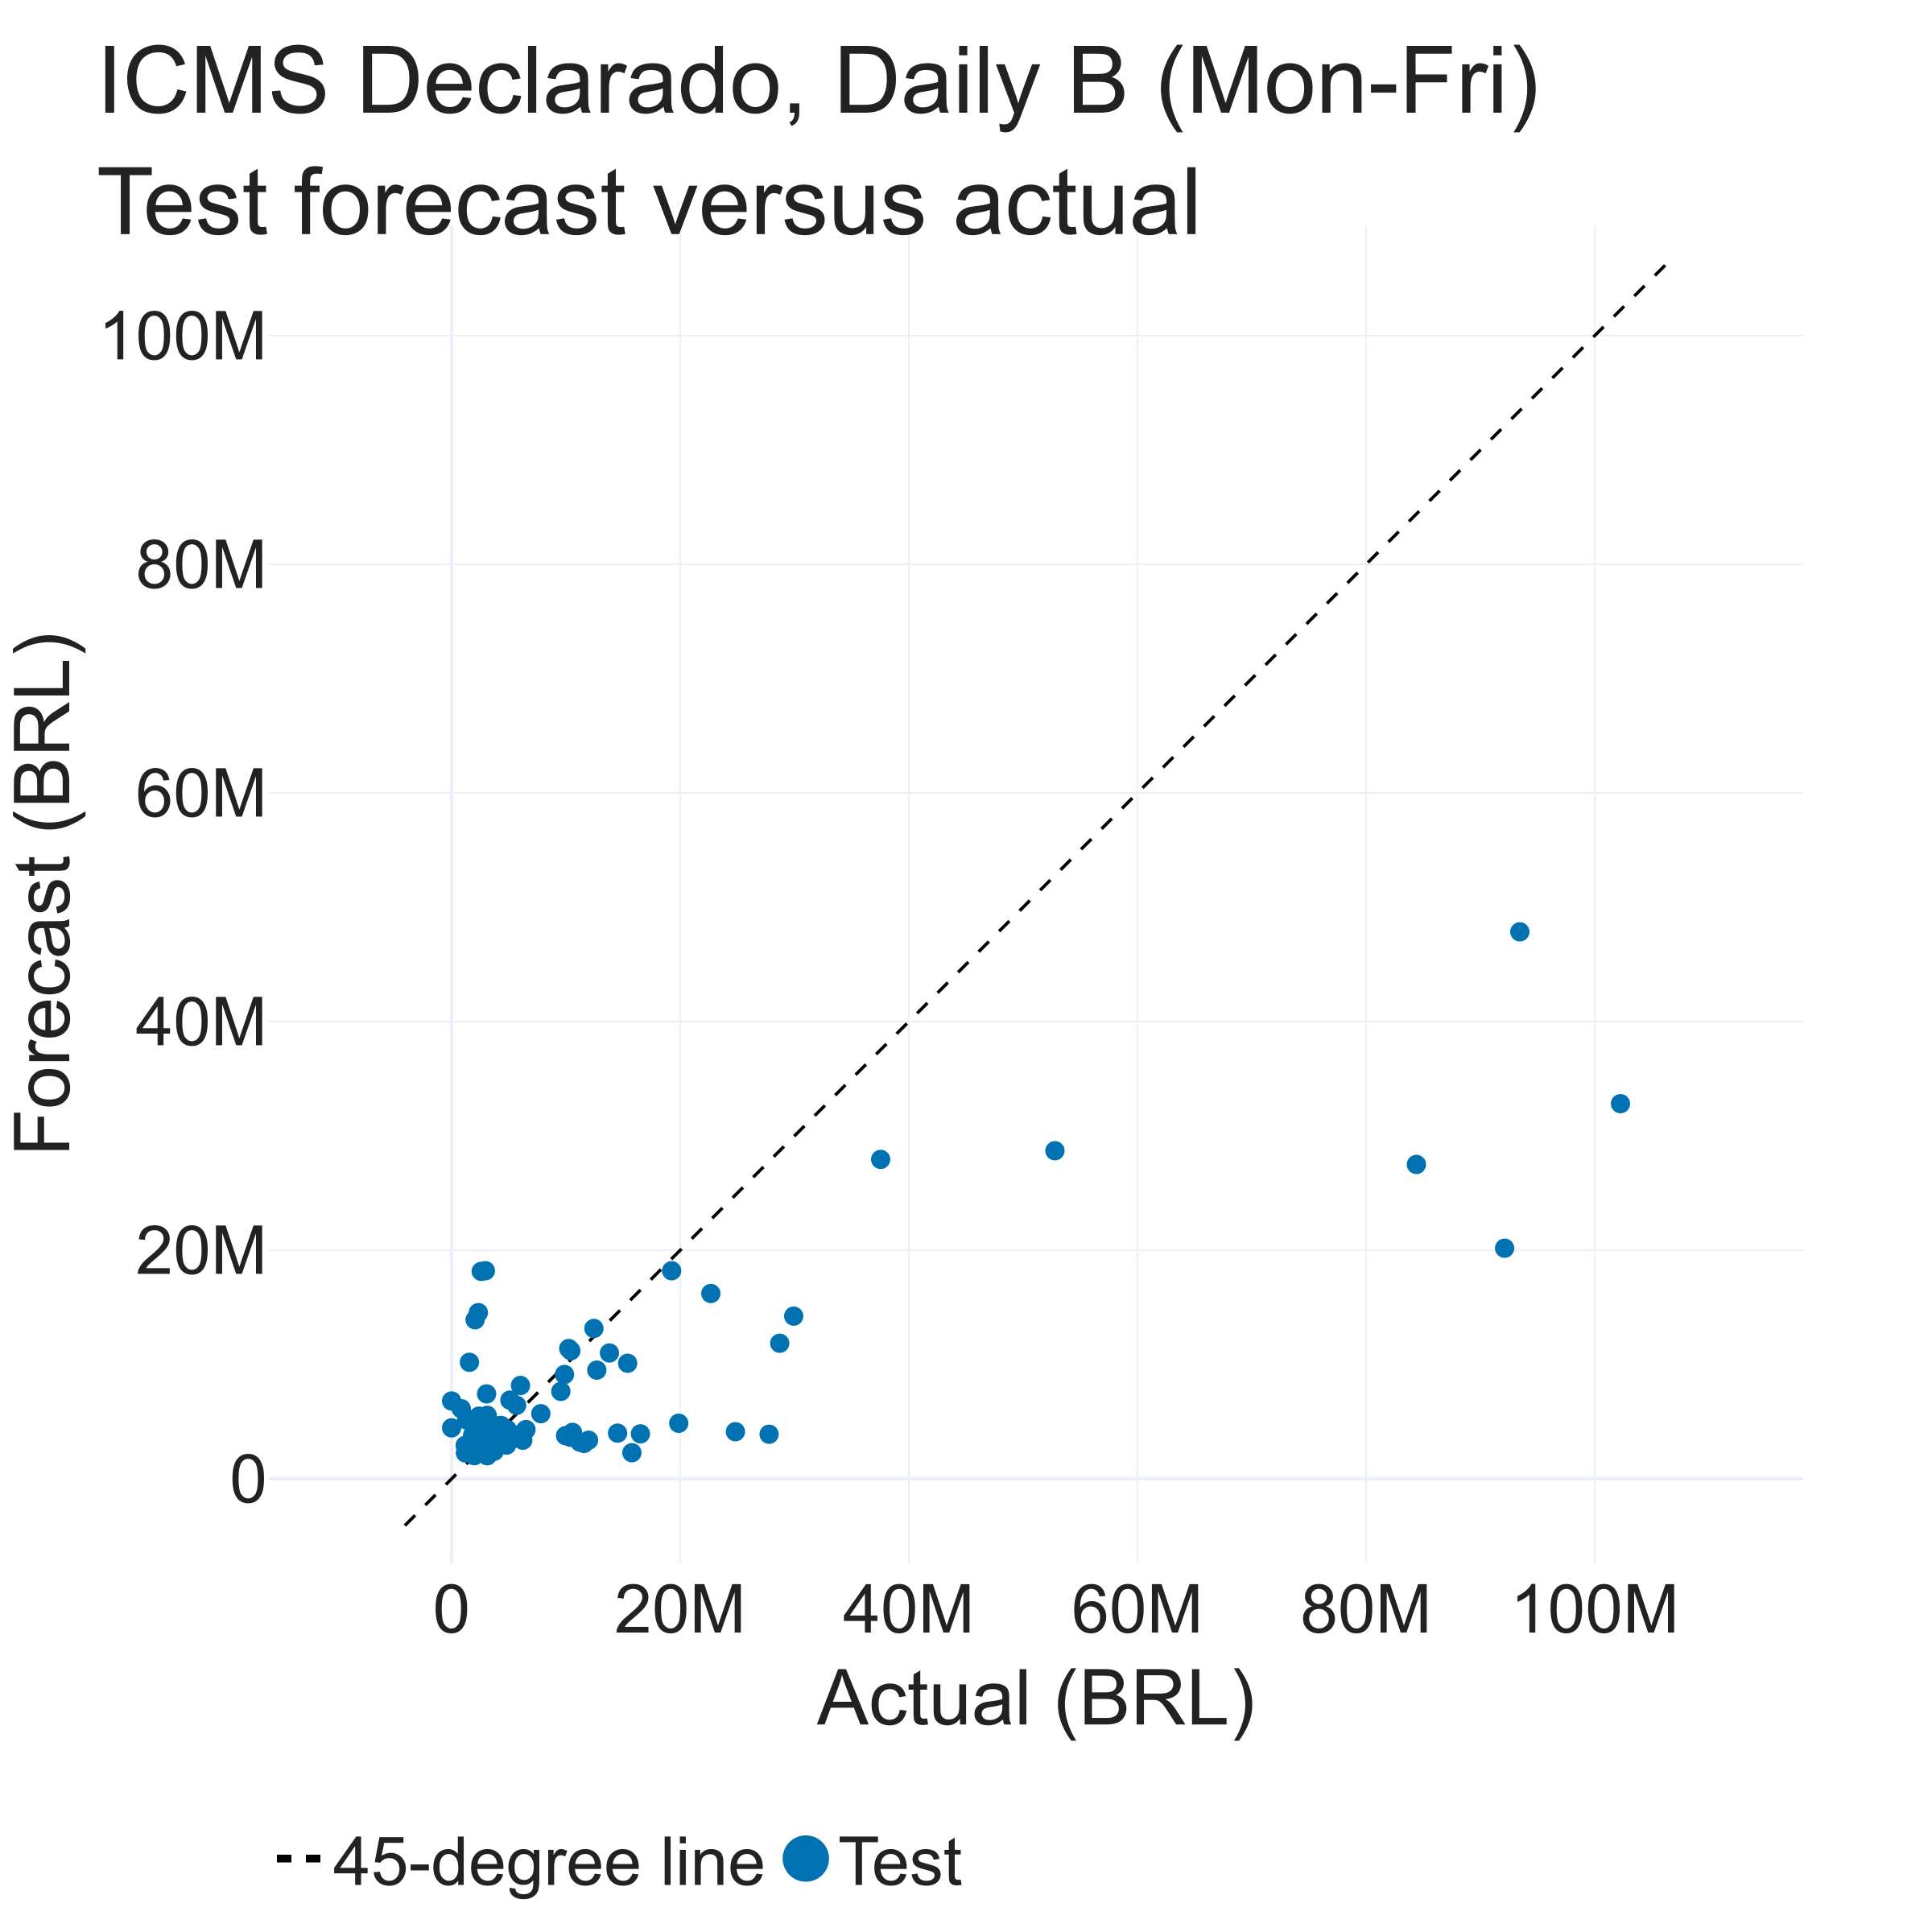
\includegraphics[width=0.62\linewidth]{figures/segment/declarado_business_daily_scatter.png}
  \caption{Declarado, daily B test scatter.}
\end{figure}
\begin{figure}[H]
  \centering
  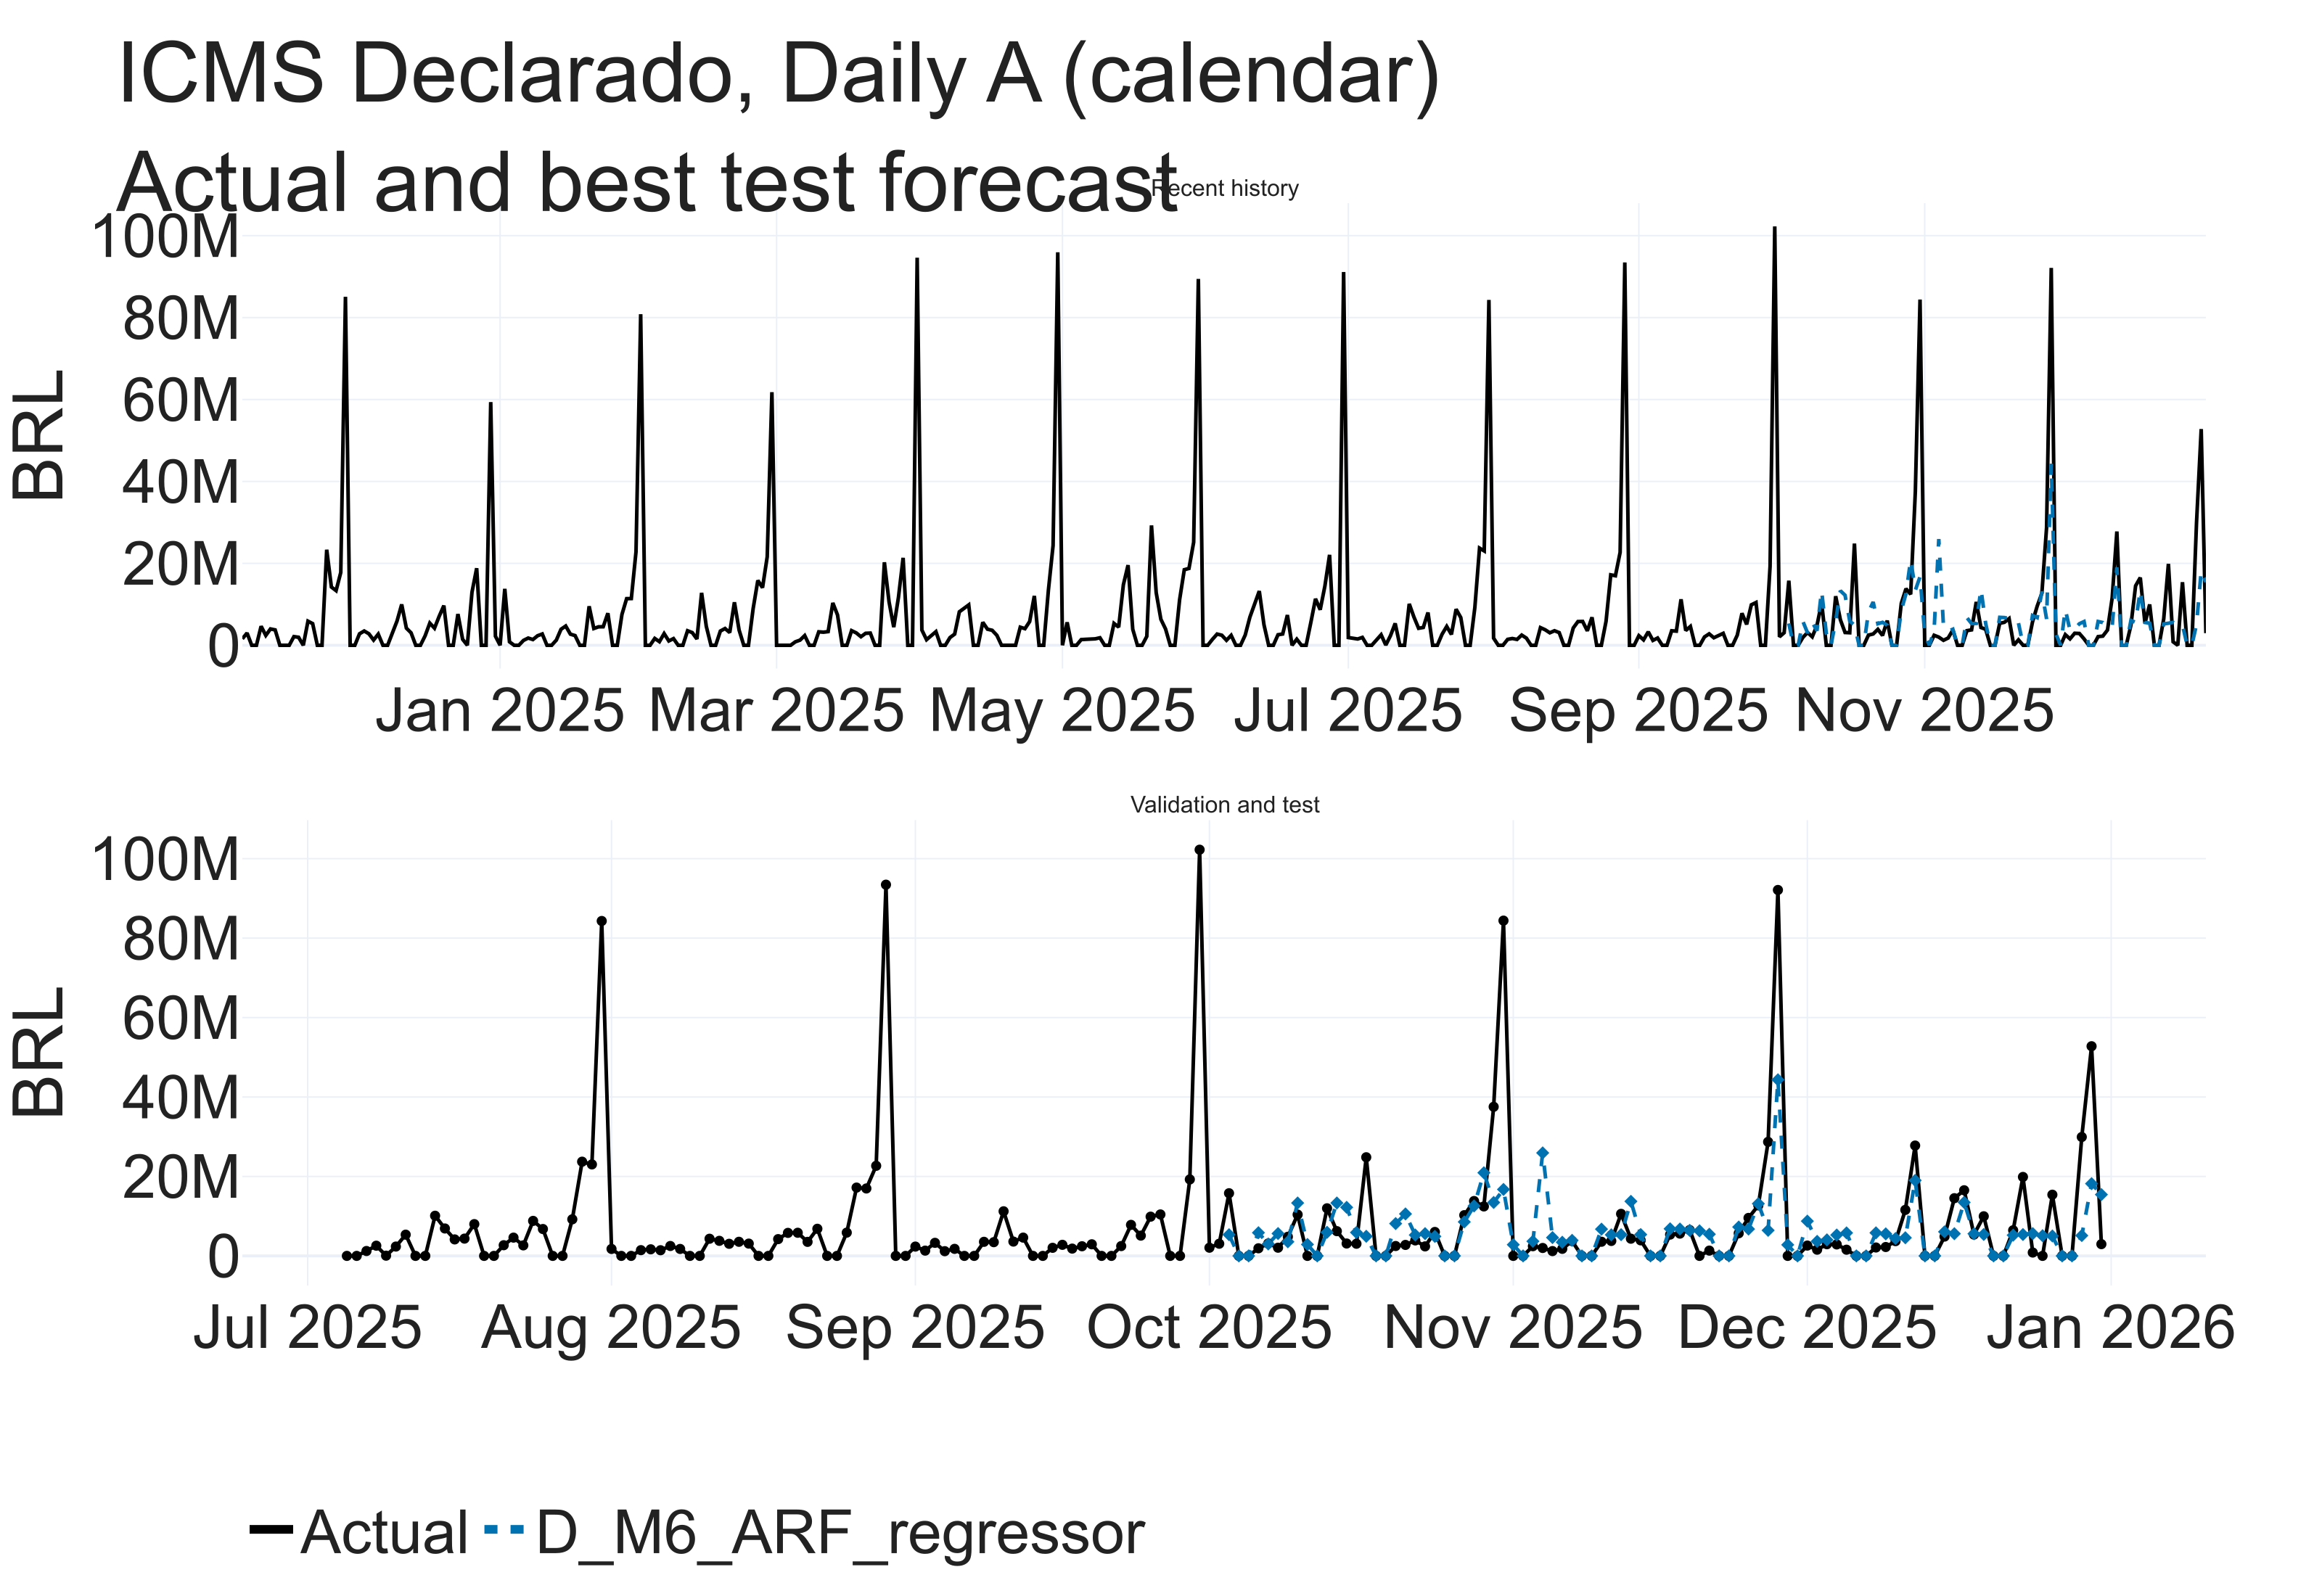
\includegraphics[width=\linewidth]{figures/segment/declarado_daily_forecast.png}
  \caption{Declarado, daily A. Blue dashed: M6 forest.}
\end{figure}
\begin{figure}[H]
  \centering
  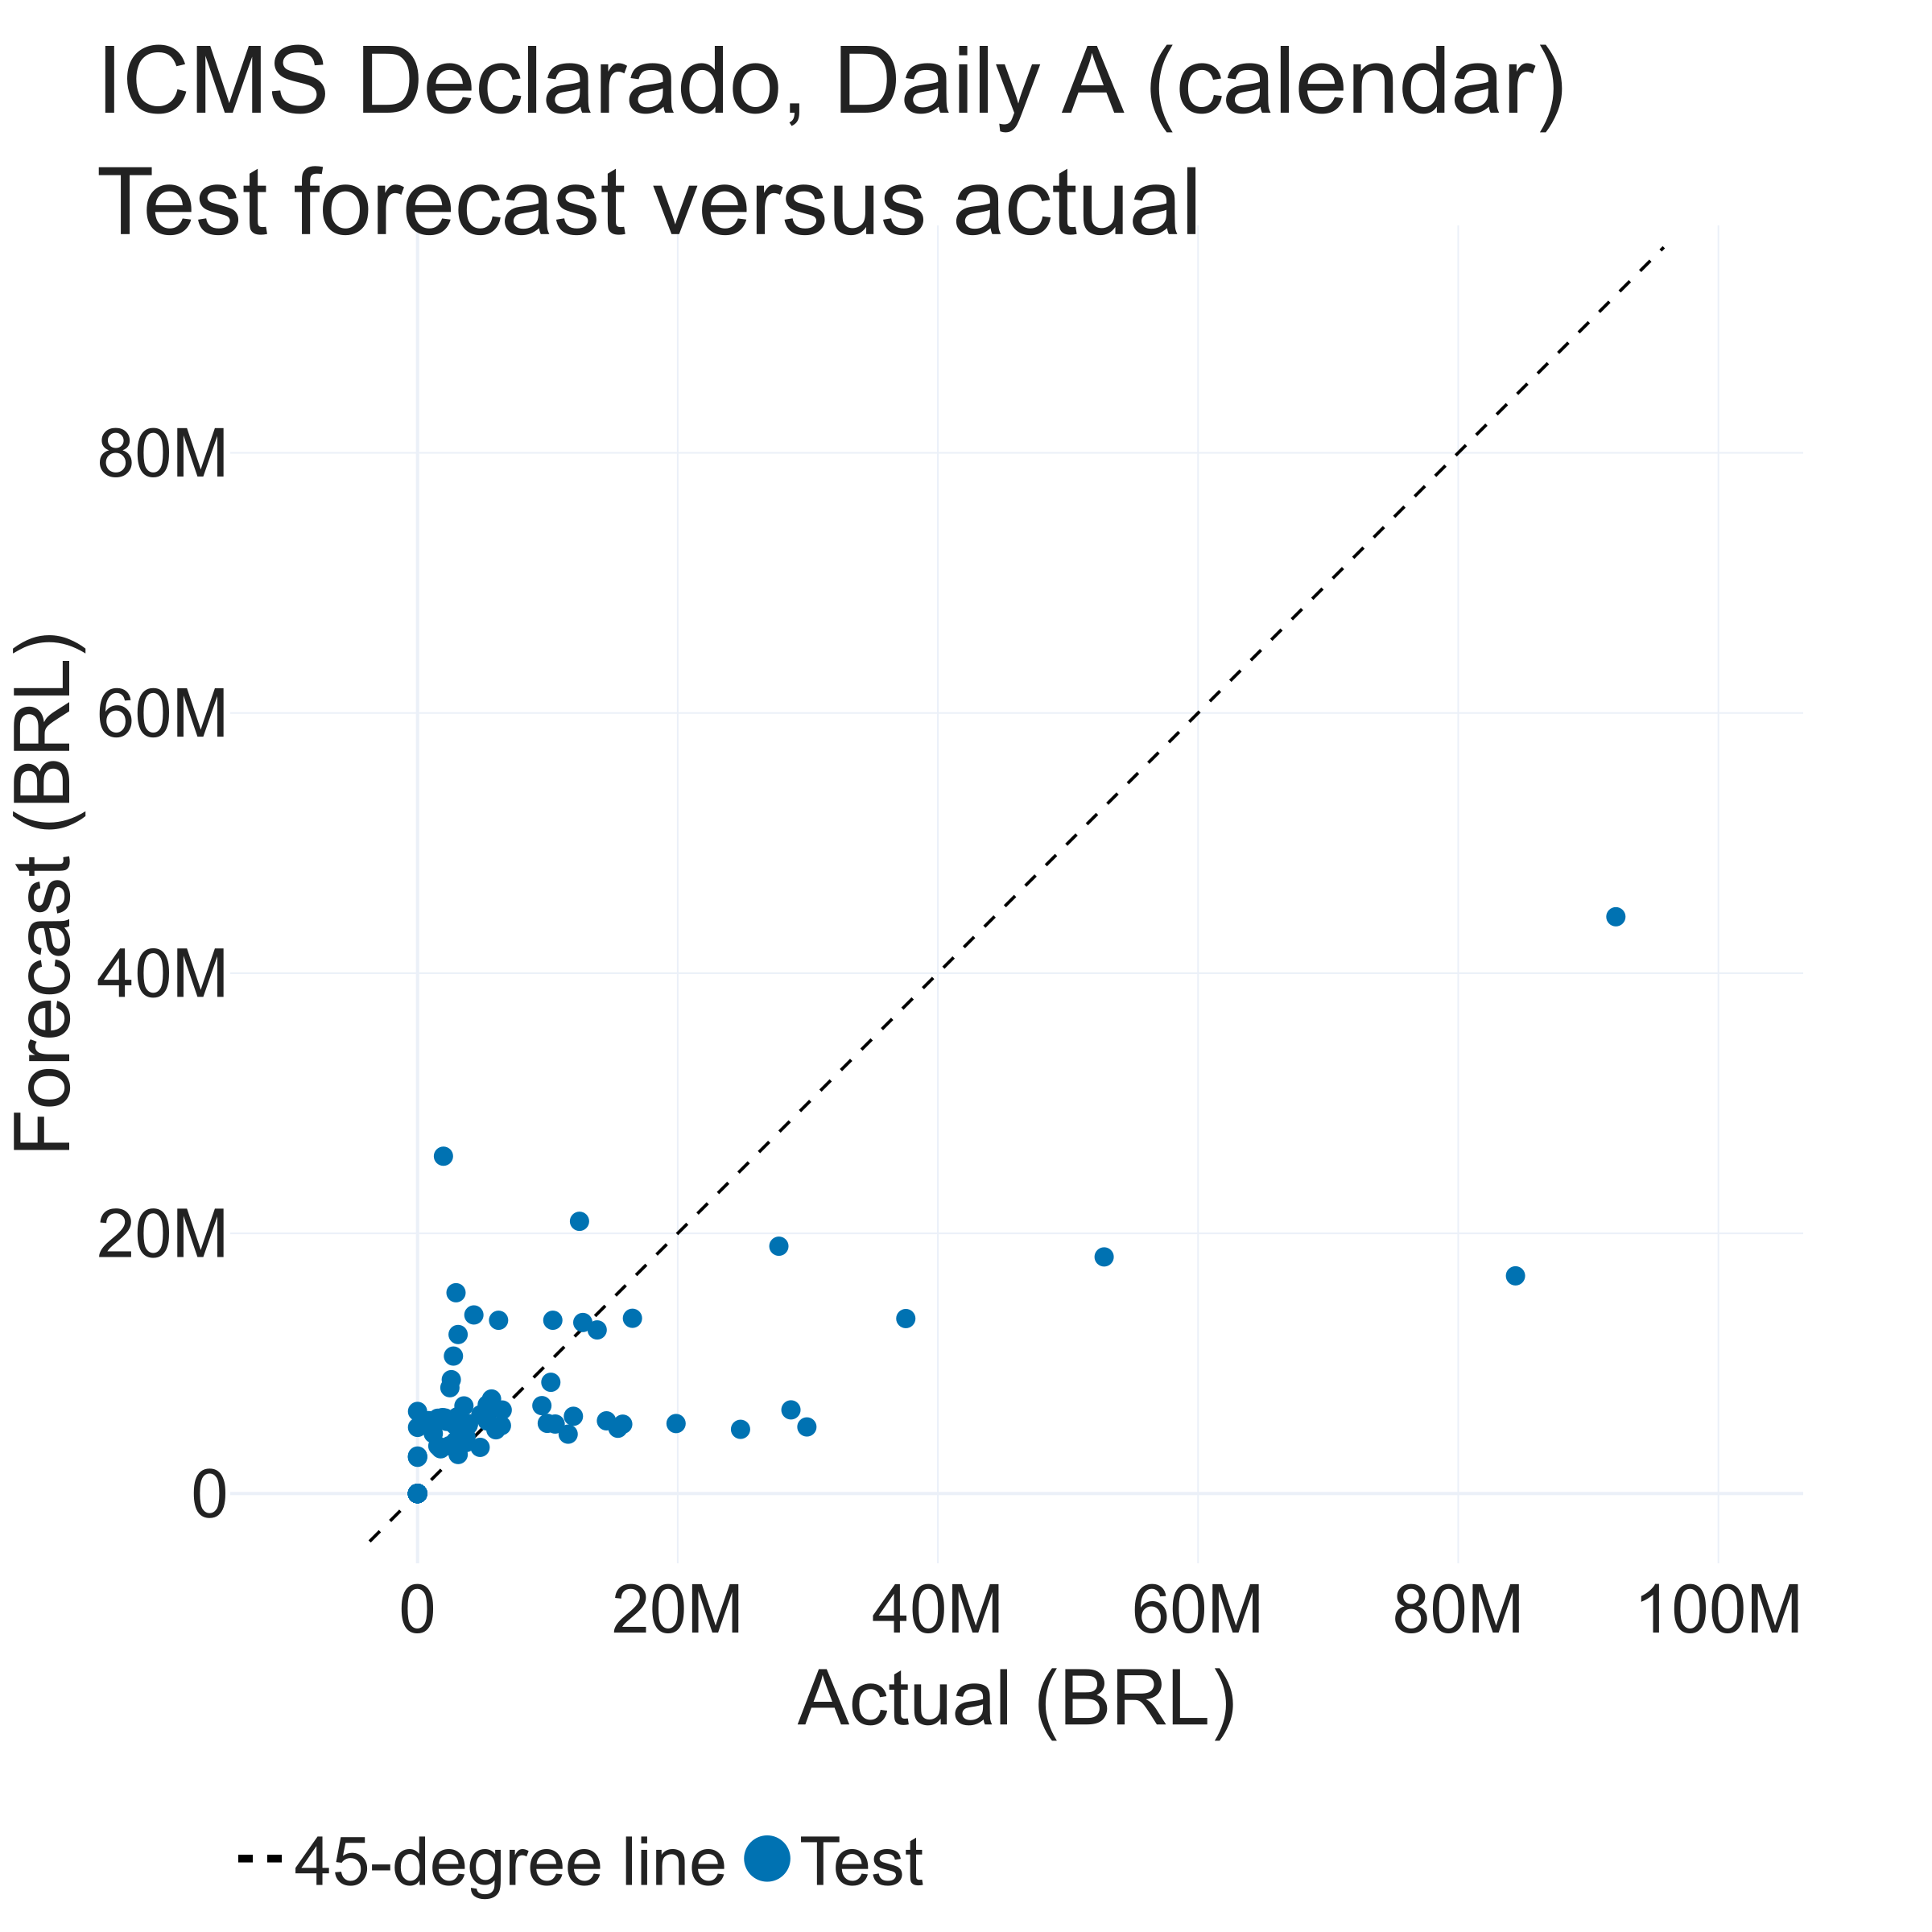
\includegraphics[width=0.62\linewidth]{figures/segment/declarado_daily_scatter.png}
  \caption{Declarado, daily A test scatter.}
\end{figure}
\begin{figure}[H]
  \centering
  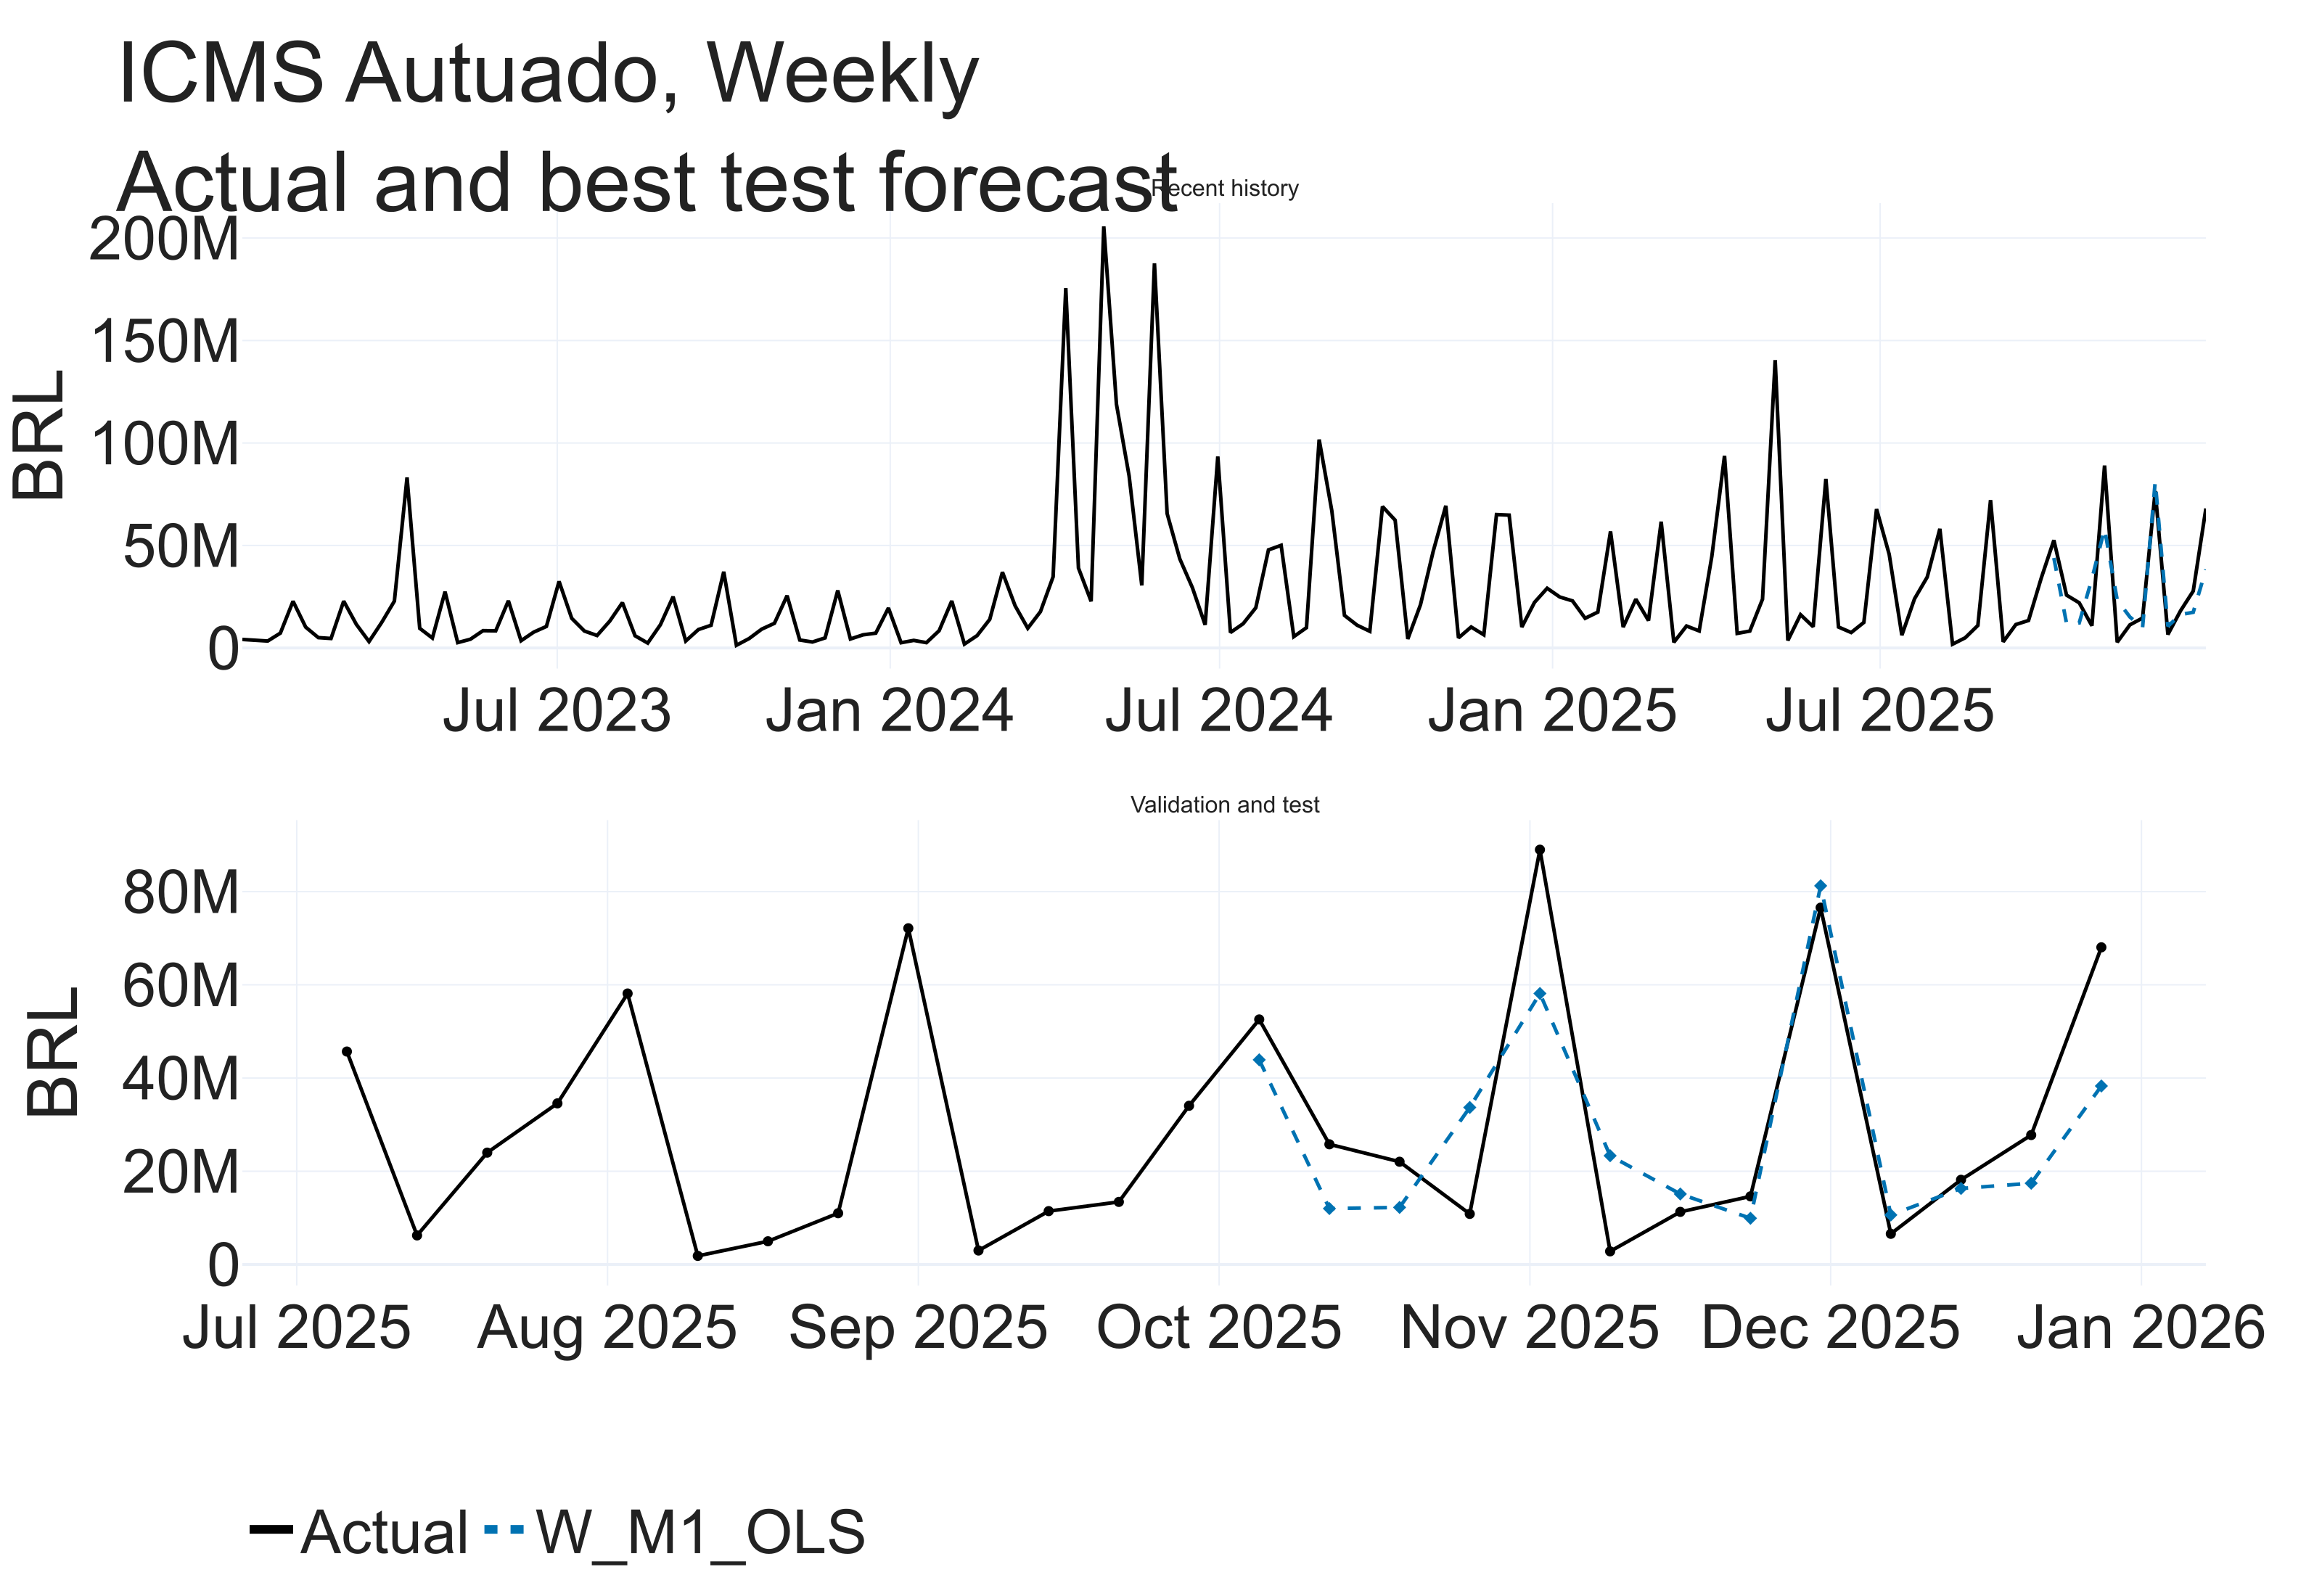
\includegraphics[width=\linewidth]{figures/segment/autuado_weekly_forecast.png}
  \caption{Autuado, weekly. Blue dashed: M1 least squares.}
\end{figure}
\begin{figure}[H]
  \centering
  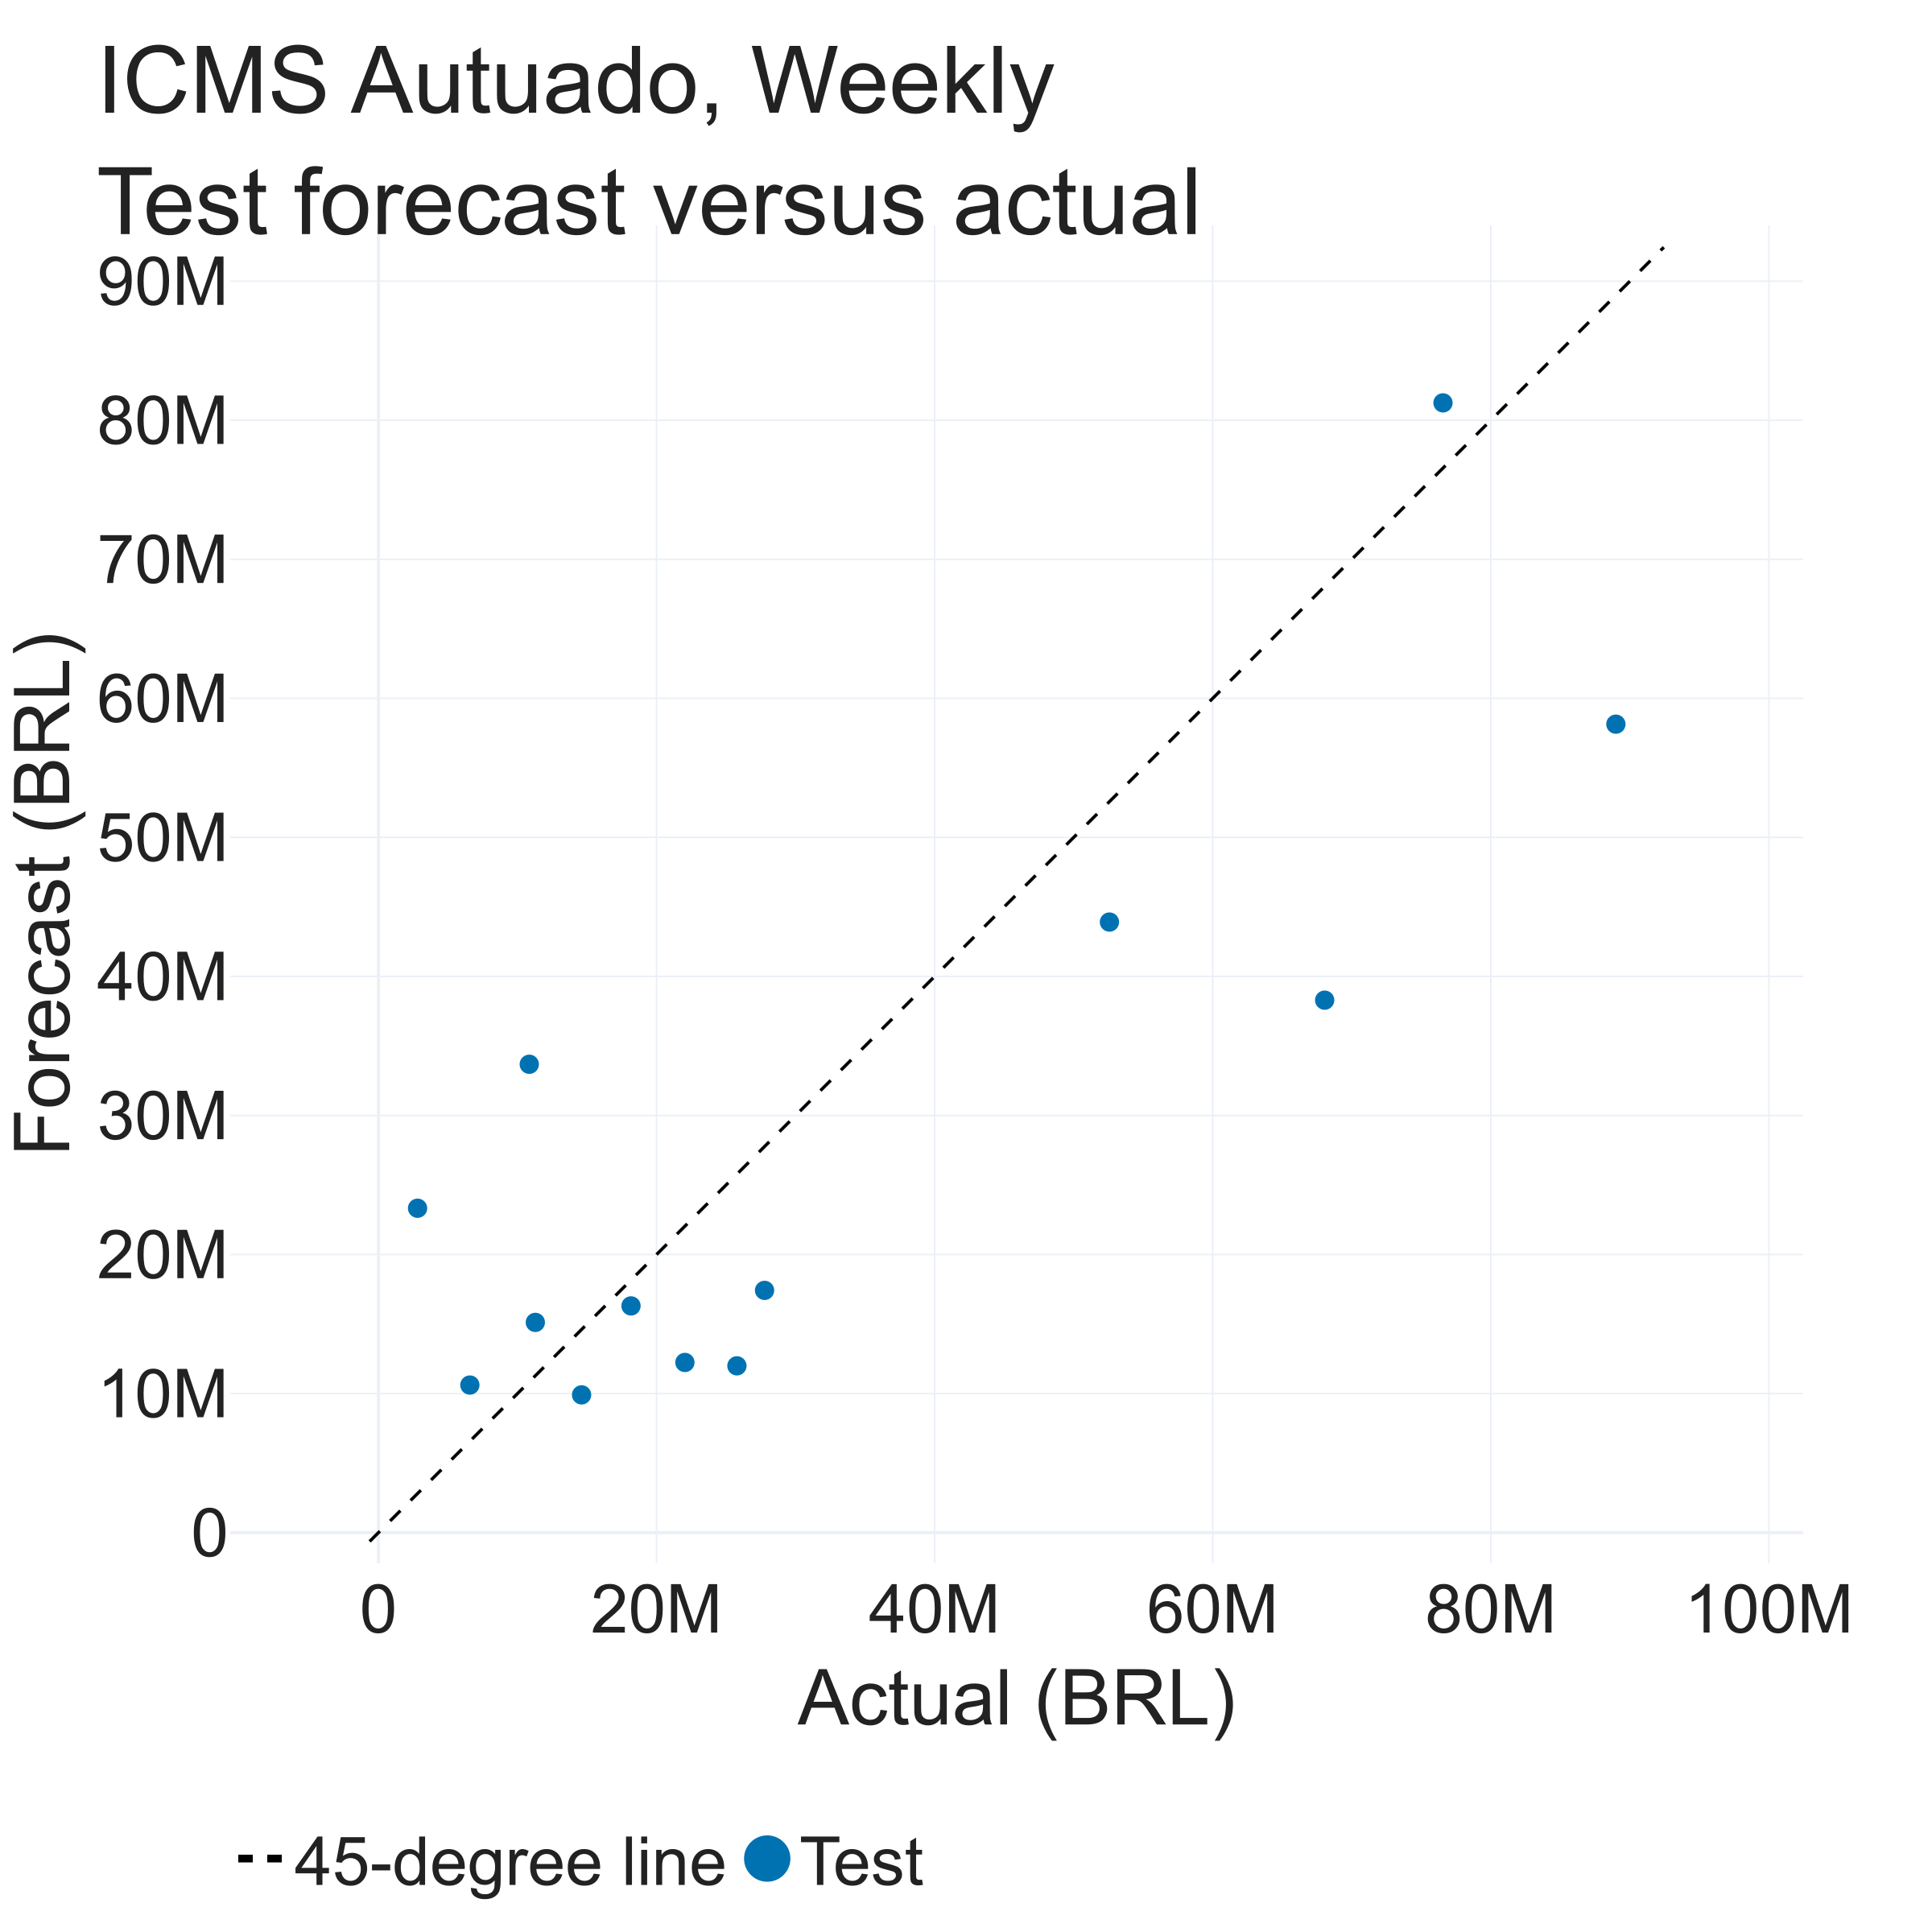
\includegraphics[width=0.62\linewidth]{figures/segment/autuado_weekly_scatter.png}
  \caption{Autuado, weekly test scatter.}
\end{figure}
\begin{figure}[H]
  \centering
  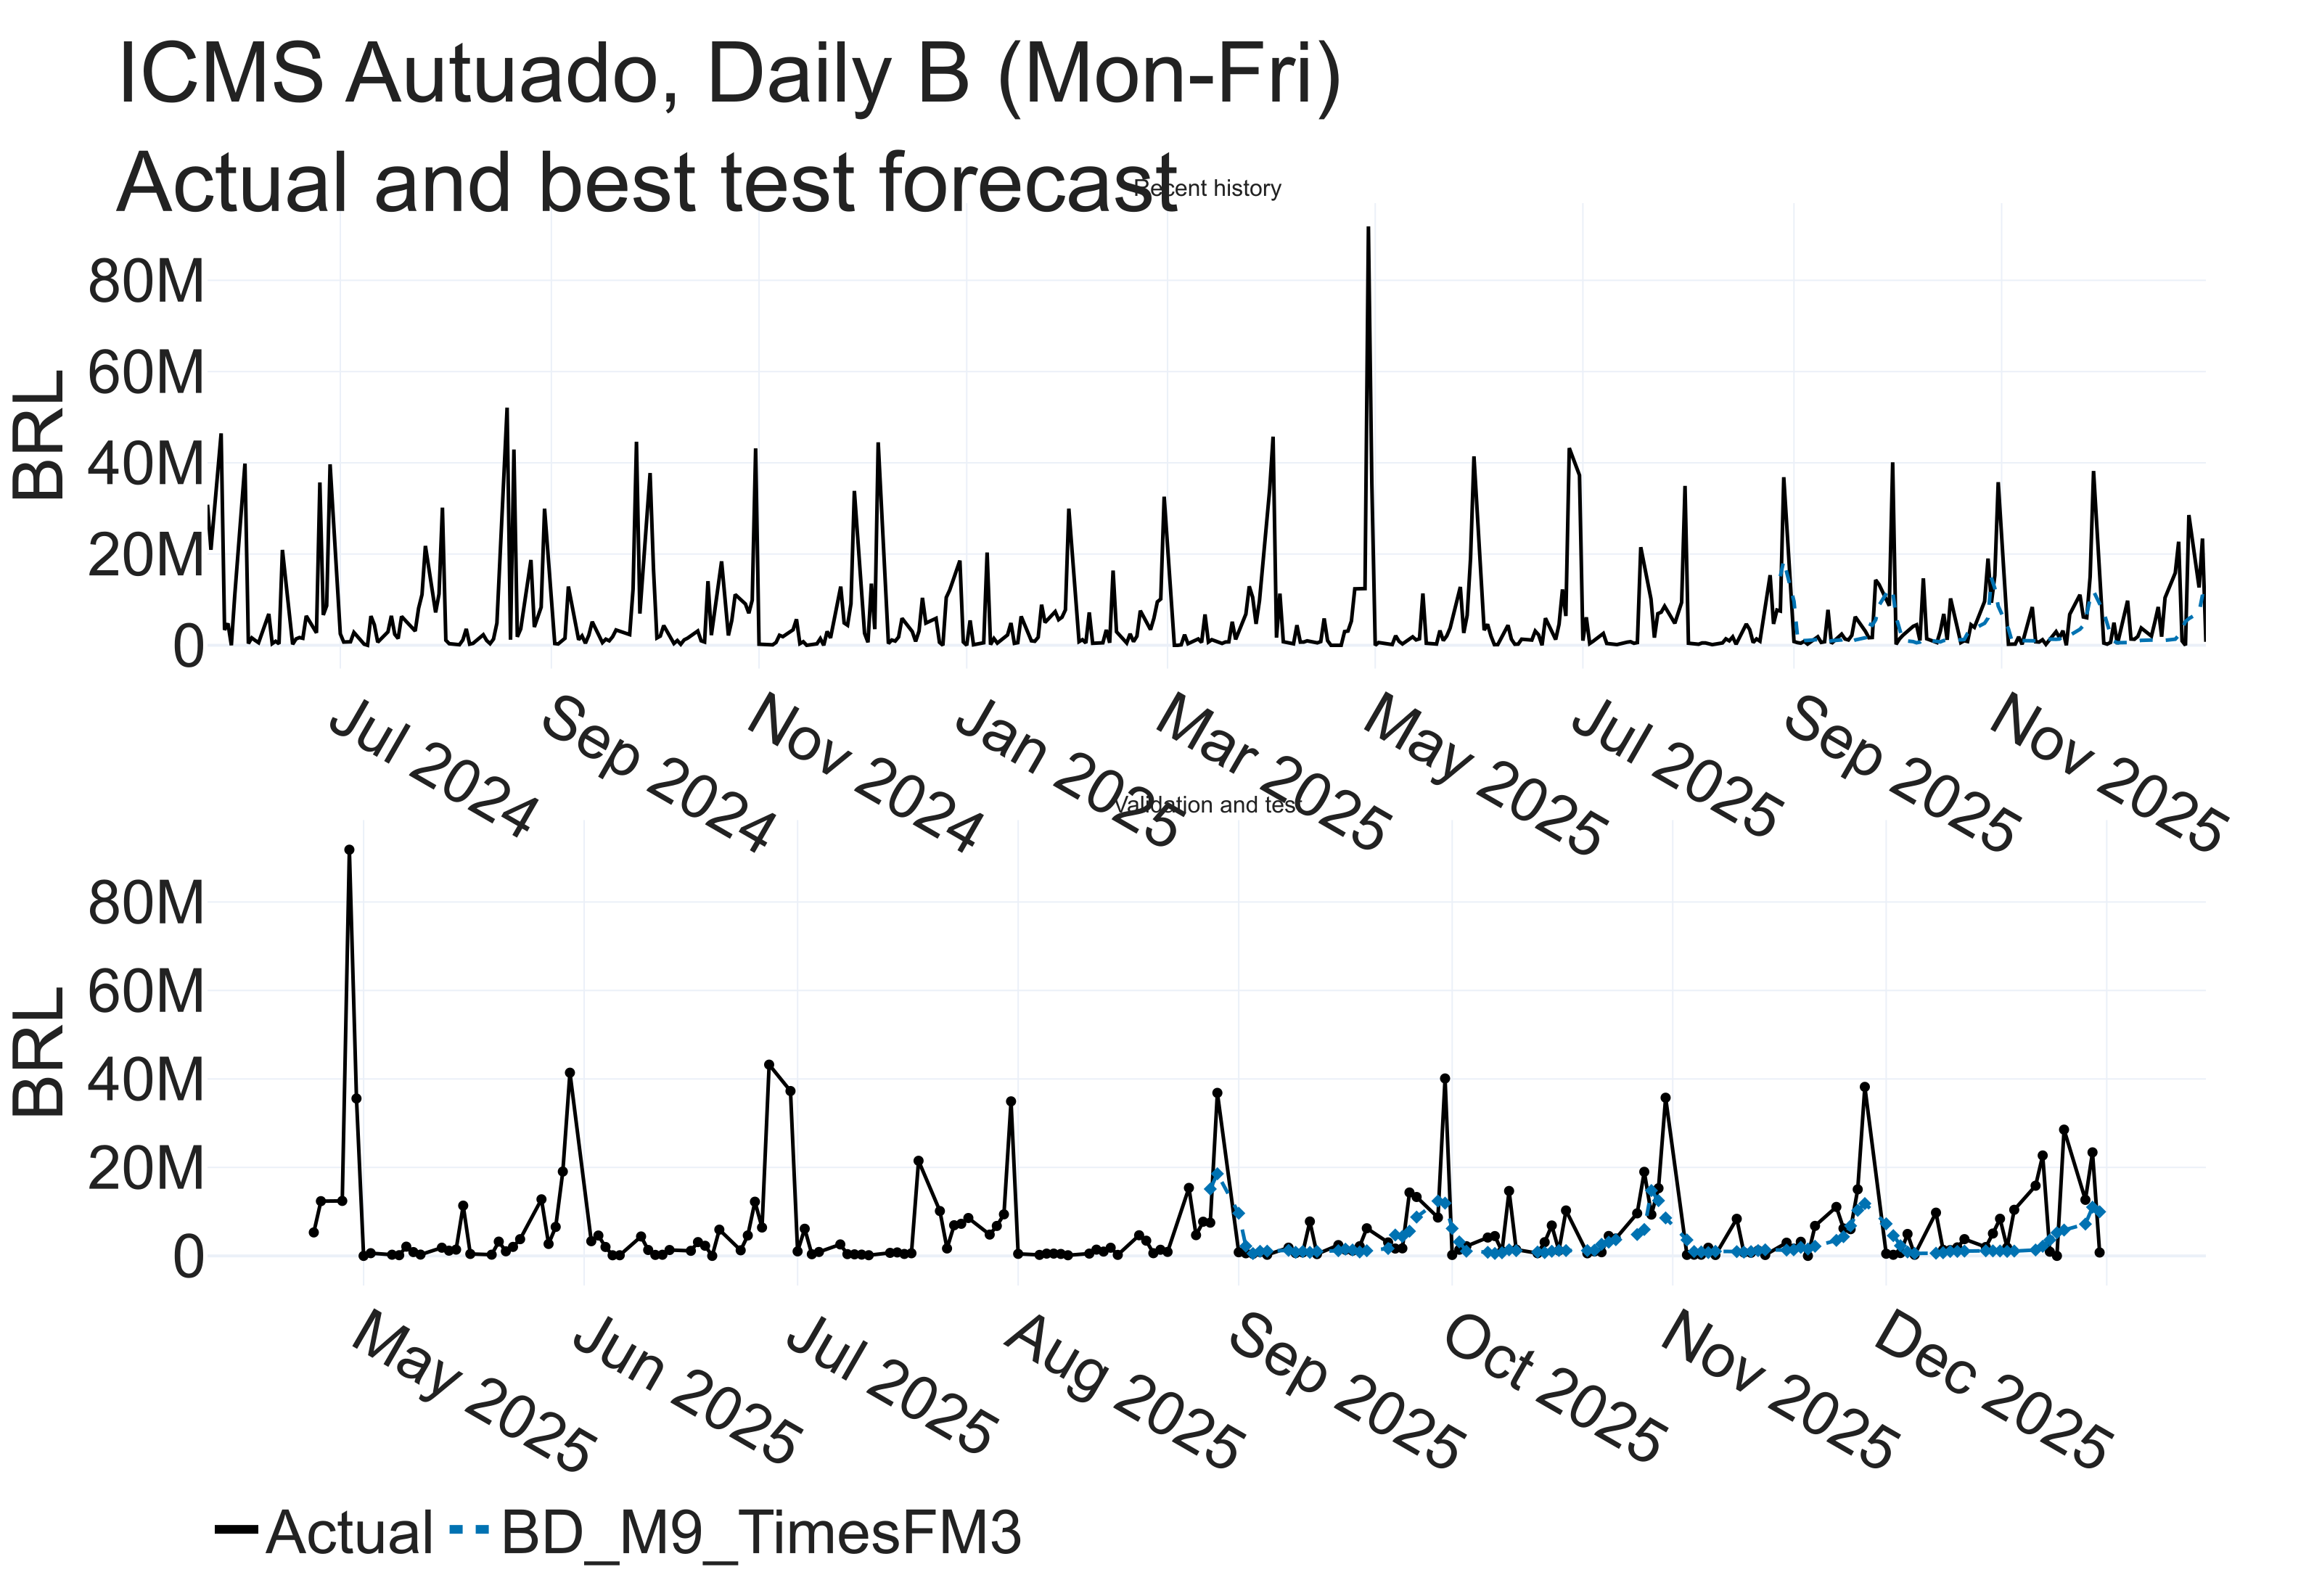
\includegraphics[width=\linewidth]{figures/segment/autuado_business_daily_forecast.png}
  \caption{Autuado, daily B. Blue dashed: M9 TimesFM.}
\end{figure}
\begin{figure}[H]
  \centering
  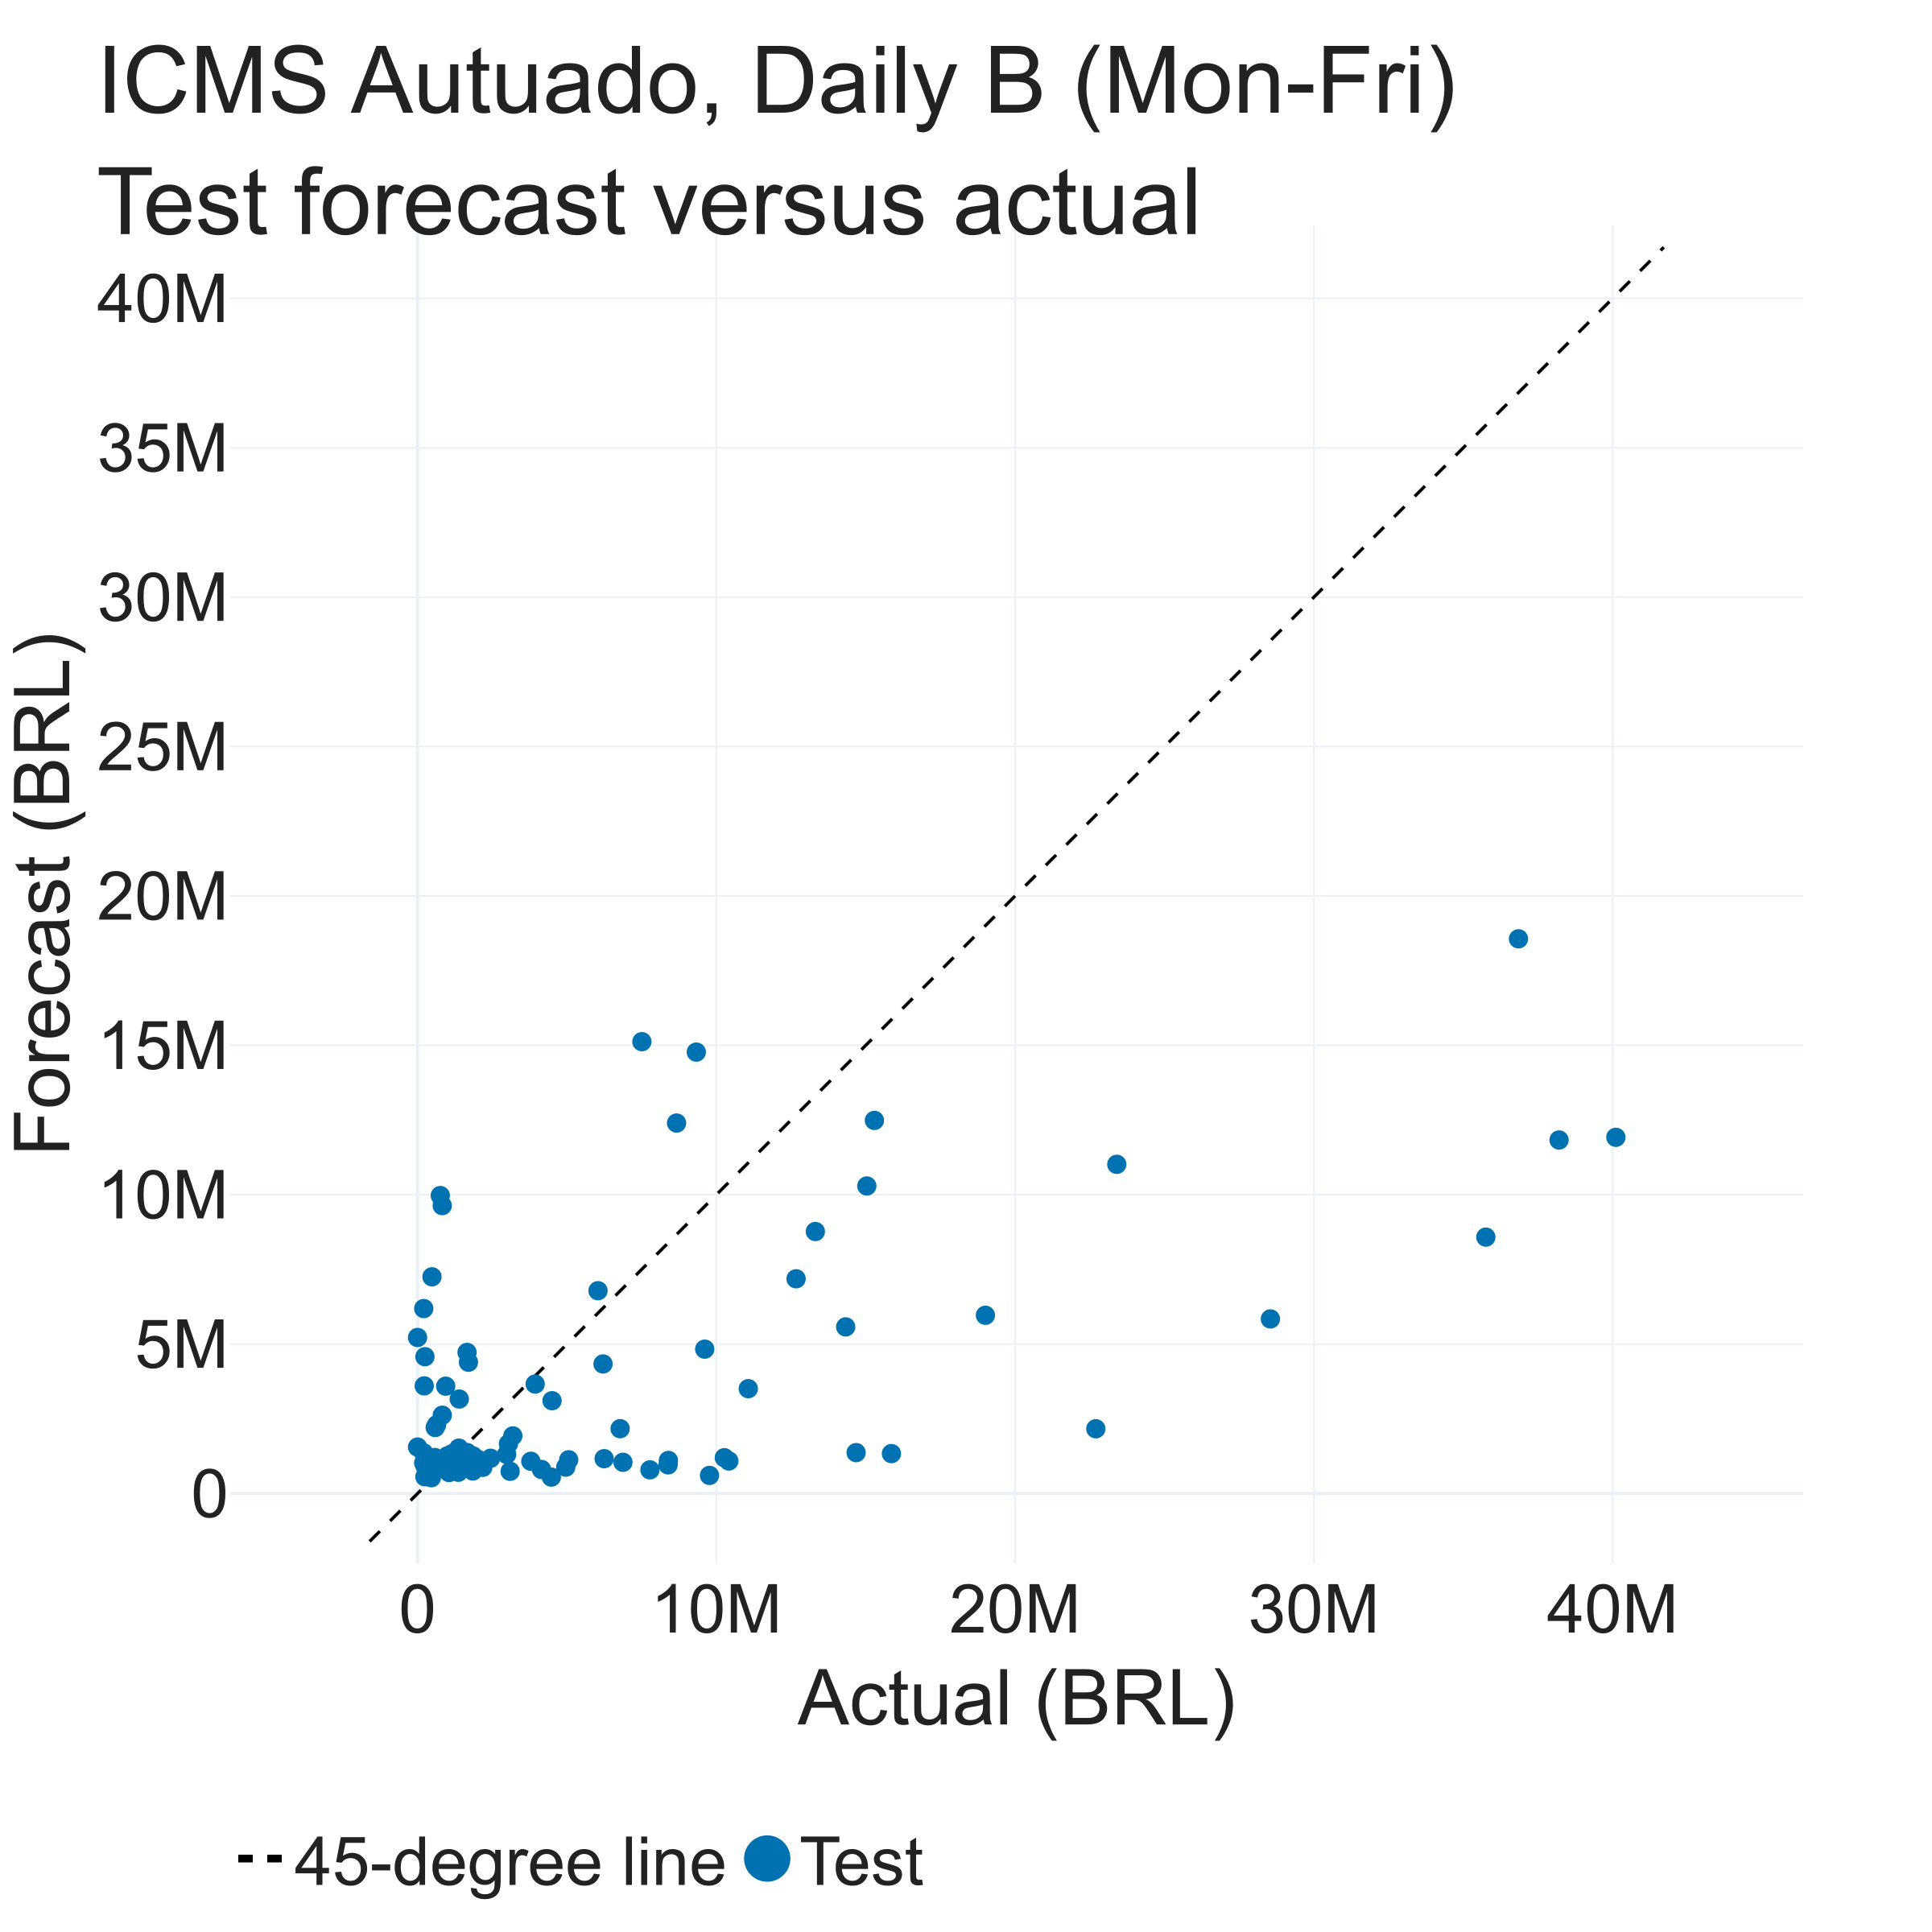
\includegraphics[width=0.62\linewidth]{figures/segment/autuado_business_daily_scatter.png}
  \caption{Autuado, daily B test scatter.}
\end{figure}
\begin{figure}[H]
  \centering
  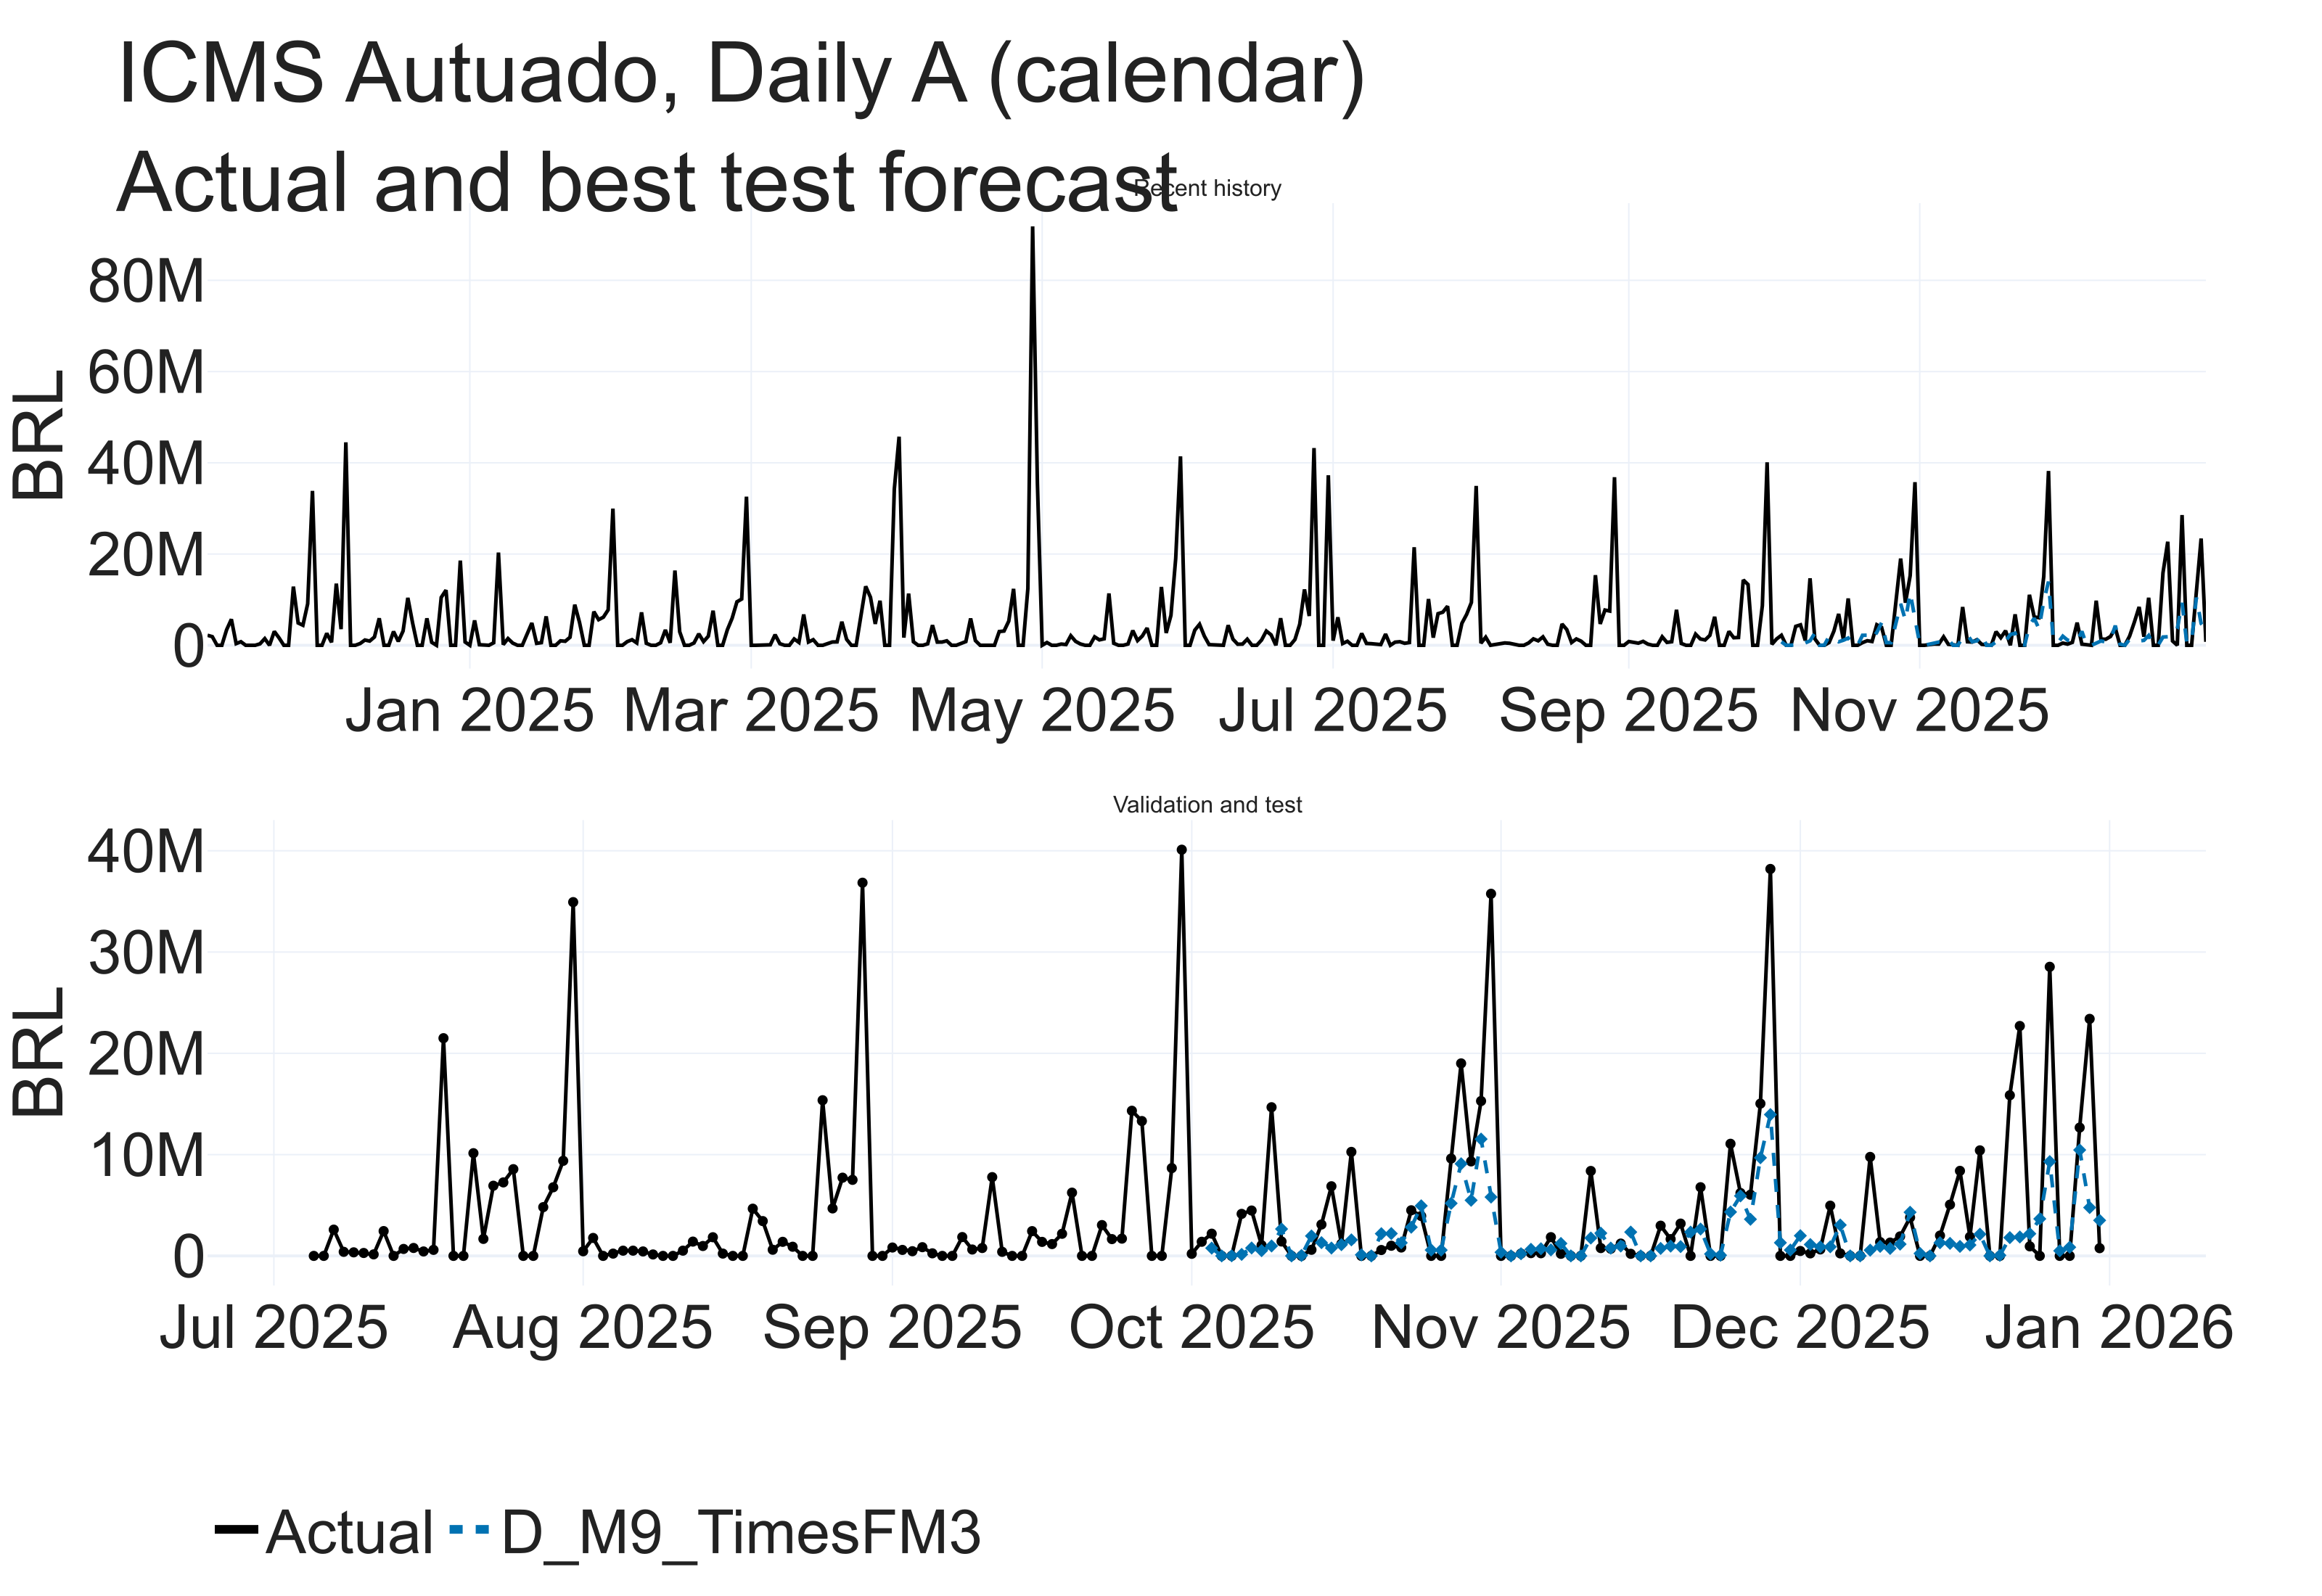
\includegraphics[width=\linewidth]{figures/segment/autuado_daily_forecast.png}
  \caption{Autuado, daily A. Blue dashed: M9 TimesFM.}
\end{figure}
\begin{figure}[H]
  \centering
  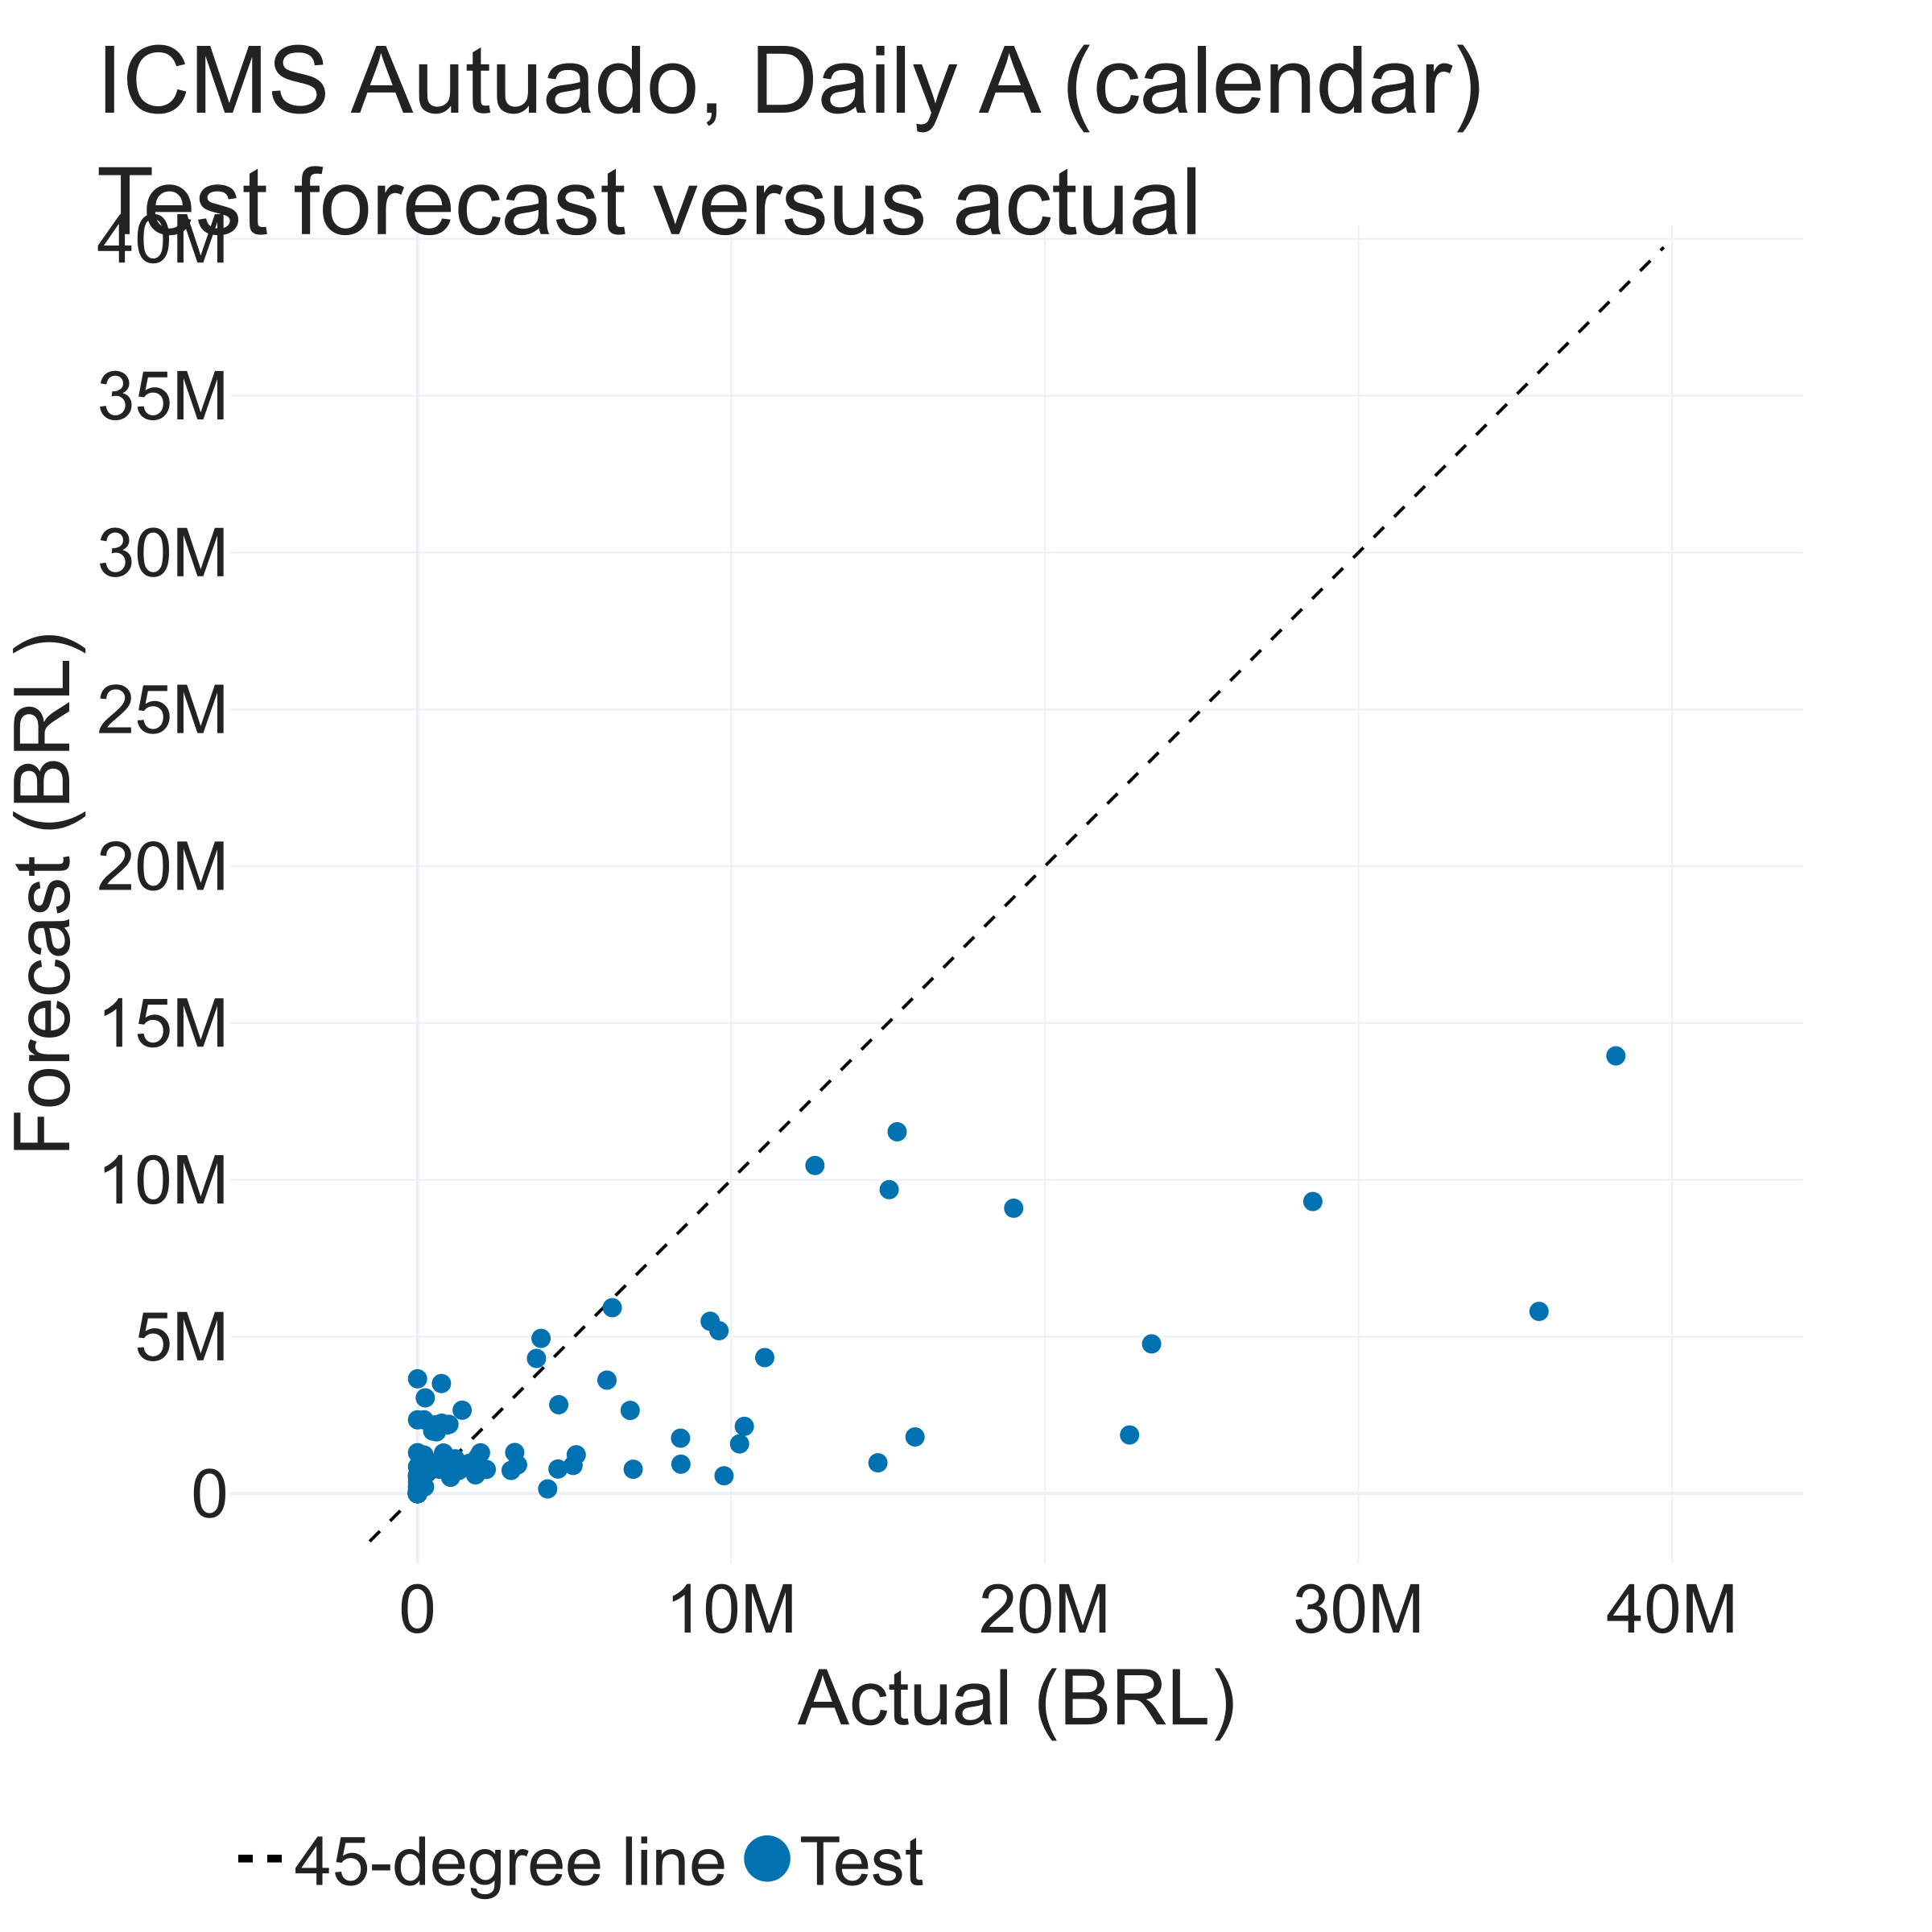
\includegraphics[width=0.62\linewidth]{figures/segment/autuado_daily_scatter.png}
  \caption{Autuado, daily A test scatter.}
\end{figure}


\bibliographystyle{plainnat}
\bibliography{refs}

\end{document}
